\documentclass{article}
\usepackage{enumerate}
\usepackage{amsmath}
\usepackage{amssymb}
\usepackage{graphicx}
\usepackage{subfigure}
\usepackage{geometry}
\usepackage{color}
\usepackage{bm}
\usepackage{indentfirst}
\usepackage{multirow}
\usepackage{hyperref}
\usepackage{listings}
\usepackage{xcolor}
\usepackage{url}
\usepackage{float}
\usepackage{array}



\graphicspath{{Images/}}
\lstset{
    columns=fixed,       
    numbers=left,                                        % 在左侧显示行号
    frame=none,                                          % 不显示背景边框
    backgroundcolor=\color[RGB]{245,245,244},            % 设定背景颜色
    keywordstyle=\color[RGB]{40,40,255},                 % 设定关键字颜色
    numberstyle=\footnotesize\color{darkgray},           % 设定行号格式
    commentstyle=\it\color[RGB]{0,96,96},                % 设置代码注释的格式
    stringstyle=\rmfamily\slshape\color[RGB]{128,0,0},   % 设置字符串格式
    showstringspaces=false,                              % 不显示字符串中的空格
    language=C,                                        % 设置语言
}


\begin{document}\large
\vspace*{0.2cm}

%\hrulefill

\thispagestyle{empty}


\begin{center}

\includegraphics[width=6cm]{logo}\\
\hrulefill
~\\
\begin{large}
\sc{\Large{UM--SJTU Joint Institute} \vspace{0.3em} \\ \Large{Design and Manufacturing I}  \vspace{0.6em}\\ \Large{VM250}}
\end{large}

\hrulefill

\vspace*{1cm}
\begin{Large}
\sc{{\Large{Project Report}}}
\end{Large}

~\\
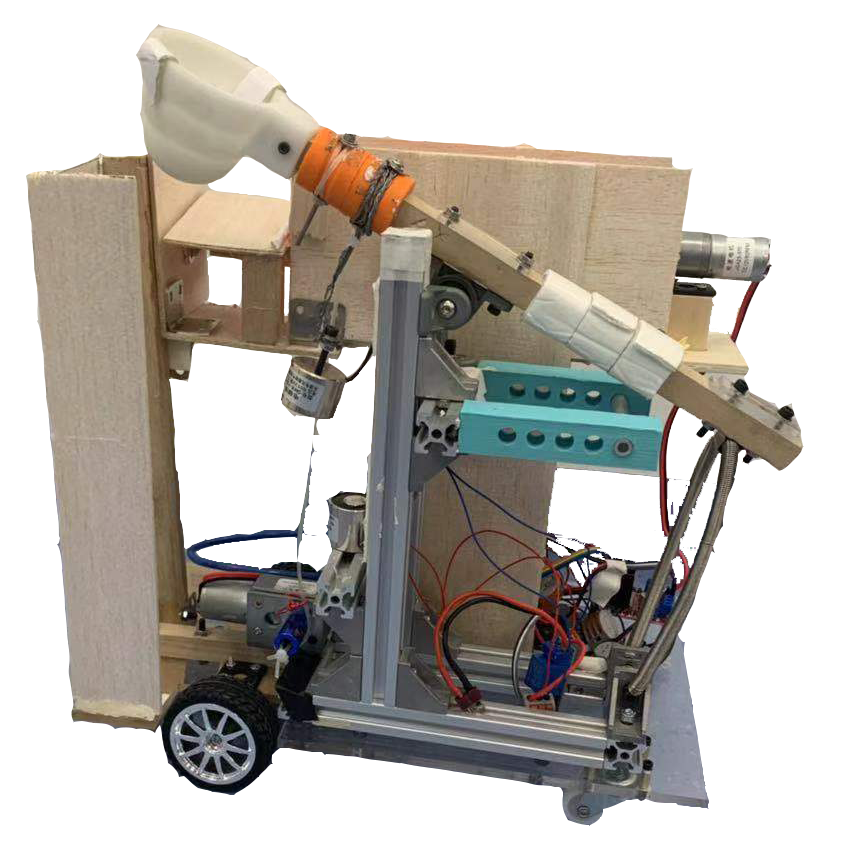
\includegraphics[width=7cm]{Car1}

%\vspace{2em}

\begin{large}
\sc{{
%%%%%%%%%%%%%%%%
%\Large{Lab 2}
%%%%%%%%%%%%%%%%%%
%\vspace{0.5em}
%%%%%%%%%%%%%%%%%%
%\Large{Measurement of Fluid Viscosity }%Title
%%%%%%%%%%%%%
}}
\end{large}
\end{center}


\vfill

\begin{table}[h!]
\flushleft
\begin{tabular}{lll}
Name: Wang Yuhao \hspace*{2em}&
ID: 517370910060\hspace*{2em}
& Group: 1\\
Name: Aleksei Danli \hspace*{2em}&
ID: 517370990024\hspace*{2em}
& Group: 1\\
Name: Jose Lasso \hspace*{2em}&
ID: 716370290067\hspace*{2em}
& Group: 1\\
Name: Chen Haoyang \hspace*{2em}&
ID: 517370910040\hspace*{2em}
& Group: 1\\~\\
Date: Aug 6th.
\hfill
\end{tabular}
\end{table}
\newpage
\tableofcontents


\newpage
%%-----CHY's part-----------
\section*{Abstract}
Our team is responsible for designing an automatic controlled metal trebuchet asked by TOYABC, a company for table toys. It should be made in a moderate size and controlled remotely. Our main goal is to shoot the balls accurately, operate smoothly and load different balls. Meanwhile, the design should not be too complicated so that the product will be easy to assemble and the materials of the product can be required easily. Also, the cost of production should not be too high. This final report will show you how our concepts are formed initially and being proved gradually. It will also include the advantages and disadvantages of our prototype.

\section{Introduction}
\subsection{Background}
The trebuchet is one of the ancient siege weapons, can put the stones into the walls of the enemy and the city, and cause damage.

\begin{figure}[H]
\centering
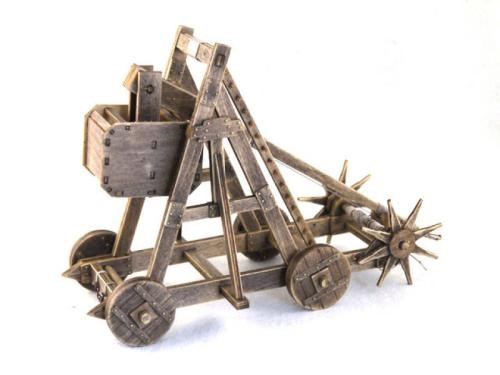
\includegraphics[width=0.6\linewidth]{treb}
\end{figure}
\subsection{Project Motivation}
As a part of design motivations, Inc., out team is asked by TOYABC, a company for table toys, to design an automatic controlled metal trebuchet or catapult, and then make a prototype using components provided with other necessary materials.
\subsection{Statement}
\begin{itemize}
\item Size: The prototype could be put into a $35cm*20cm*35cm$ box in any condition(with all components).
\item Movement: The prototype should be powered by at least one DC motor with batteries. There's no requirement on the speed of the prototype but the whole gaming time is limited.
\item Control: The basic movements of the prototype(moving in for directions, shooting ,reloading) should be controlled in a remote manner.
\end{itemize}
\section{Summary}
After discussing the problem’s requirements, we will then talk about out concept design. This part will include our problem definition, concept generation, concept selection, and embodiment design. Next we will show our manufacturing process. Followed is the cost and estimation for production cost. The last part will be the conclusion and the recommendation, meanwhile, the test results will also be provided in this part.
\section{Product Design}
\subsection{Problem Definition}
After doing research, we decide to make the design of our super launcher. We need to take several problems into consideration and make several drafts. To achieve the most effective method, we need to consider the difficulty of manufacturing and arrange our time better. We prepare at least one week for analysing and doing tests, so we should not spend too much time on manufacturing.
\subsubsection{Customer requirements(CR)}
What we need to consider first is customer requirements. These requirements are listed in the following.
\begin{itemize}
\item Size: The prototype could be put into a $35cm*20cm*35cm$ box in any condition(with all components).
\item Movement: The prototype should be powered by at least one DC motor with batteries. There's no requirement on the speed of the prototype but the whole gaming time is limited.
\item Control: The basic movements of the prototype(moving in for directions, shooting ,reloading) should be controlled in a remote way.
\end{itemize}

After taking these three requirements into consideration, we can reach the customer requirement showing below.

\begin{figure}[H]
\centering
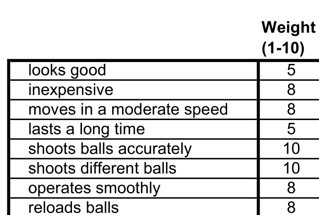
\includegraphics[width=0.5\linewidth]{cr}
\caption{Customer Requirements(CR)}
\end{figure}

We list "shoots balls accurately" and "shoots different balls" as the most important requirements. Shooting balls accurately is without doubt the most elementary requirements since the trebuchet is used for shooting. Also, shooting different balls is very important since we need to shoot three different balls in total. So, we need to pay attention the adjusting the strength of casting. Other requirements such as operating smoothly and moving in a moderate speed should also be put emphasis on since they are helpful in improving the efficiency of the whole operation.
\subsubsection{Engineer Specification(ES)}
The related engineer specification is listed in the QFD chart in the next part. The specifications will be discussed further later.
\subsubsection{Qualify Function Development(QFD)}
\begin{figure}[H]
\centering
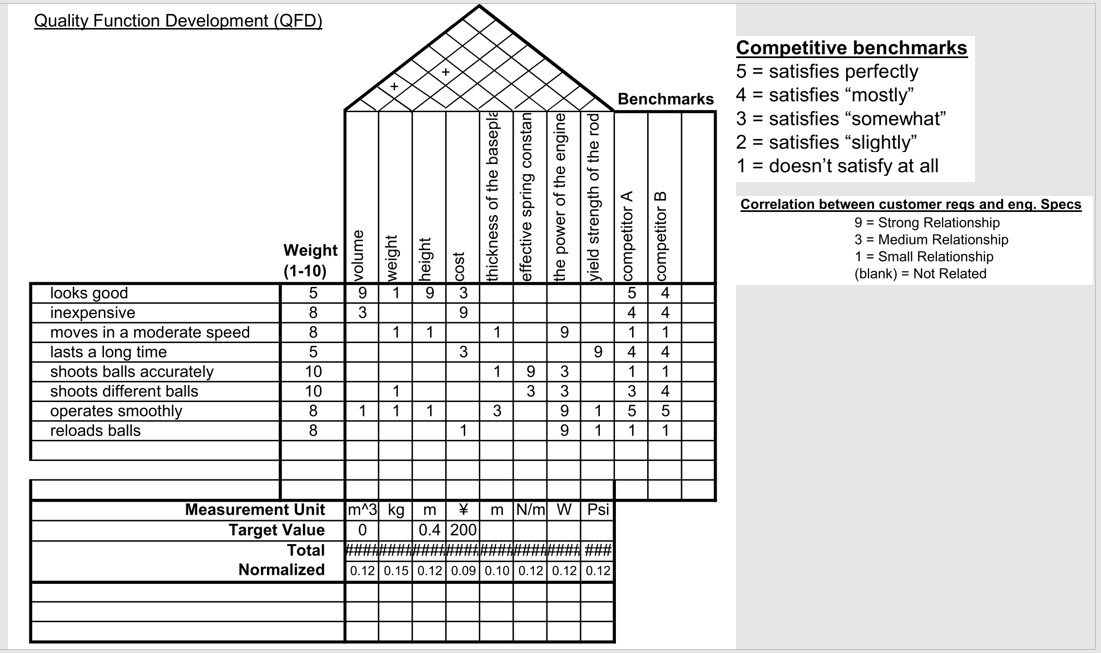
\includegraphics[width=1\linewidth]{qfd}
\caption{QFD}
\end{figure}
\subsubsection{Product Design Specifications (PDS)}
\begin{enumerate}
\item Performance: The speed should be moderate in order to keep the launcher more stable. Also, it will be easier to control the speed.
\item Size: the prototype should be fit into a box $35cm*20cm*35cm$.
\item Weight: The weight of the prototype should be moderate in order to keep the launcher more stable.
\item Materials: We need to choose affordable but practical materials. They should be easy to purchase or manufacture. The intensity of the rods should be strong in order to afford the compact of shooting.
\end{enumerate}

%
%-----------------------------------
%
\subsection{Concept Selection}
\subsubsection{Go/no-go Screening}
After discussion, we chose trebuchet as our design because utilizing the given extension springs in this way is more convenient for achieving the goals, compared to using catapult. \\

\begin{figure}[h!]
\centering
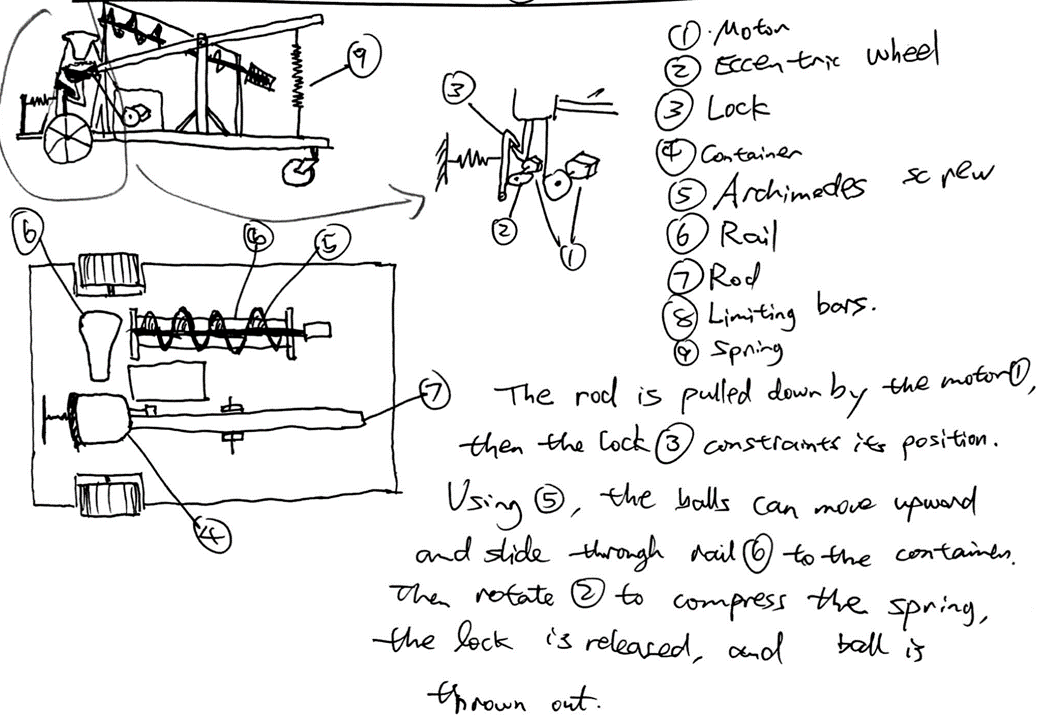
\includegraphics[width=0.8\linewidth]{Concept}
\caption{The concept diagram for the car.}
\end{figure}
~\\

As shown in this figure, the car is composed of four sections: controlling, moving, reloading and shooting. Now let's focus on some of the following specifications in this section.
\subsubsection*{Shooting Component}
The shooting component is very crucial for this project. Good reliability and accuracy of this part greatly influences the final success. It is typically composed of these components: the container for different sizes of balls, the beam, the gear motor, the electromagnetic (working as the fixing \& releasing part) and the frame for the shooting structure.\\

$\blacktriangleright$ Container
\par In our designing process, we planned to use a disposable meal box (round shaped) to achieve the goal for holding the ball and throwing this out. And fillers such as foam can be applied to the inner part to act as a buffer layer. However, through our testing, we found out that using this meal box is quite large in terms of its size, and large \& heavy so that it's becoming a tough problem for us to throw the balls. Therefore, we plan to manufacture the "bowl" using 3D printing technology.\\

In our designing part, we planned to make a bowl that could support all the three balls in a tight manner. Therefore, we drew the inner part of this bowl according to the measured diameter of the three bowls. (see figure below)\\
\begin{figure}[H]
\centering
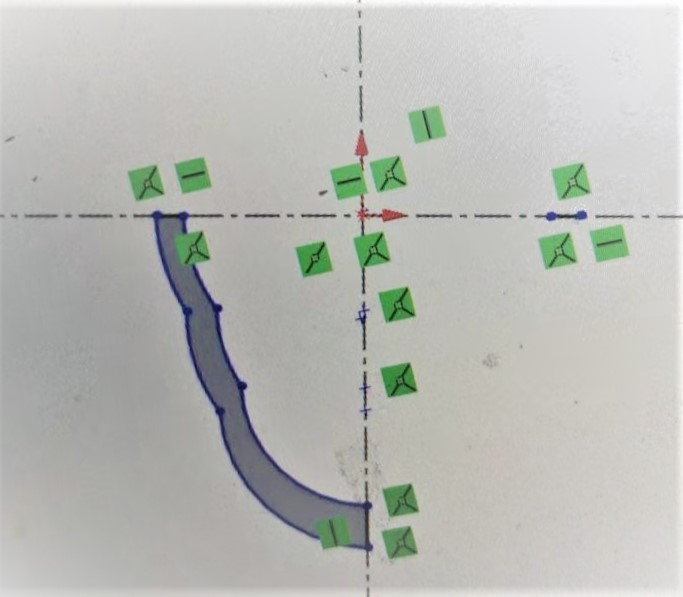
\includegraphics[width=0.3\linewidth]{Bowlsketch}
\caption{The sketch of the inner part of the bowl.}
\end{figure}
~\\

Then we extruded this sketch, and added a connecting part to the beam, got the following final version of the designed bowl:\\

\begin{figure}[H] 
\centering 
\subfigure{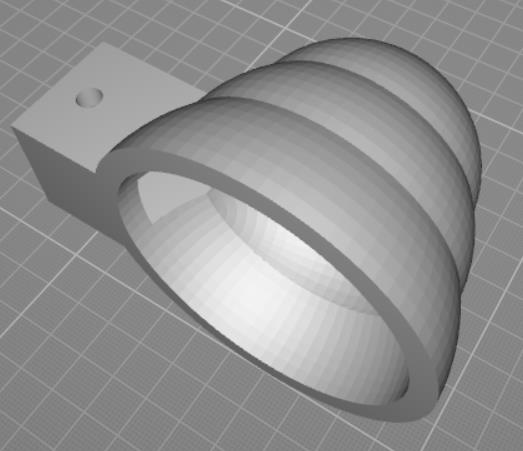
\includegraphics[width=0.37\linewidth]{Bowl1}
}
\subfigure{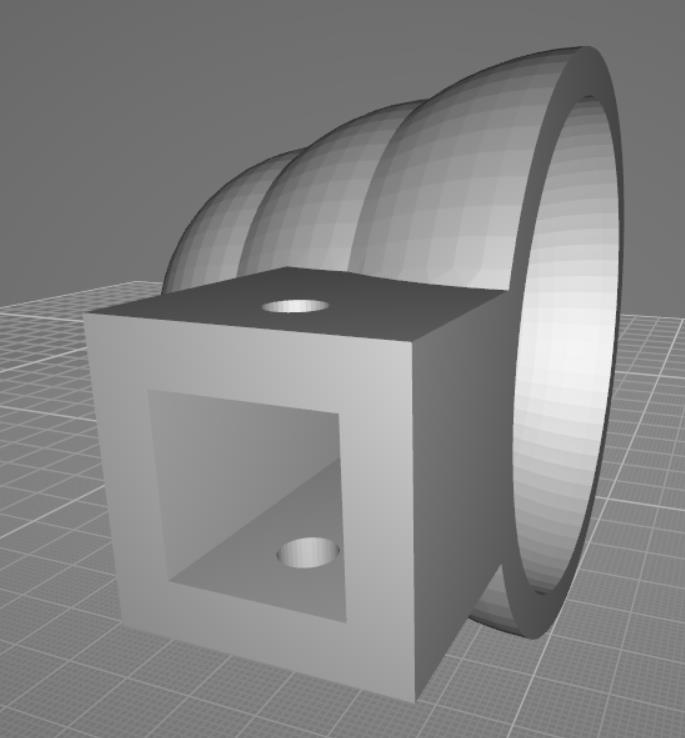
\includegraphics[width=0.3\linewidth]{Bowl2}
}
%\label{fig-sample-1}
\caption{The CAD design for the bowl.}
\end{figure}

When the bowl was printed out, we found that the friction inside the bowl was so large that this could not throw the ball out so smoothly as we think, thus we added a piece of foam tape to reduce the friction inside.

\begin{figure}[H]
\centering
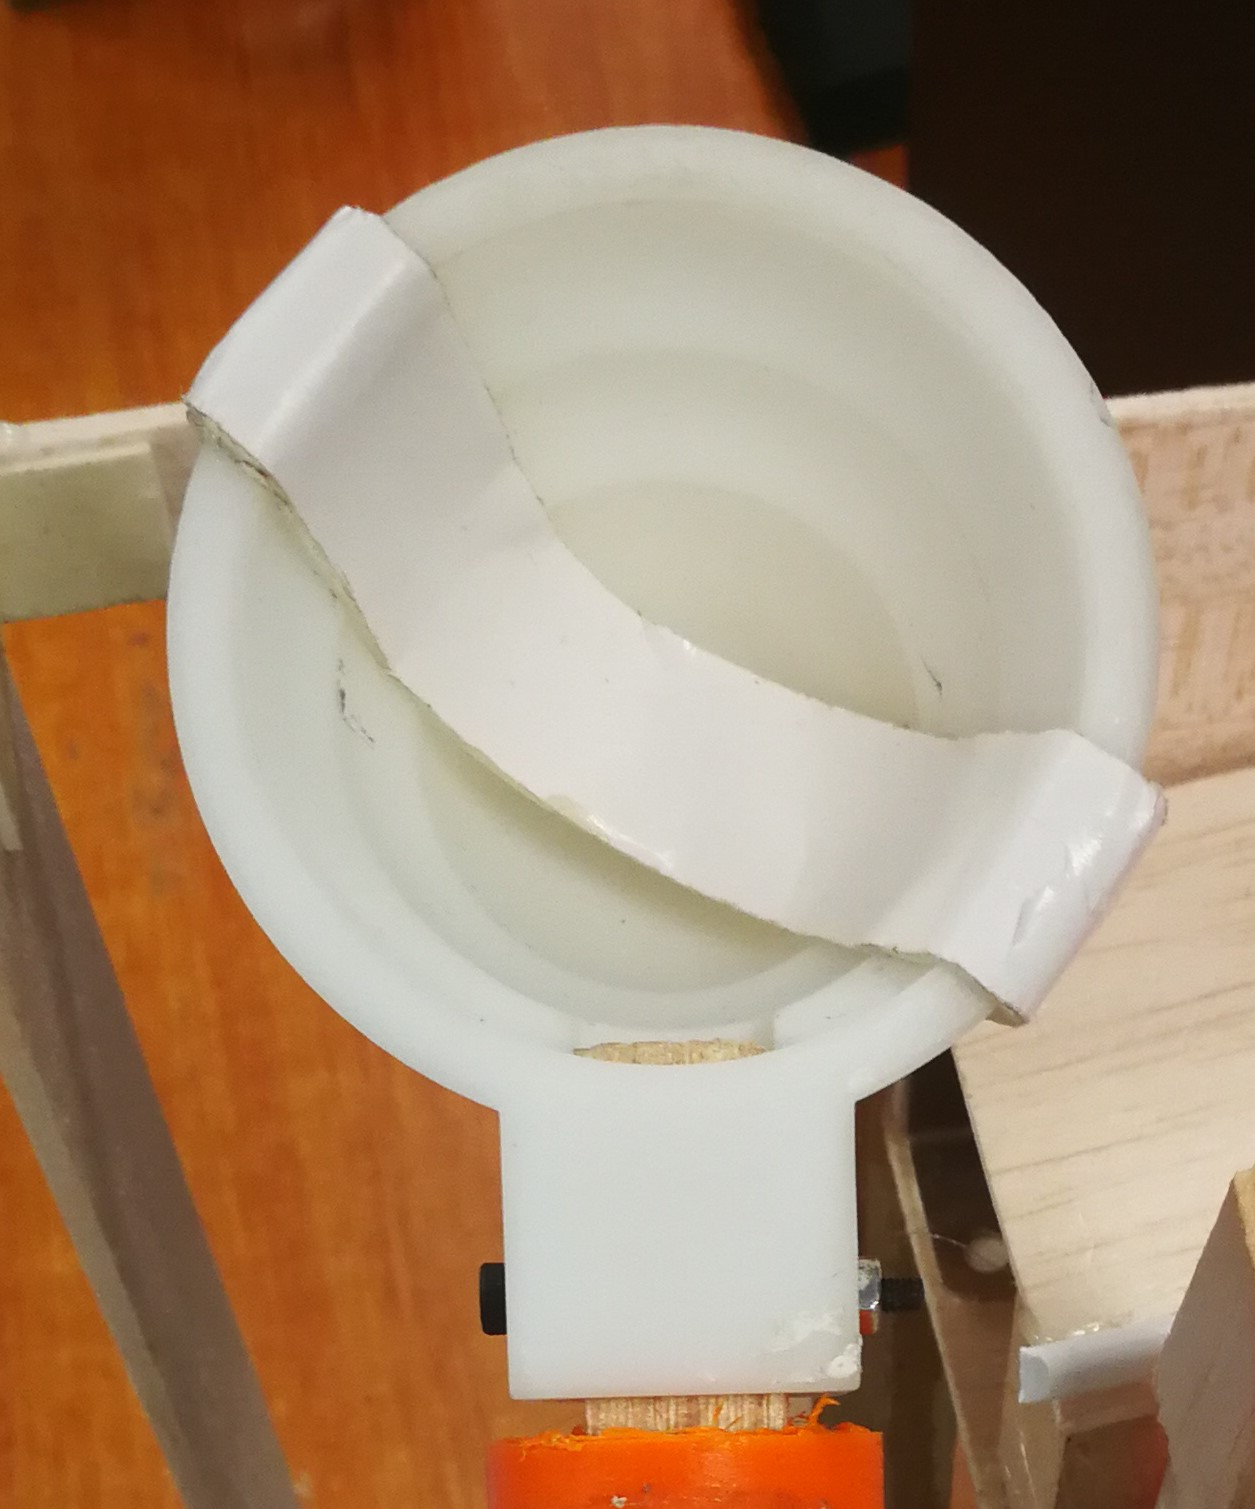
\includegraphics[width=0.3\linewidth]{Bowl3}
\caption{The real version of modified bowl.}
\end{figure}
~\\

$\blacktriangleright$ Beam
\par For our project, we chose wood as the beam for the throwing part. The weight of the wood is light, and it is easy for us to do operations onto the wooden beam such as hole drilling. We chose the cross-sectional area of the beam as $15mm\times 15mm$ so that it fits well to our designed bowl.


\begin{figure}[H]
\centering
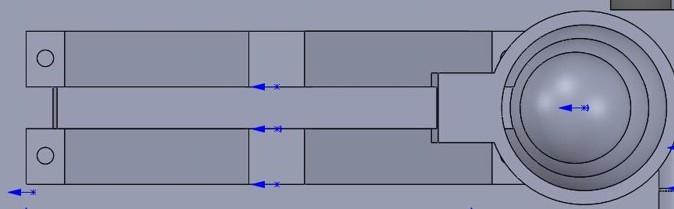
\includegraphics[width=0.6\linewidth]{arm}
\caption{The CAD beam design.}
\end{figure}
~\\


$\blacktriangleright$ Gear motor\\
\par The gear motor is a key component for our design of the pulling of the beam. As it needs to drag the whole beam with the ball down, competing with the spring force, then it requires much force to proceed this. Through our testing using the \textbf{pressure gage}, the estimated force is around $5.2 kg$.\\

To achieve this, the common practice is to use a gear motor, a stepper motor, or a servo motor. Through our consideration, we found the following disadvantages of the latter two kinds:
\begin{enumerate}
\item The servo motor is not so stable during the usual operation compared with using the normal motors. Parts inside may easily get burnt once the external force blocks its shaft.
\item The coding for the servo motor is more complicated than that of the normal one.
\item The stepper motor is very heavy, approximately 5 to 6 times of the weight of a normal gear motor. Also, its driver board is too space-consuming, which is not ideal for our intense-volume designed prototype.
\item Using the stepper motor require more ports that connect to the control unit (Arduino board), and managing these wires creates more tasks for us.
\end{enumerate}
\par Using the torque data given by the dealer for the gear motor, we chose the 12V 36 RPM DC motor as the pulling part, which is quite ideal in terms of both the rotation speed and required force.

\begin{figure}[H]
\centering
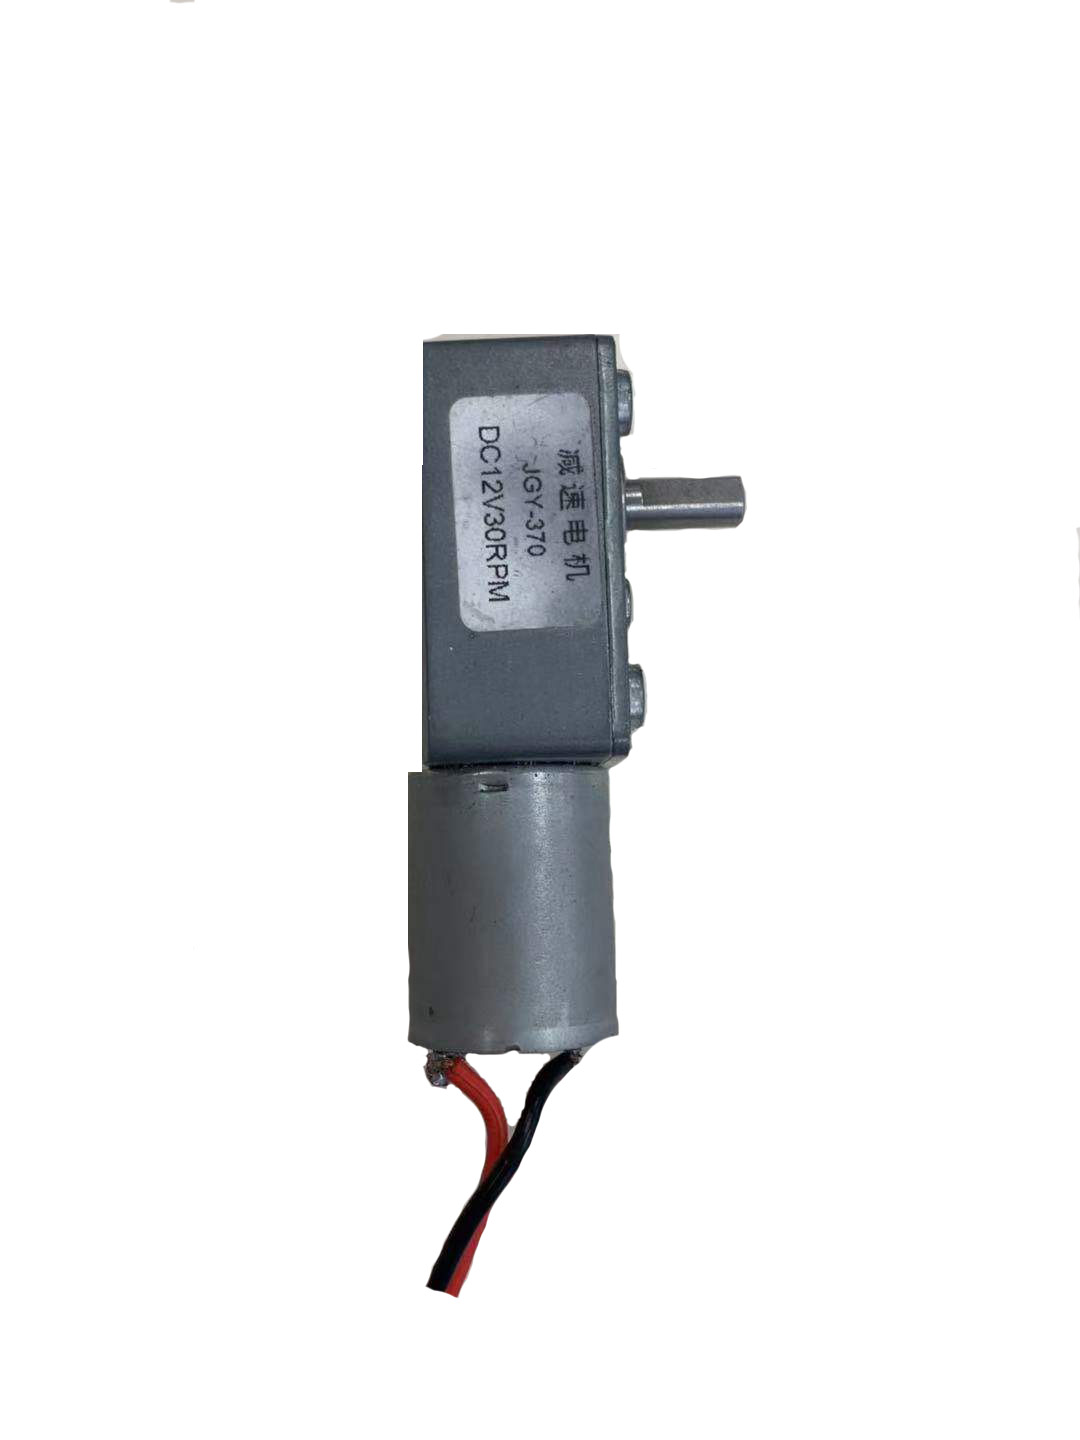
\includegraphics[width=0.35\linewidth]{1}
\caption{The gear motor chosen.}
\end{figure}

\par To connect the string to the beam from the motor, we created a circular stand with gap in its outer rim, and a $15mm\times 15mm$ square was extracted from its top to the bottom so as to cover the wooden beam. Also, holes are designed in line with the drilled hole on the beam so that this component can be fixed tightly to the beam while the deformation to the beam can be minimized as the force that the string exerts onto the beam can be distributed evenly, rather than being concentrated into one point.


\begin{figure}[H]
\centering
\subfigure{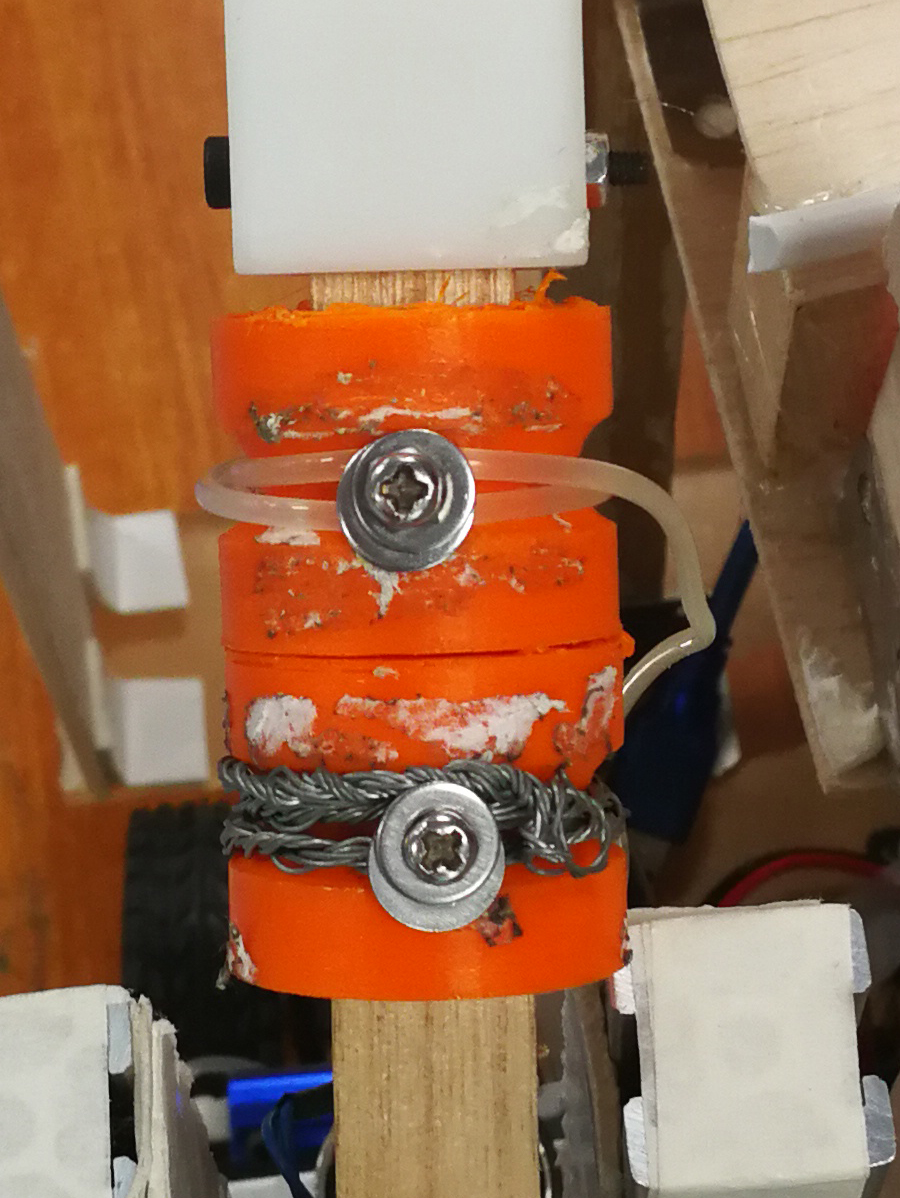
\includegraphics[width=0.2\linewidth]{Stand}}
\subfigure{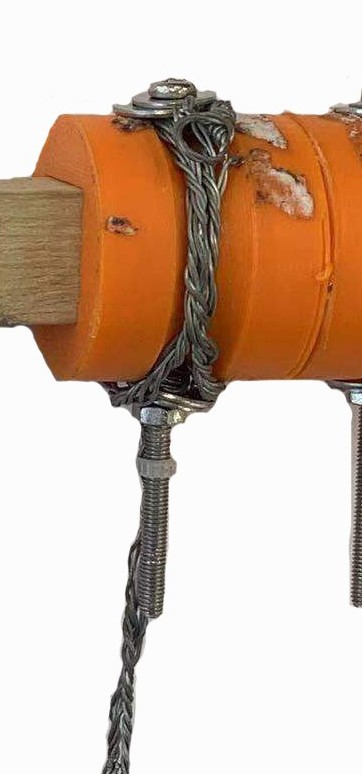
\includegraphics[width=0.14\linewidth]{711}}
\caption{The real image of the circular stand.}
\end{figure}
~\\

$\blacktriangleright$ Electric magnet\\
The first version of design for the releasing part is to make a self-lock structure when the beam is pulled down, and a rotating cam for releasing the lock. The diagram is shown below.
\begin{figure}[H]
\centering
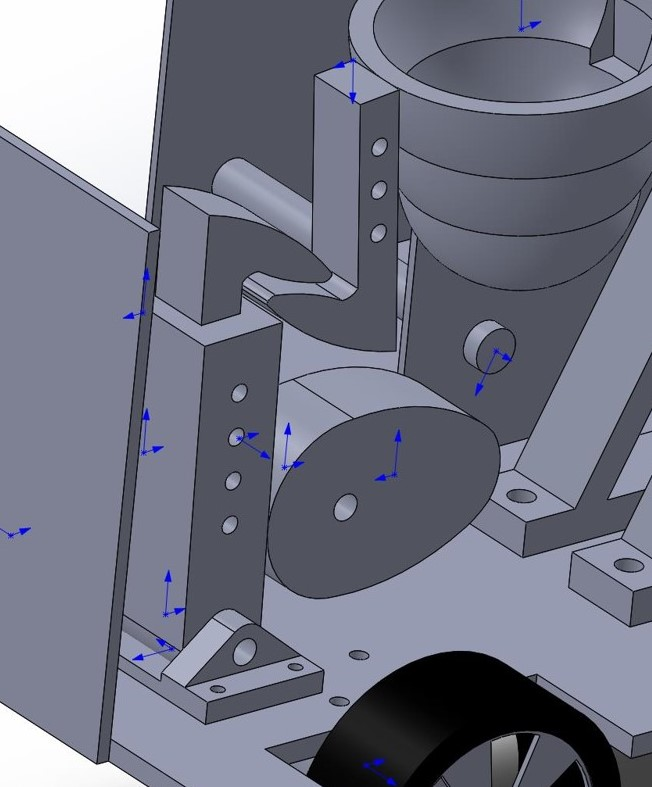
\includegraphics[width=0.4\linewidth]{Lock}
\caption{The original lock structure.}
\end{figure}
~\\
However, considering the complicity of this structure, which is both hard to build and unstable due to the large force this part needs to endure, we had to find an alternative solution. And when we paid our attention to the electromagnet, we could clearly see its benefits:
\begin{enumerate}
\item We just need one extra electric relay to control its operation -- easy for coding and arrangement.
\item Easy to fix this to the frame of the structure.
\item Doesn't consume the power too much. Can be supplied by a 2200mAh Li-ion battery throughout the whole 10-min game.
\end{enumerate}
\par Therefore, we chose the electromagnet as the fixing \& releasing part. We attach one magnet onto the frame of the shooting structure, fixed onto an aluminum beam whose height can be easily adjusted, and the other tied to the beam using the same circular stand. In this way, when the string pulls the beam down and we connect the magnetic to the power supply, it fix the position of the beam. When we cut off the power supply, the bar will be released and balls will be shot.\\
\begin{figure}[H]
\centering
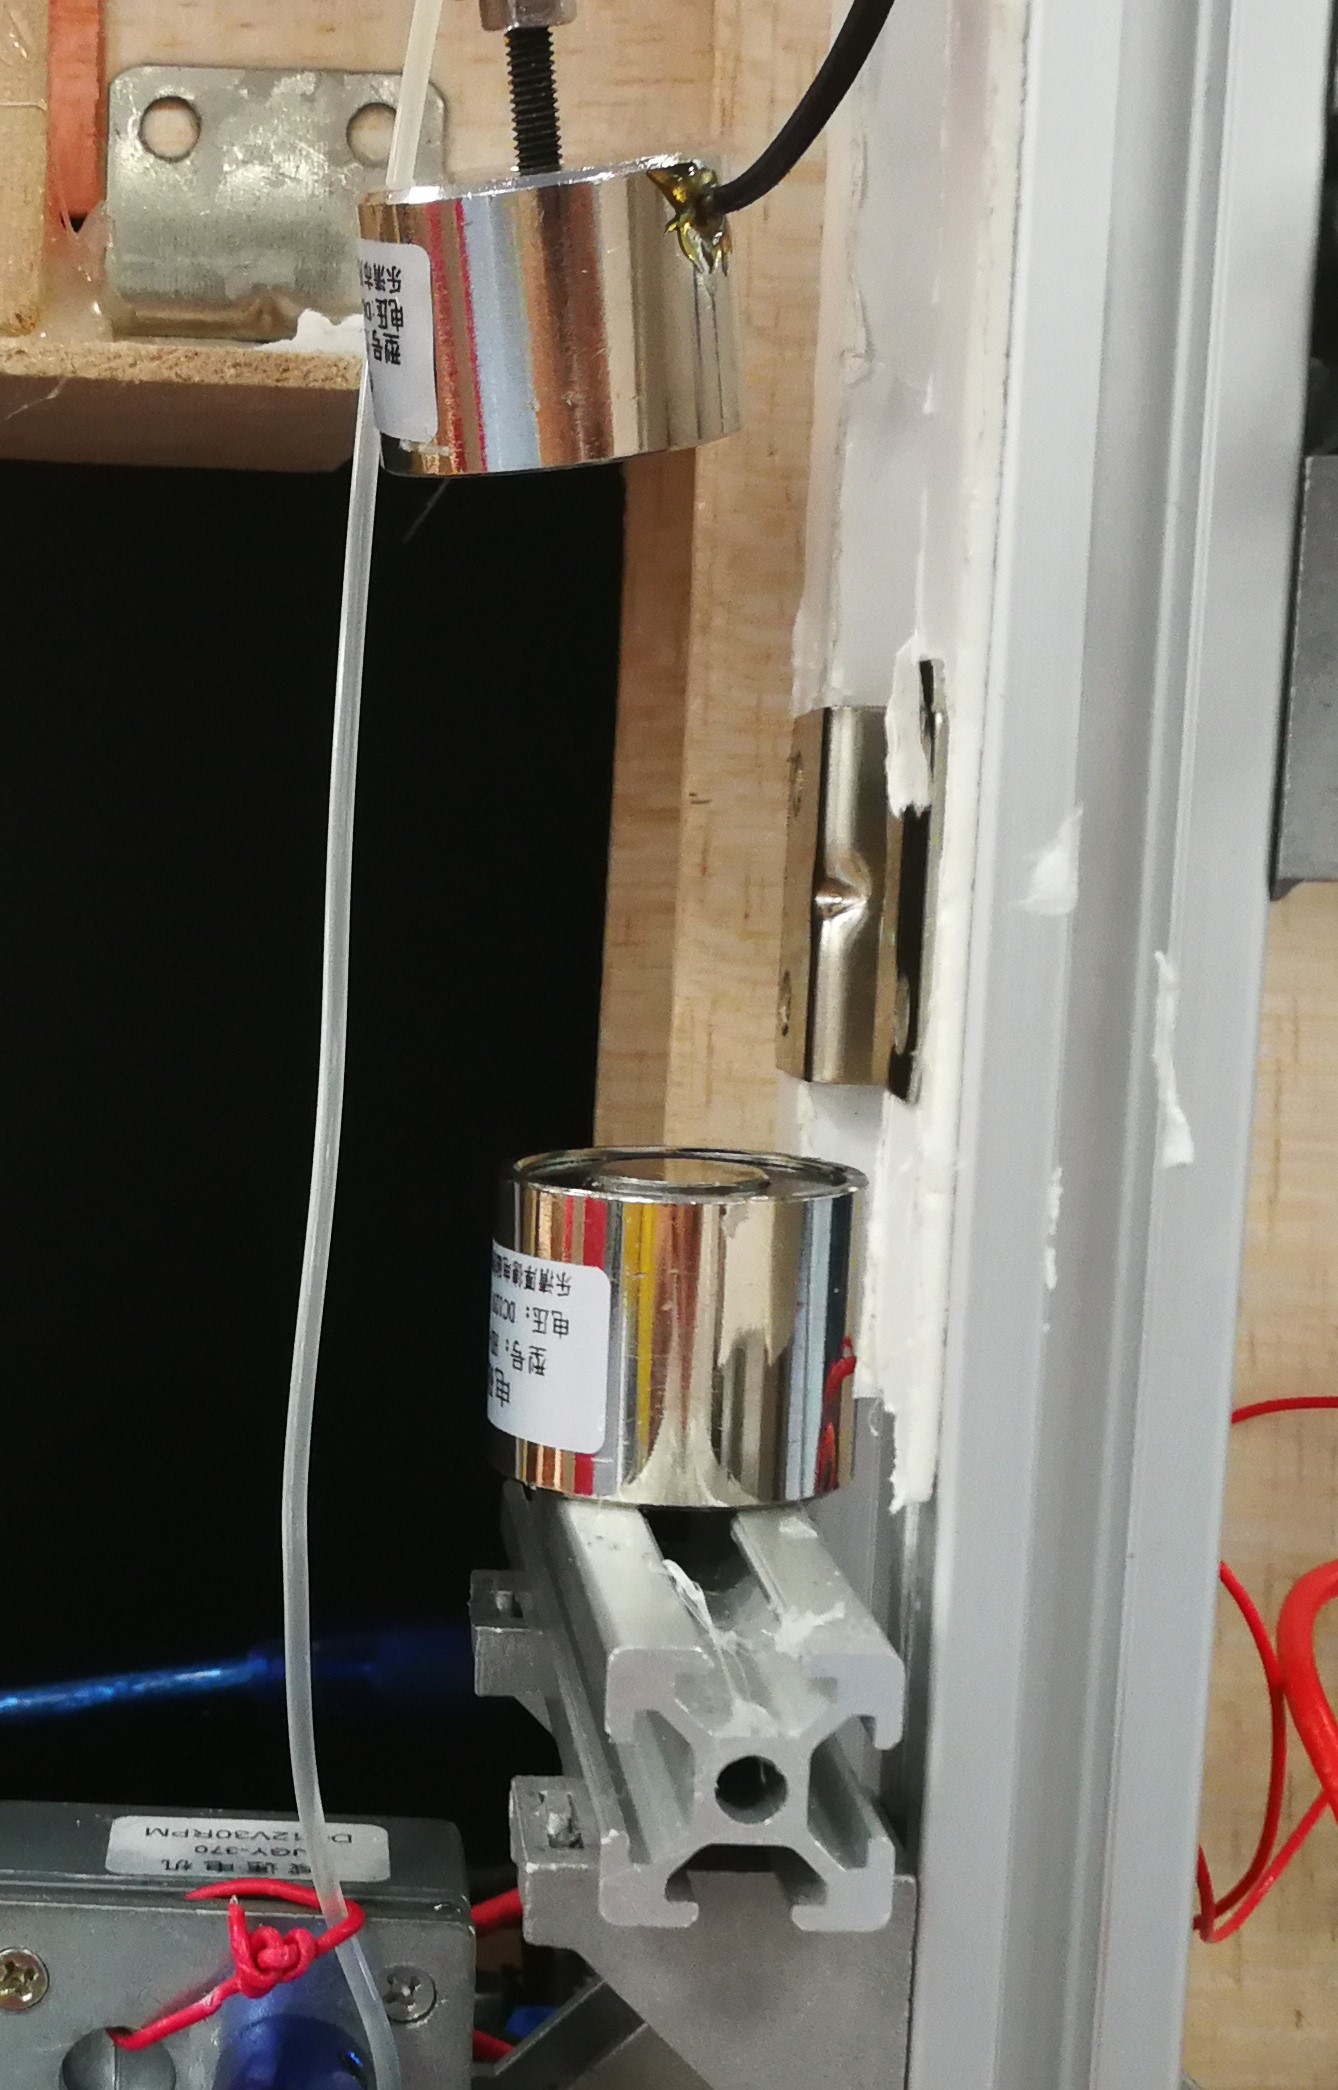
\includegraphics[width=0.3\linewidth]{Elec}
\caption{The electromagnet.}
\end{figure}


$\blacktriangleright$ The frame of the whole structure
\par In our previous design, we planned to use a 3D printed stand to fix the rotation beam. After later consideration, we found that there are several problems related to this:
\begin{enumerate}
\item Most of our 3D printed parts use PLE material and printer, and these materials cannot tolerate very large force.
\item During later testing procedure, we may need to change the position of the beam for the sake of accuracy. Using the 3D printed components may not provide enough flexibility for this.
\item The bottom of this structure need to be stable and absorb shock as much as possible. It's quite hard to reach the balance between this stability and low space occupation.
\end{enumerate}
\par Then we pay attention to the 2020 alumium extrusion. 2020 means the cross sectional area of this extrusion is $20mm\times 20mm$, with the detailed sketch shown below. Such kind of extrusion provides us the flexibility to build the desired frame through the combination with appropriate kinds of angled irons. Meanwhile, the strength, stability and its property of low mass enables this structure to satisfy our needs. 
\begin{figure}[H]
\centering
\subfigure{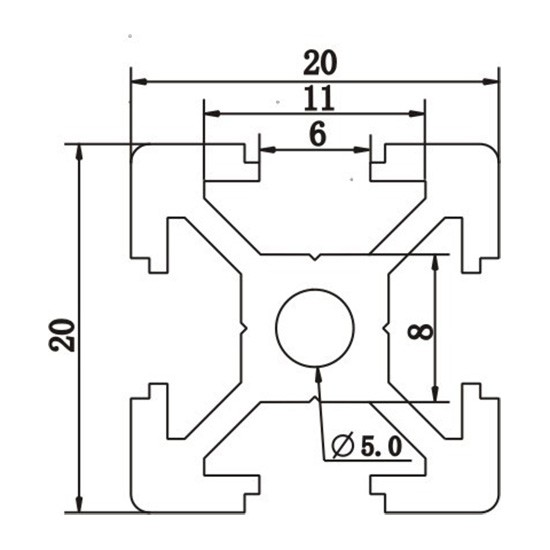
\includegraphics[width=0.3\linewidth]{2020}}
\subfigure{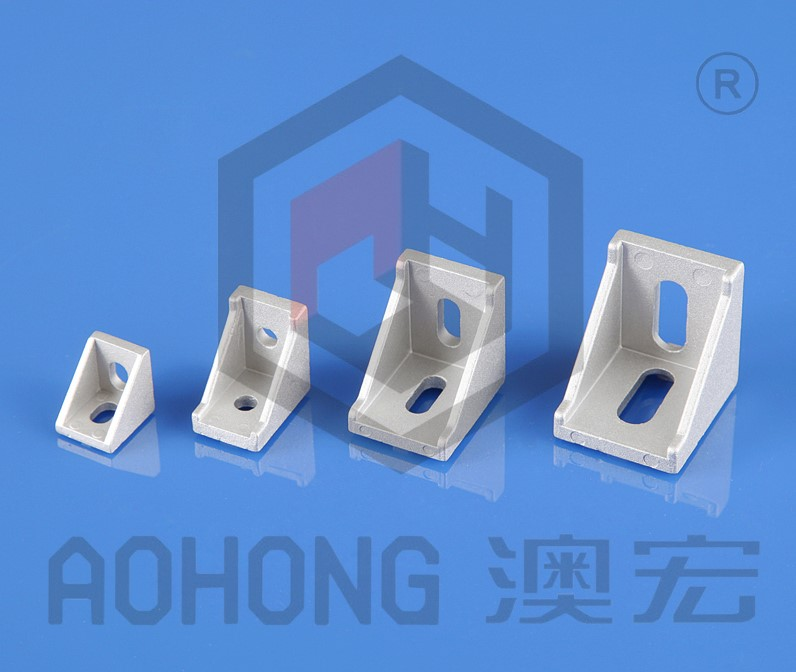
\includegraphics[width=0.29\linewidth]{Angled}}
\caption{(Left) The 2020 alumium extrusion.}
\caption{(Right) The angled iron for the extrusion.}
\end{figure}
\par On the front of the throwing part, we added an component that can limit the final position of the beam. The hole on the bottom part is for a M5 screw that attaches to one piece of alumium extrusion, and the rest of the $\phi 8$ holes are for limiting the position of the shaft that achieves this function.

\begin{figure}[H]
\centering
\subfigure{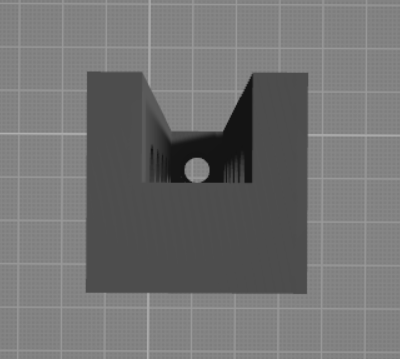
\includegraphics[width=0.39\linewidth]{SH1}}
\subfigure{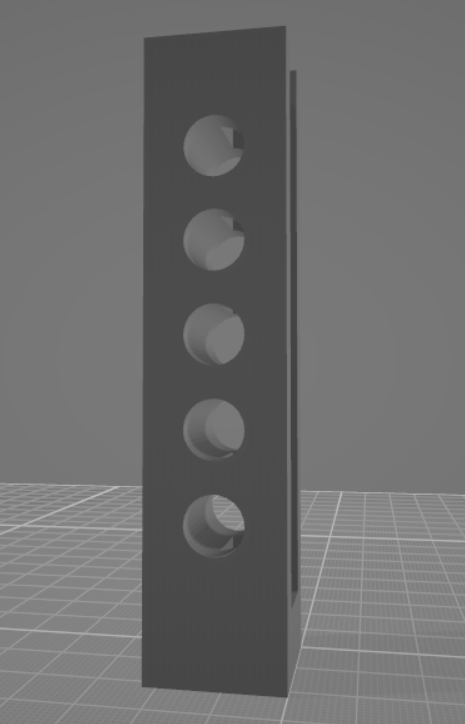
\includegraphics[width=0.223\linewidth]{SH2}}
\subfigure{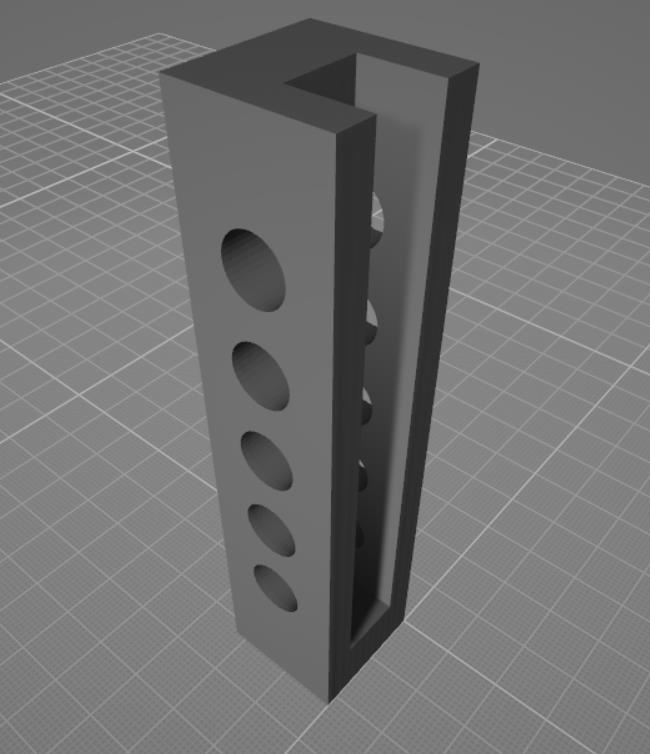
\includegraphics[width=0.3\linewidth]{SH3}}
\caption{Design concept of the limiting component.}
\end{figure}
~\\
\begin{figure}[H]
\centering
\subfigure{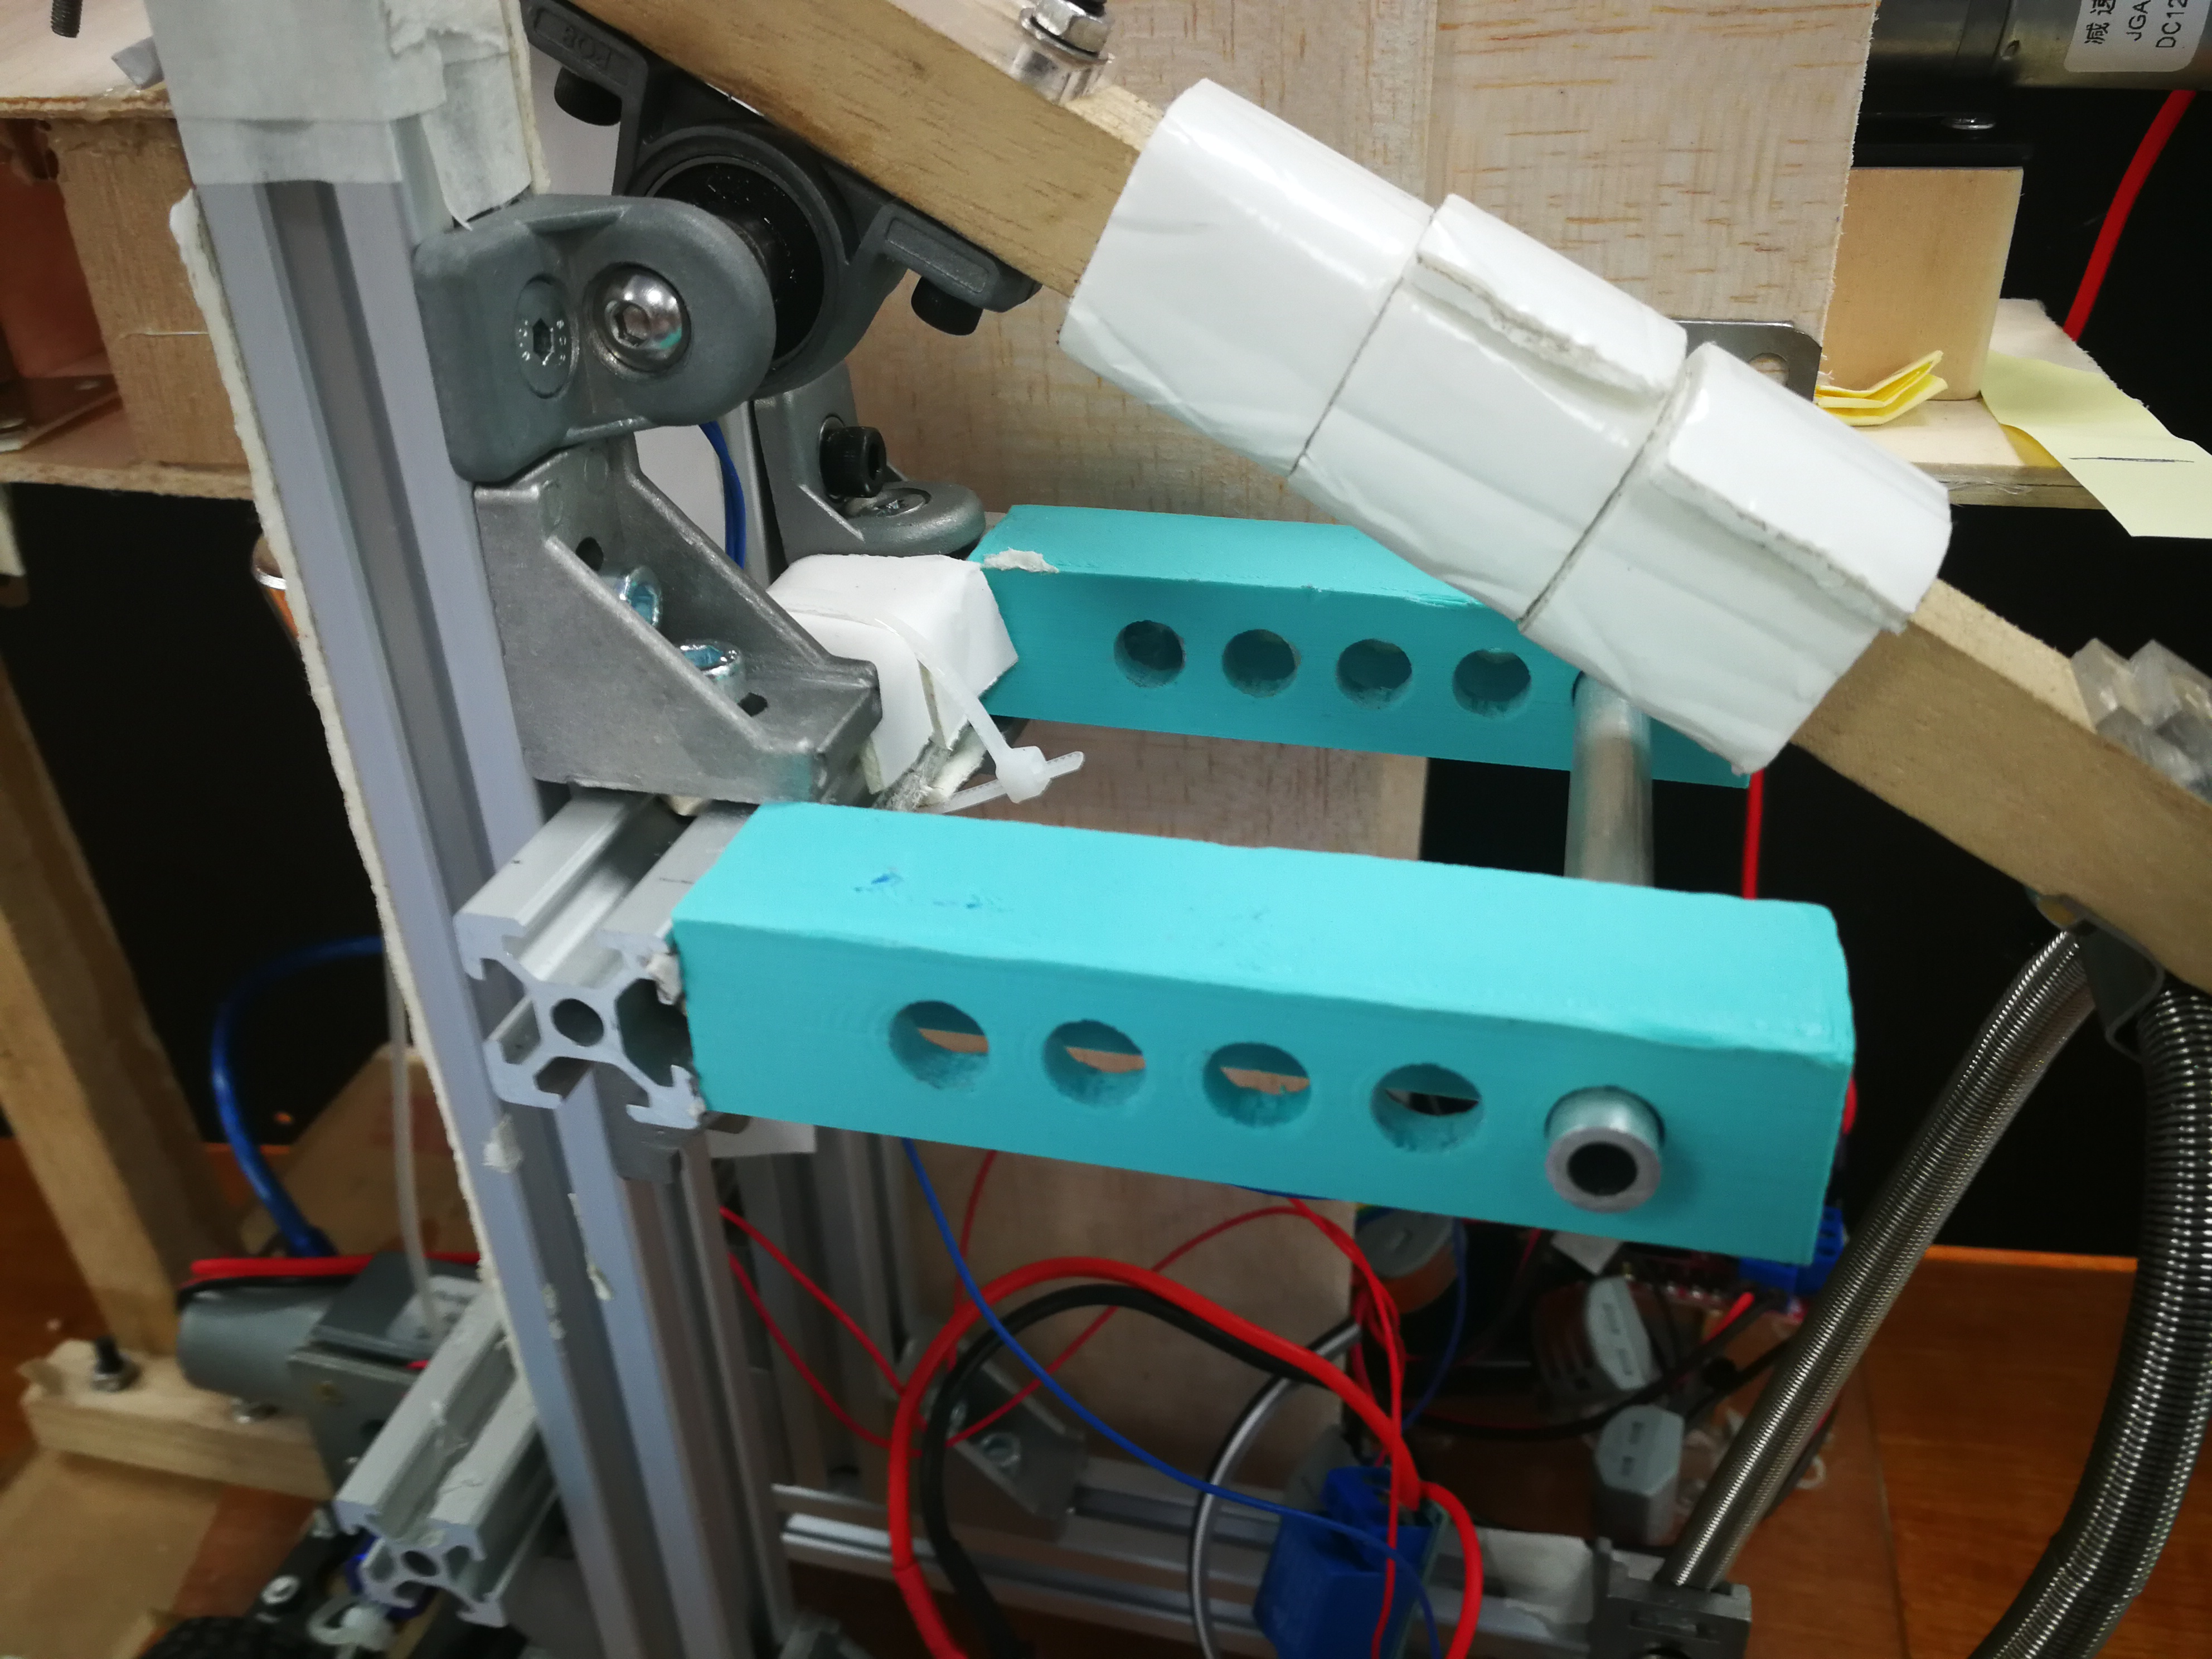
\includegraphics[width=0.5\linewidth]{Limit}}
\subfigure{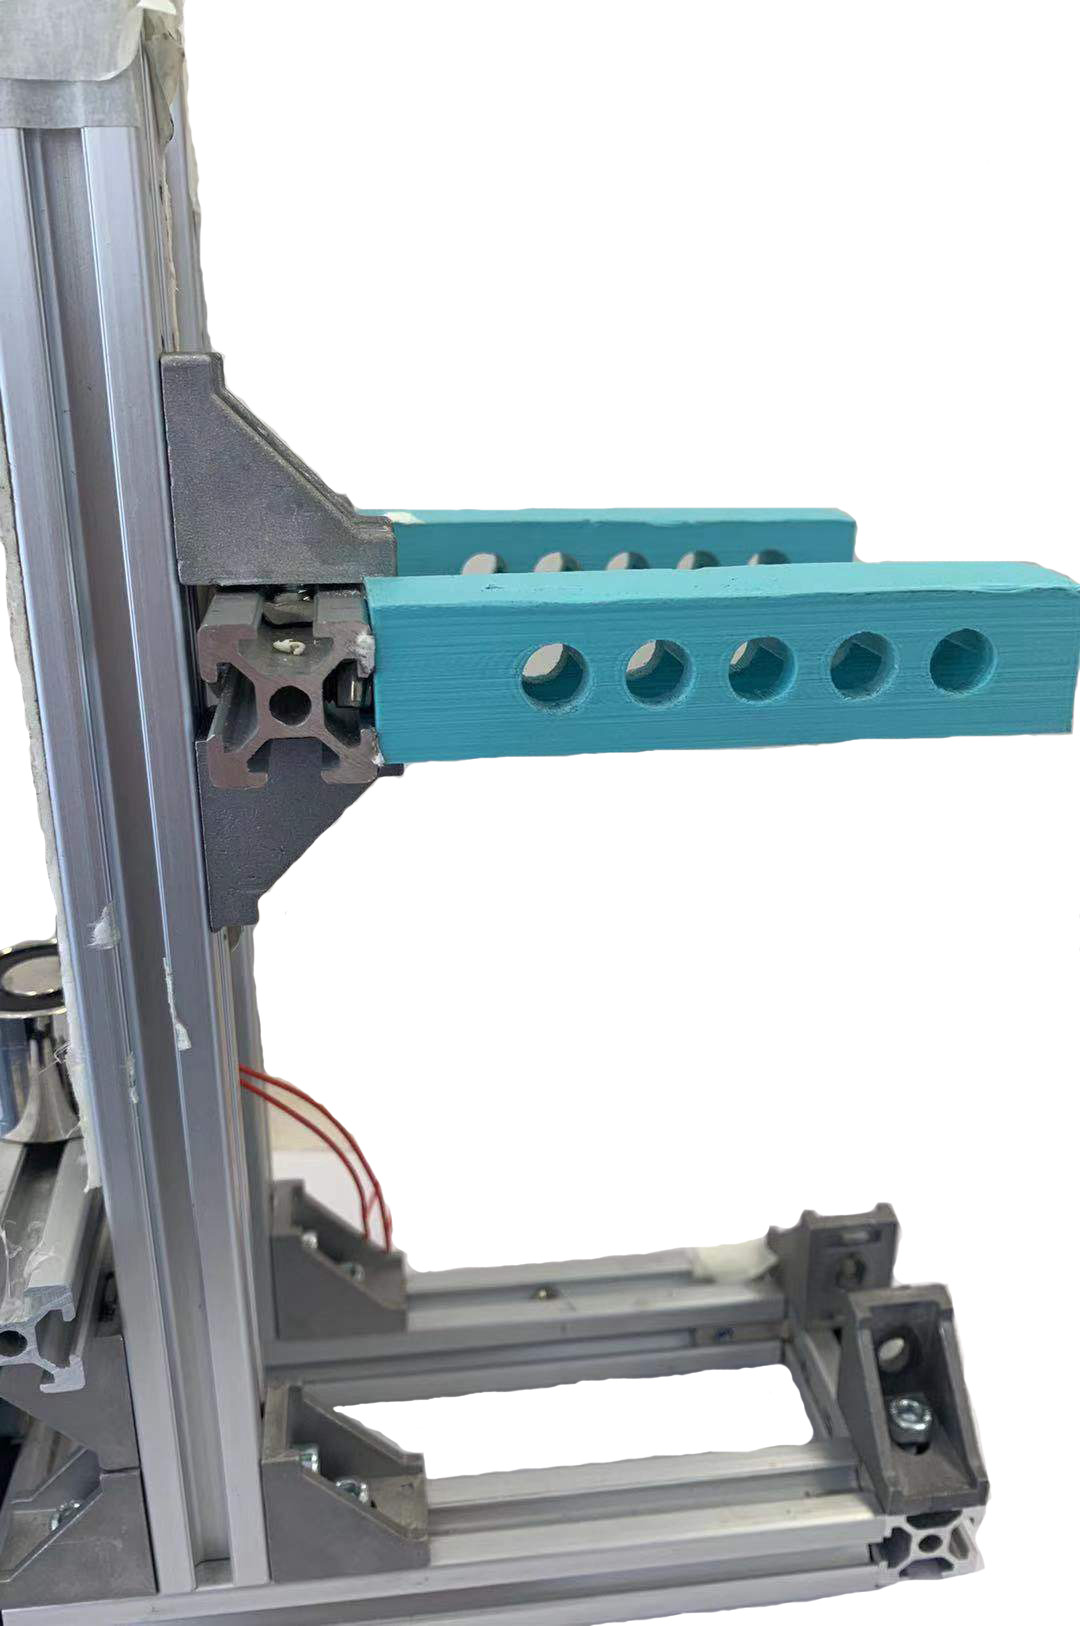
\includegraphics[width=0.3\linewidth]{6}}
\caption{The real application of limiting component.}
\end{figure}
~\\

\subsubsection*{Reloading Structure}
For the reloading, we used Archimedes' Screw to operate. By controlling the rotating direction of the screw, we could control the moving direction of the ball putting on it. When revolving, the friction existed on the contact area of the screw and the wooden board (used to support this structure). Therefore, we stuck a piece of acrylic onto the wooden board so that the friction can be minimized, and during the real operation, this structure goes well.

\begin{figure}[H]
\centering
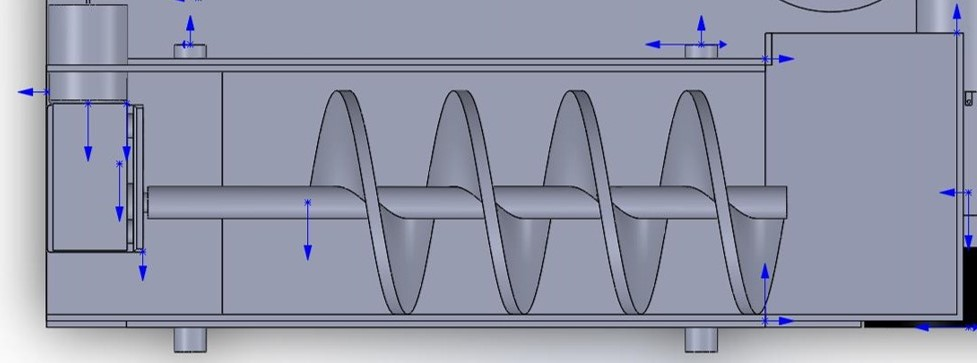
\includegraphics[width=0.6\linewidth]{Screw3}
\caption{Concept of the reloading structure.}
\end{figure}

\subsubsection*{Pugh Chart}



We compare the two models following:
\begin{figure}[H]
\centering
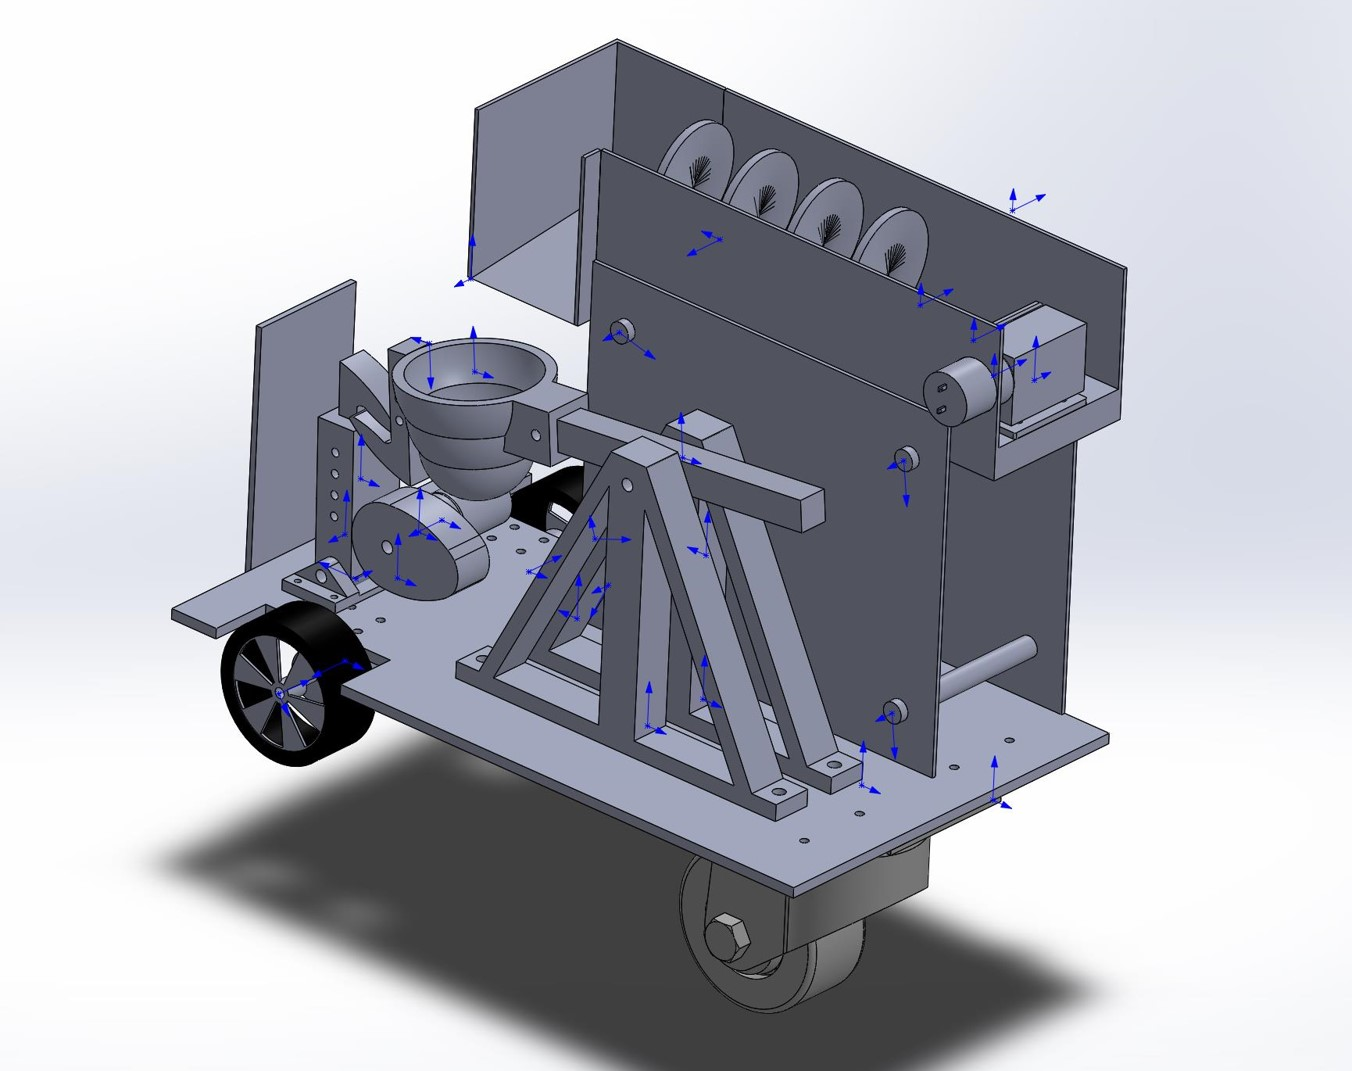
\includegraphics[width=0.6\linewidth]{Overall}
\caption{Concept 1: The final design concept.}
\end{figure}

\begin{figure}[H]
\centering
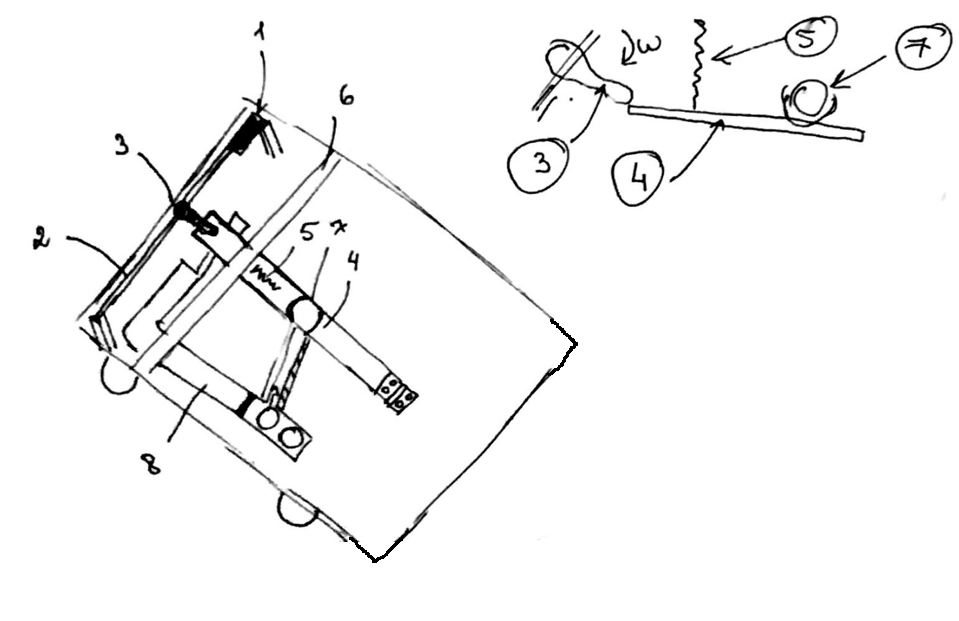
\includegraphics[width=0.6\linewidth]{Con1}
\caption{Concept 2: The original design concept.}
\end{figure}

\par Now use the Pugh Chart, we compare these two concepts in a quantitative approach.\\

% Table generated by Excel2LaTeX from sheet 'Sheet1'
\begin{table}[H]
\centering
\begin{tabular}{rrrr}
Requireents &     Weight &  Concept 1 &  Concept 2 \\
\hline
    Speed  &          4 &          S &          S \\

      Size &          8 &          S &          + \\

Reliability &          9 &          + &          S \\

      Cost &          5 &          + &          $-$ \\

  Accuracy &         10 &          S &          S \\

    Reload &          9 &          S &          S \\
\hline
\multicolumn{ 1}{c}{} &    Total $+$ &         14 &          8 \\

\multicolumn{ 1}{c}{} &    Total $-$ &          0 &          5 \\

\multicolumn{ 1}{c}{} &      Total &         14 &         3 \\
\end{tabular} 
\caption{Pugh chart.}
\end{table}

\par From the Pugh chart, we can clearly see that the concept 1 is much better than the concept 2. Therefore, we followed the concept 1 to manufacture our car.


\subsection{Embodiment Design}
\subsubsection*{Material Chosen}
\par Material choice is quite important towards the final prototype, as different materials show different requirements on tolerance, stability and weight. The different materials are analyzed as follows:

% Table generated by Excel2LaTeX from sheet 'Sheet1'
\begin{table}[H]
\centering
\begin{tabular}{r|rrr}
           &    Acrylic &   Aluminum &       Wood \\
\hline
   Density &        $++$ &        $+++$ &      $+$ \\

Tensile strength &         $++$ &         $+++$ &         $+$ \\

     Price &        $++$ &        $+++$ &        $+$ \\

Difficulty in processing &          ++ &          +++ &          + \\
\end{tabular} 
\caption{The effective property of the three chosen materials.}

\end{table}
 


\subsubsection*{Chassis}
The main requirements for choosing the right material for our chassis depended on strength and durability. Material options our team considered included aluminum metal, wood and acrylic board. Although wood is a very easy material to manufacture, it is too light that it's unsuitable for withstanding constant impact forces. Similarly, aluminum metal is a strong material but easily malleable. This metal characteristic makes aluminum metal prone to deformation. Therefore, our team choose to use an acrylic board. Acrylic material properties include rigidity, good impact strength and toughness. The Acrylic material was laser cut to the shape of our base.  The Acrylic base dimensions are $35cm\times 20cm\times 6mm (thickness) $

\begin{figure}[H]
\centering
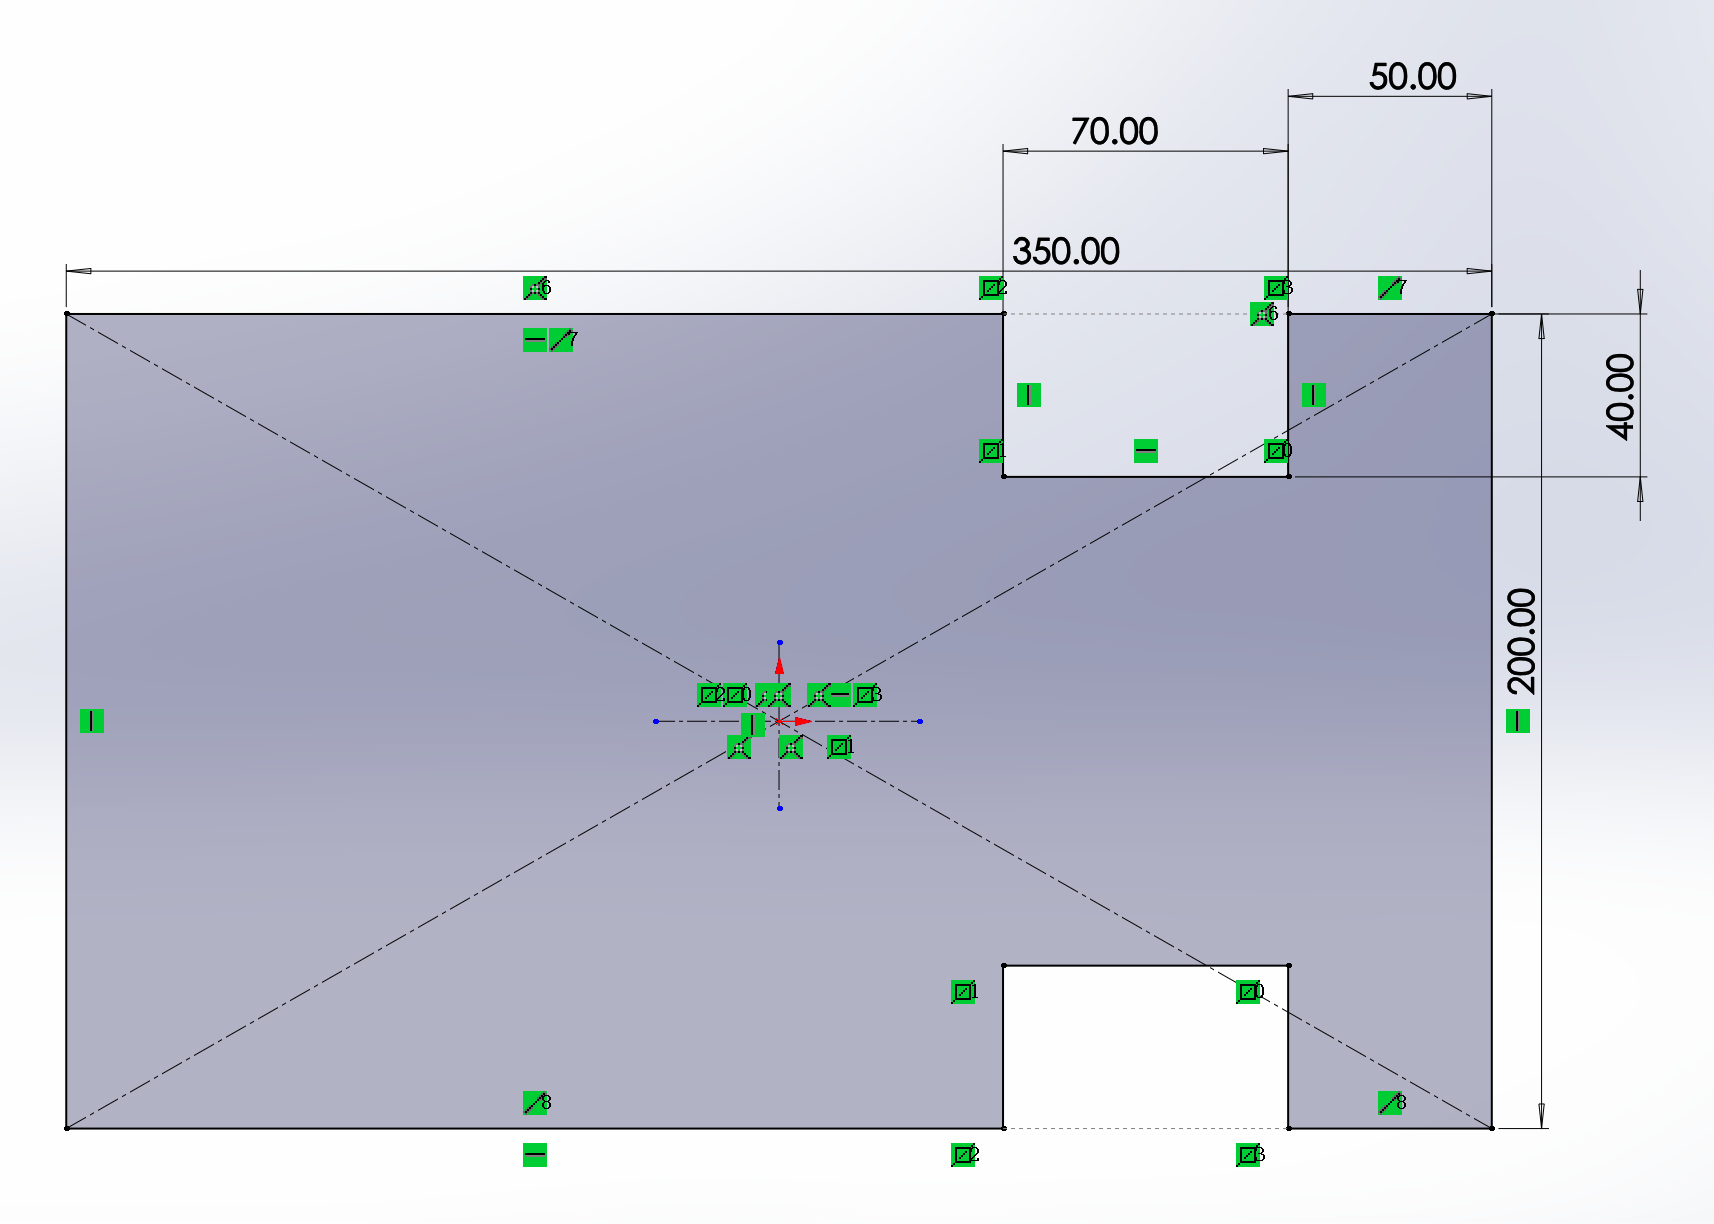
\includegraphics[width=0.6\linewidth]{board1}
\caption{The CAD design of the acrylic board.}
\end{figure}

\subsubsection*{Moving System}
Our team used rear driven system for our vehicle. Hence, two rear wheels are driven by two DC motors, one motor for each wheel. The motor-wheel system is mounted on the Acrylic base using iron angle plates fastened with screws. These wheels elevate the base 5 cm from the ground. Regarding the front wheels, two caster wheels are fixed to the base and are aligned perfectly with the back wheels
\begin{figure}[H]
\centering
\includegraphics[width=0.6\linewidth]{Moving}
\caption{The CAD design of the moving component.}
\end{figure}

\subsubsection*{Automatic Reloading System}
A 3-D printed Archimedes screw (PLA) powered by a DC motor provides the necessary motion to transport ping-pong and tennis balls towards the trebuchet basket. To accomplish this, a supporting system will be made from wood to elevate the Archimedes screw to the proper height of 35 cm from the floor. To hold the screw, we design a three-wall wooden box to hold this section, and at the edge of this box, we plan to add an angled ramp was included to help navigate the balls towards the trebuchet basket. This ramp is surrounded by wooden walls to prevent any ball from falling over.

\begin{figure}[H]
\centering
\subfigure{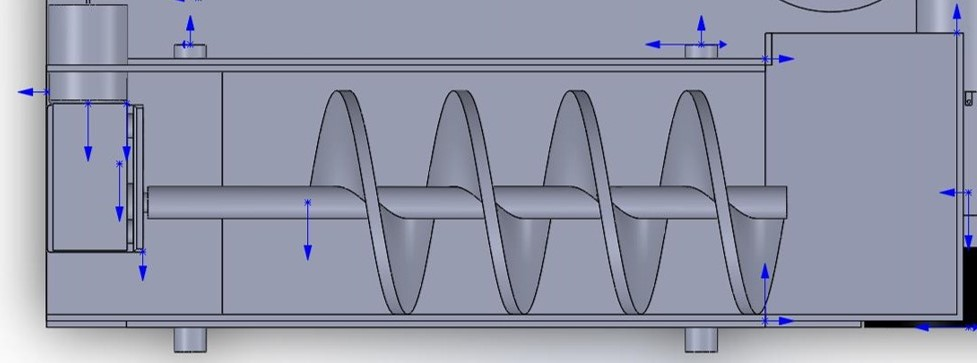
\includegraphics[width=0.5\linewidth]{Screw3}}
\subfigure{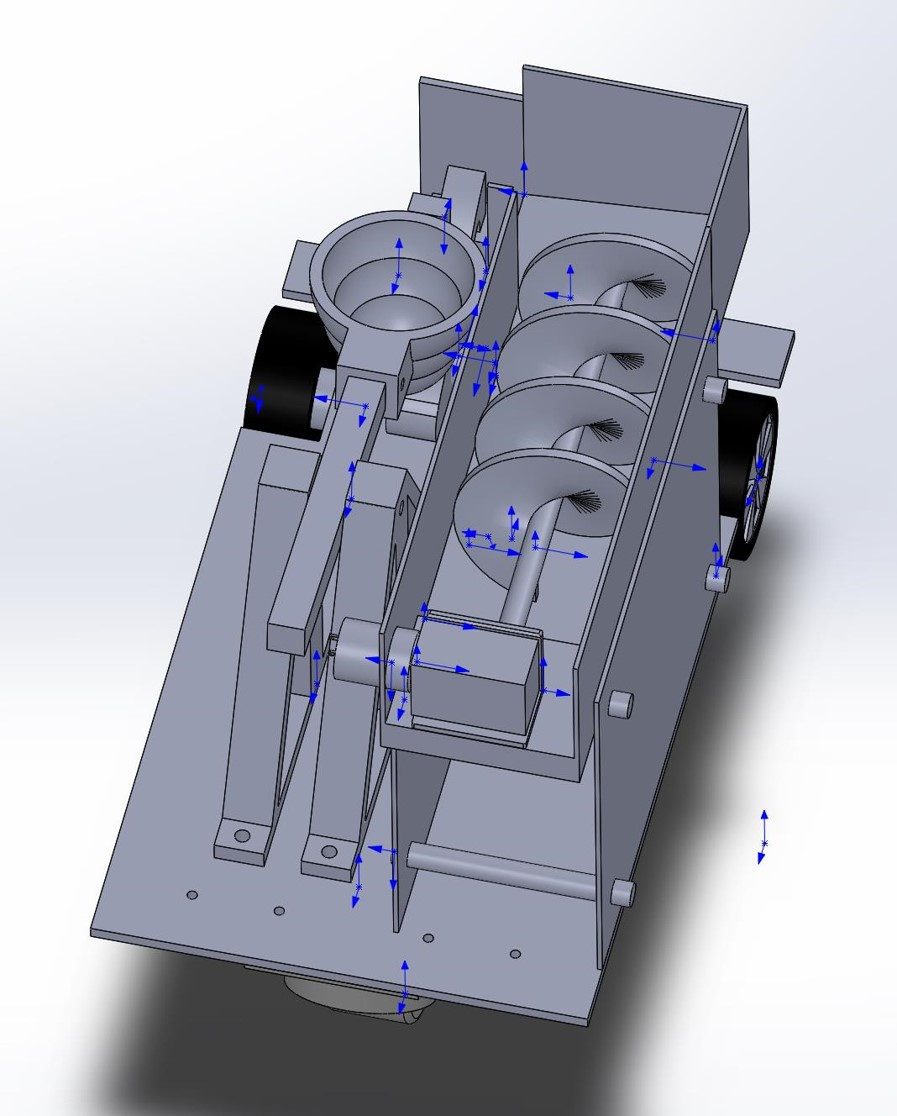
\includegraphics[width=0.3\linewidth]{Up2}}
\caption{The CAD design for the reloading component.}
\end{figure}

\subsubsection*{Shooting System}
The shooting part is separated into the shooting beam part and the base part. For the beam part, this has been discussed in the go/on-go screening section. For the shooting base part, our aim for this is that it can elevate the shooting beam to the desired hight, which will tested in order to get the perfect shooting distance, and ensure the stability of the whole structure. We plan to use the 2020 alumium extrusion to achieve this, and the diagram for fixing them together is shown below.

\begin{figure}[H]
\centering
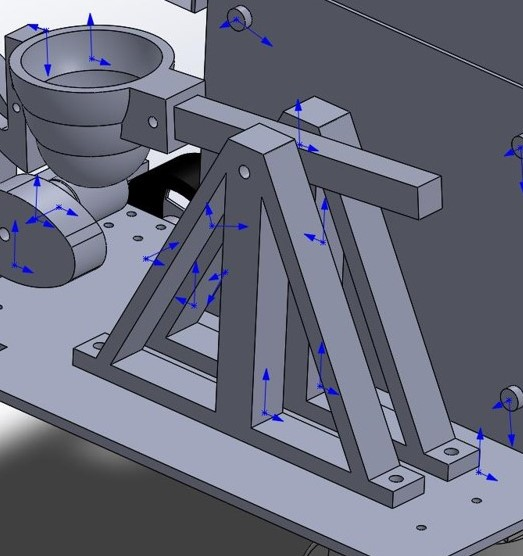
\includegraphics[width=0.5\linewidth]{Stand1}
\caption{The CAD design for the shooting system.}
\end{figure}

\subsubsection*{Remote Control System}
We use PS2 joystick as the remote controller and assign the following bottoms to proceed each kind of work:\\
\begin{itemize}
\item Right: Start reloading.
\item Left: Reverse reloading process.
\item Up: Loose the string.
\item Down: Tighten the sring
\item L3: Fix the bar.
\item R3: Loose the bar.
\item L2: Stop reloading.
\item R2: Stop the car.
\item Triangle: Go straight.
\item Circle: Turn right.
\item Cross: Go back.
\item Square: Turn left.
\end{itemize}

\begin{figure}[H]
\centering
\subfigure{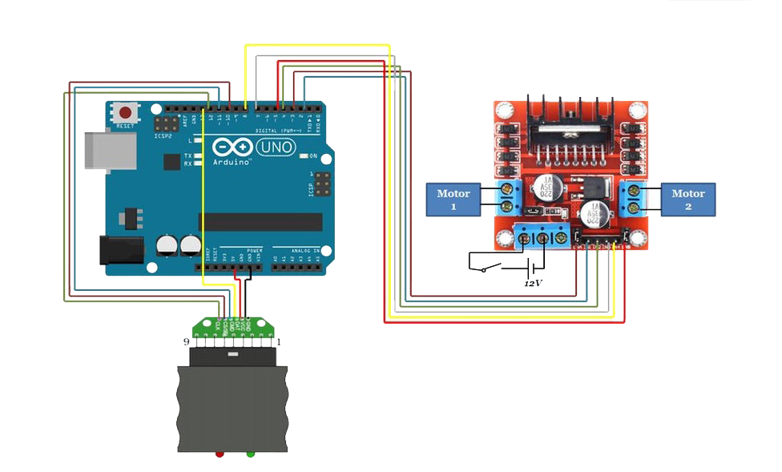
\includegraphics[width=0.55\linewidth]{circuit}}
\subfigure{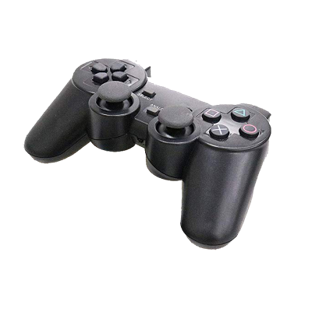
\includegraphics[width=0.3\linewidth]{ps2}}
\caption{The circuit design for the remote control system(motors).}
\end{figure}


\subsubsection*{Trebuchet arm and Basket}
The trebuchet arm, $30cm\times 1.5cm\times 1.5cm$, is made from wood to enable flexibility. The basket was 3-D printed using PLA. The basket design enables a portion of the arm to be inserted inside and then the basket is fixed to the arm by screws. The design of the basket allows ping-pong, racket, tennis balls to be slightly grip for each different size.  An additional 3-D printed part is fixed to the arm, just to the right of the basket to enable different rope and wire to easily wrap around the arm.
\begin{figure}[H]
\centering
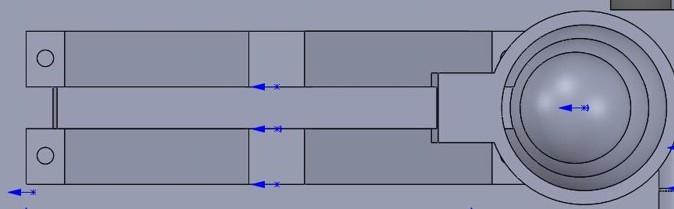
\includegraphics[width=0.5\linewidth]{arm}
\caption{The CAD design for the trebuchet arm and Basket.}
\end{figure}
\
\
%=========================
%
%
\section{Manufacturing}
\subsection{Prototype}
\subsubsection*{Chassis}
Following is the CAD of our acrylic board, the board we ordered online is $35cm\times 20cm\times 6mm $ and the cutting follows the CAD design in Section 3.3. For the rest of the holes needed to support the guiding wheels, motors, trebuchet holder, ect, we used the bench drill in JI lab to achieve our requirements for the position of them. 

\begin{figure}[H]
\centering
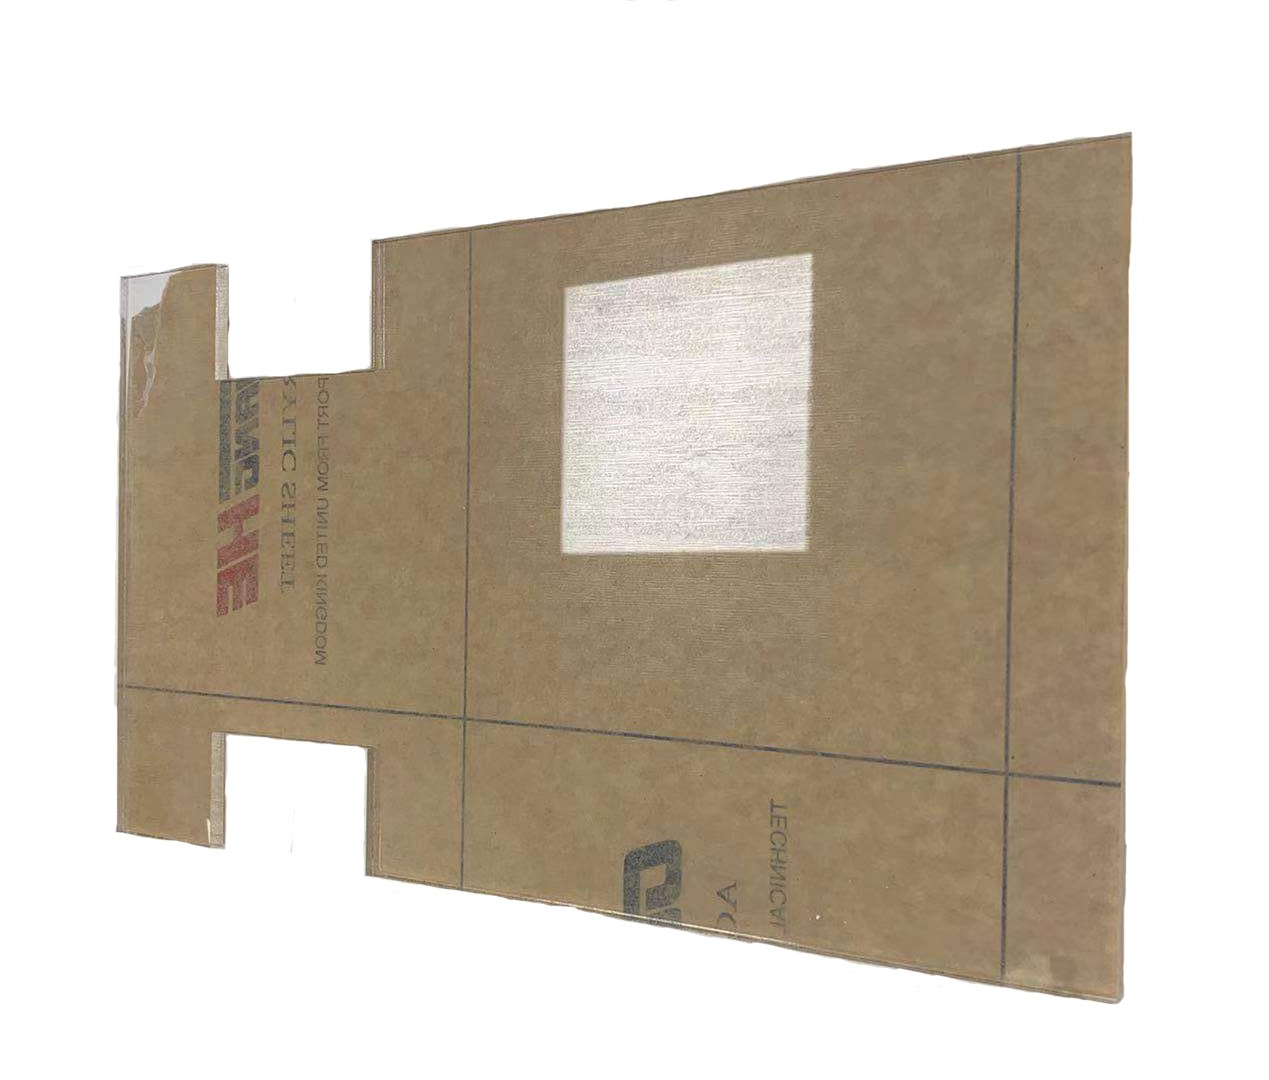
\includegraphics[width=0.4\linewidth]{5}
\caption{The online ordered chassis.}
\end{figure}


\subsubsection*{Moving System}
Two rear wheels are driven by two DC motors, one motor for each wheel. The motor-wheel system is mounted on the Acrylic base using iron angle plates fastened with screws. These wheels elevate the base 5 cm from the ground. The motors are connected to L298N driving board, which enables the controlling and the operating of this system.
\begin{figure}[H]
\centering
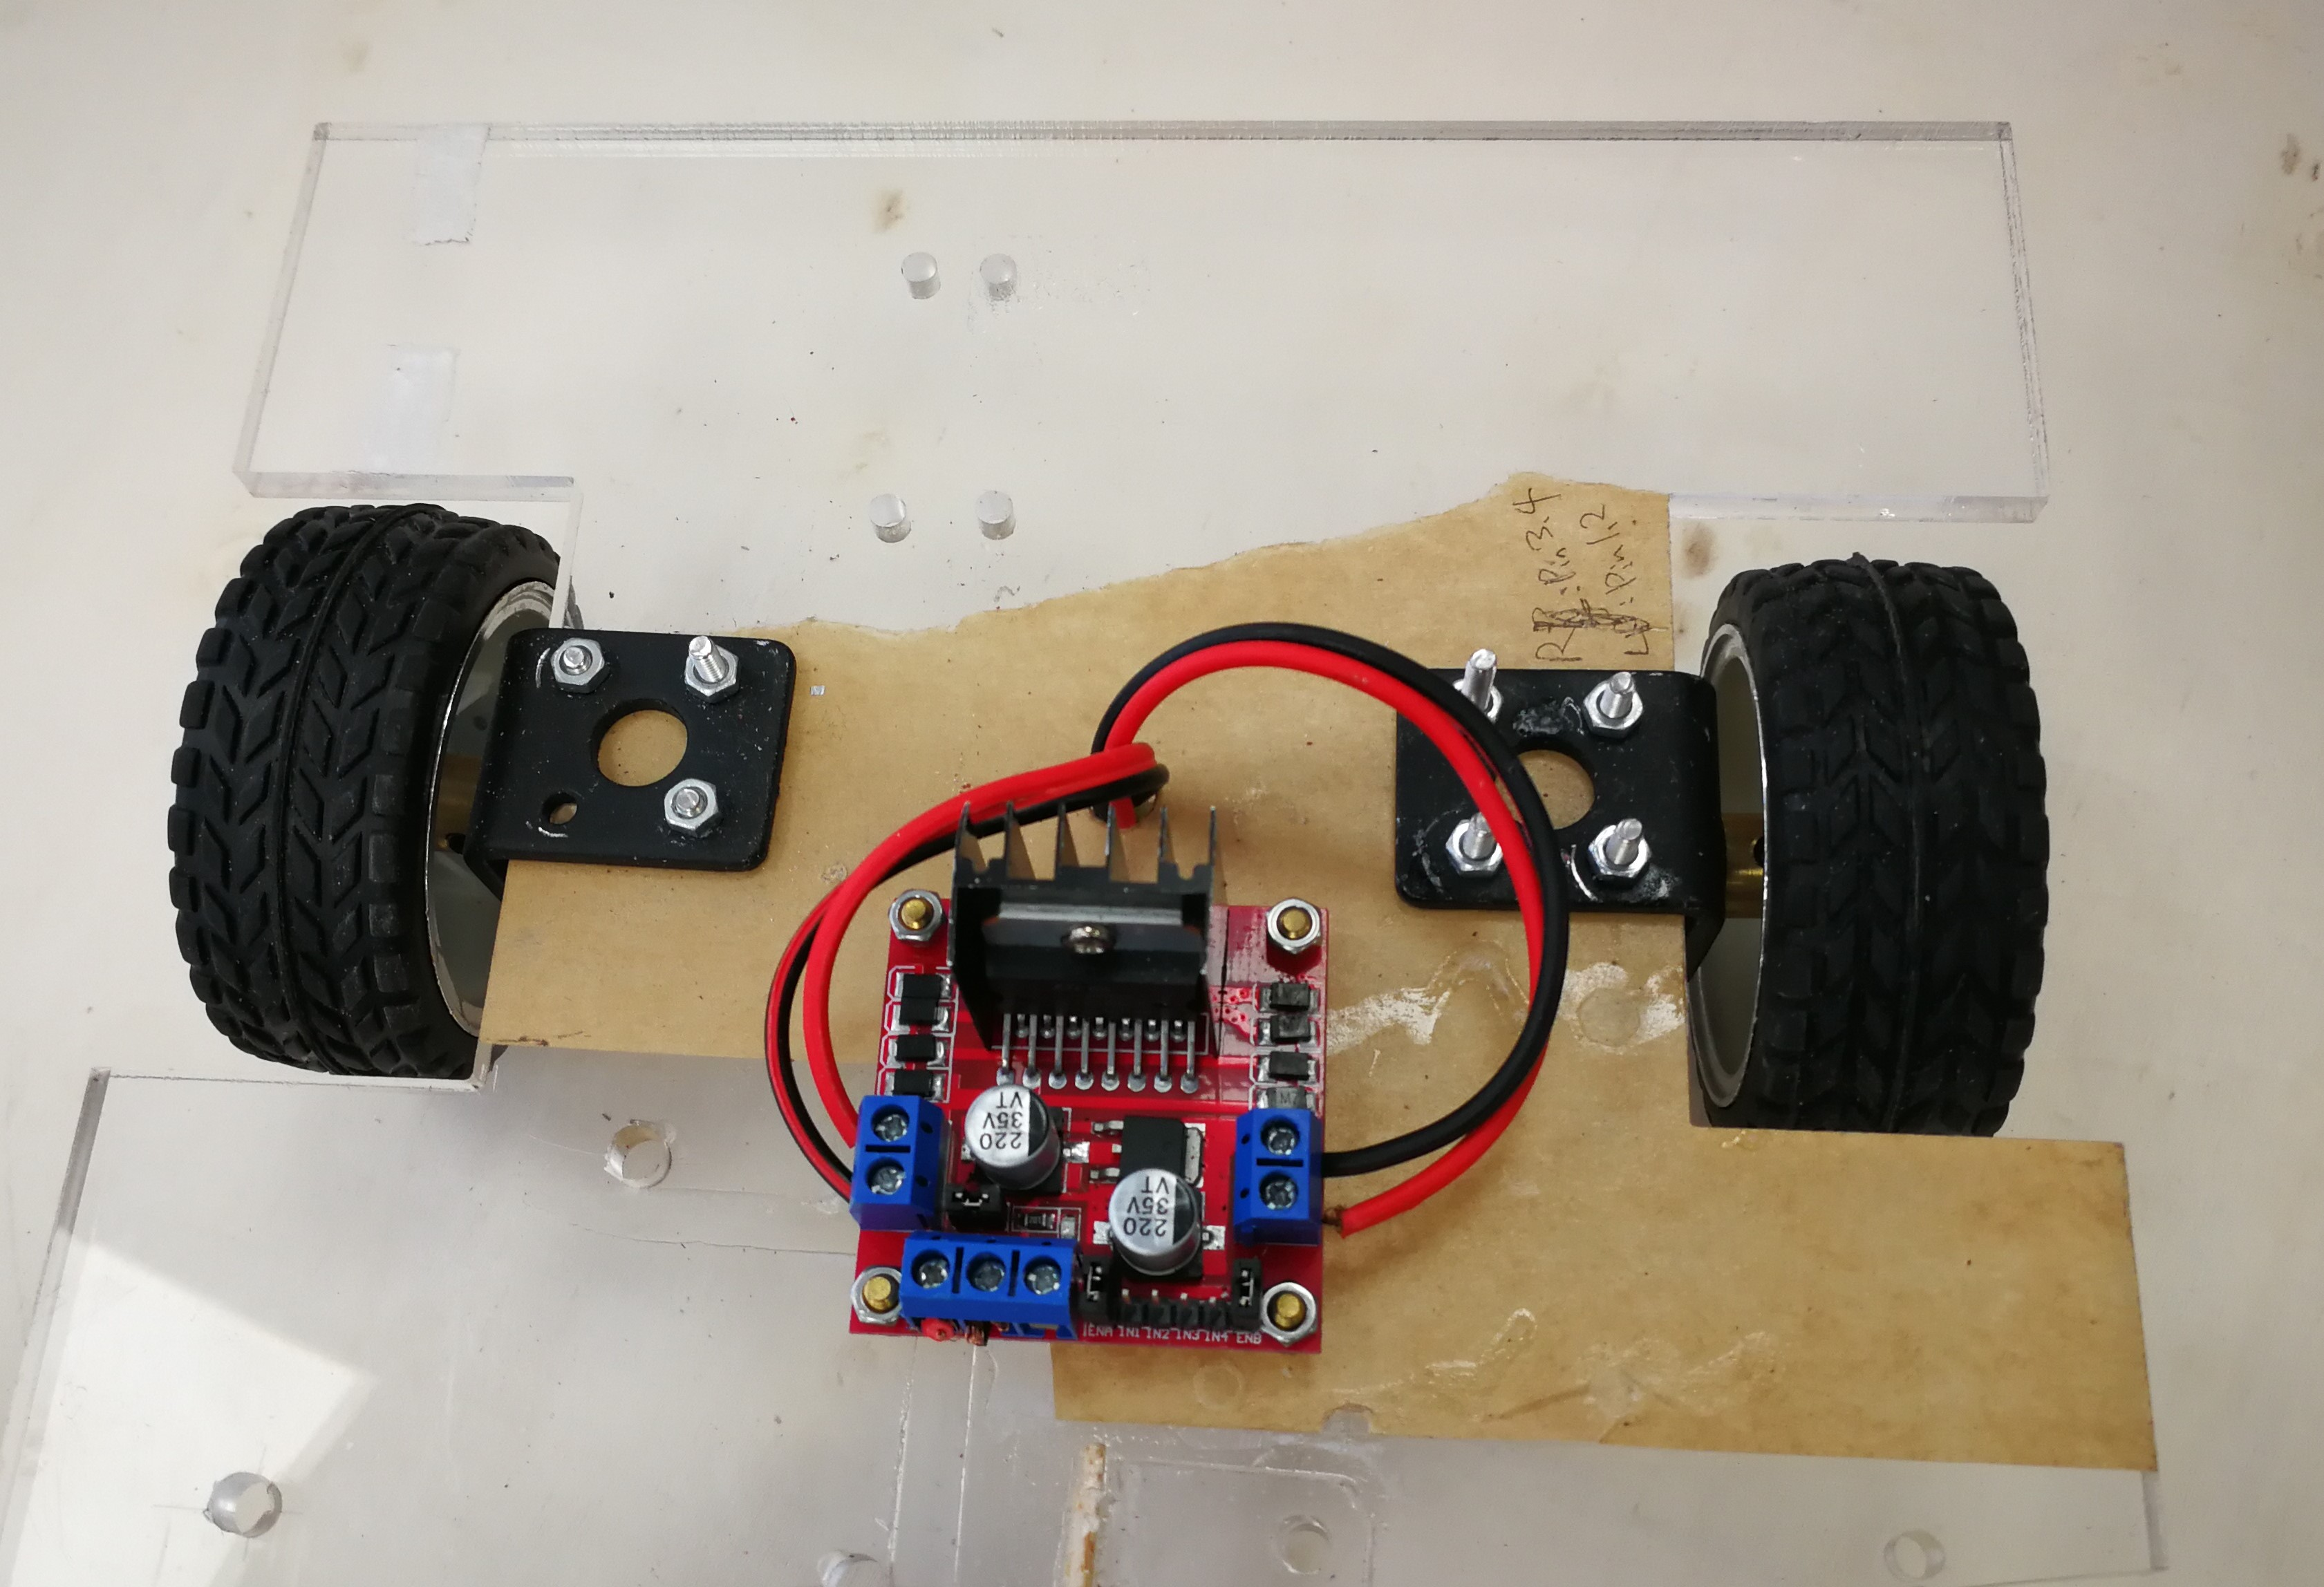
\includegraphics[width=0.5\linewidth]{wheel1}
\caption{The formation of the rear wheels.}
\end{figure}

For the front wheels, two caster wheels are fixed to the base and are aligned perfectly with the rear wheels. They work as the support for the whole body, and guides the movement of the car.
\begin{figure}[H]
\centering
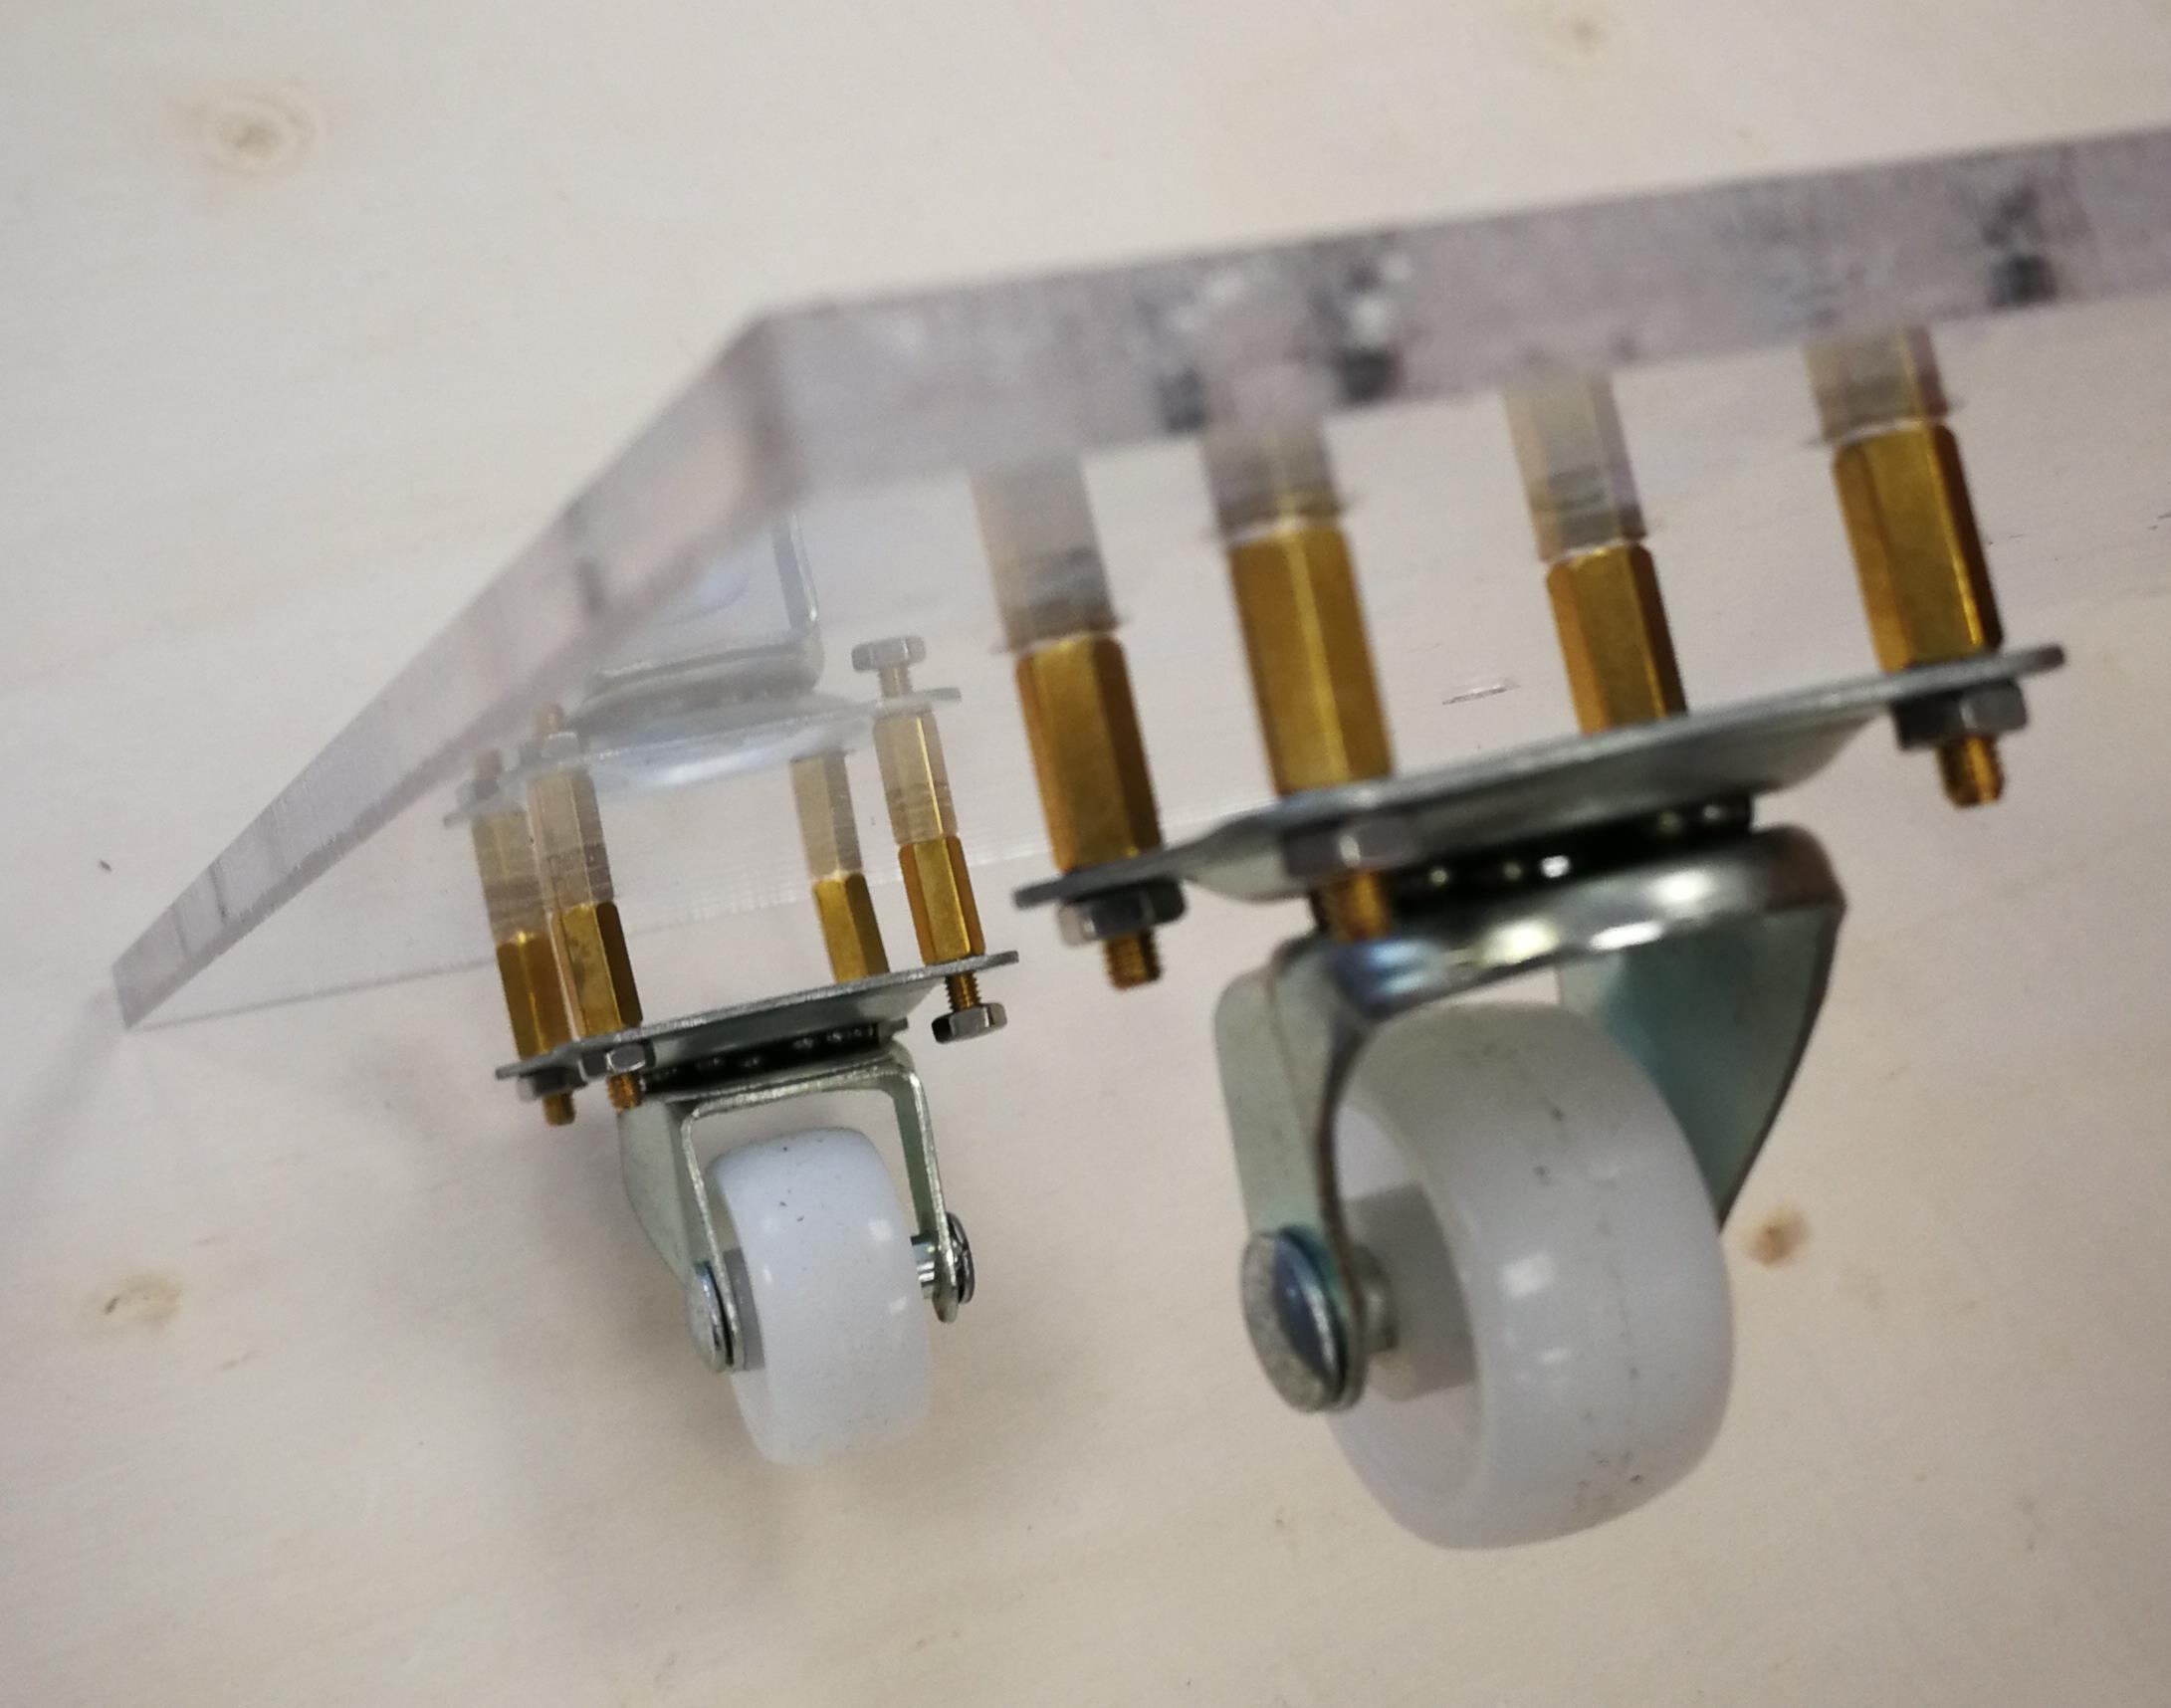
\includegraphics[width=0.5\linewidth]{wheel2}
\caption{The formation of the front wheels.}
\end{figure}



\subsubsection*{Automatic Reloading System}
A 3-D printed Archimedes screw (PLA) powered by a DC motor provides the necessary motion to transport ping-pong and tennis balls towards the trebuchet basket. A wooden frame was manufactured according to our CAD design. However, we found that a small portion of the Archimedes screw still touches the bottom wood due to bending in the spring coupler. To minimize friction, Acrylic material was glued to the bottom wood since Acrylic material has a lower coefficient of friction.
\begin{figure}[H]
\centering
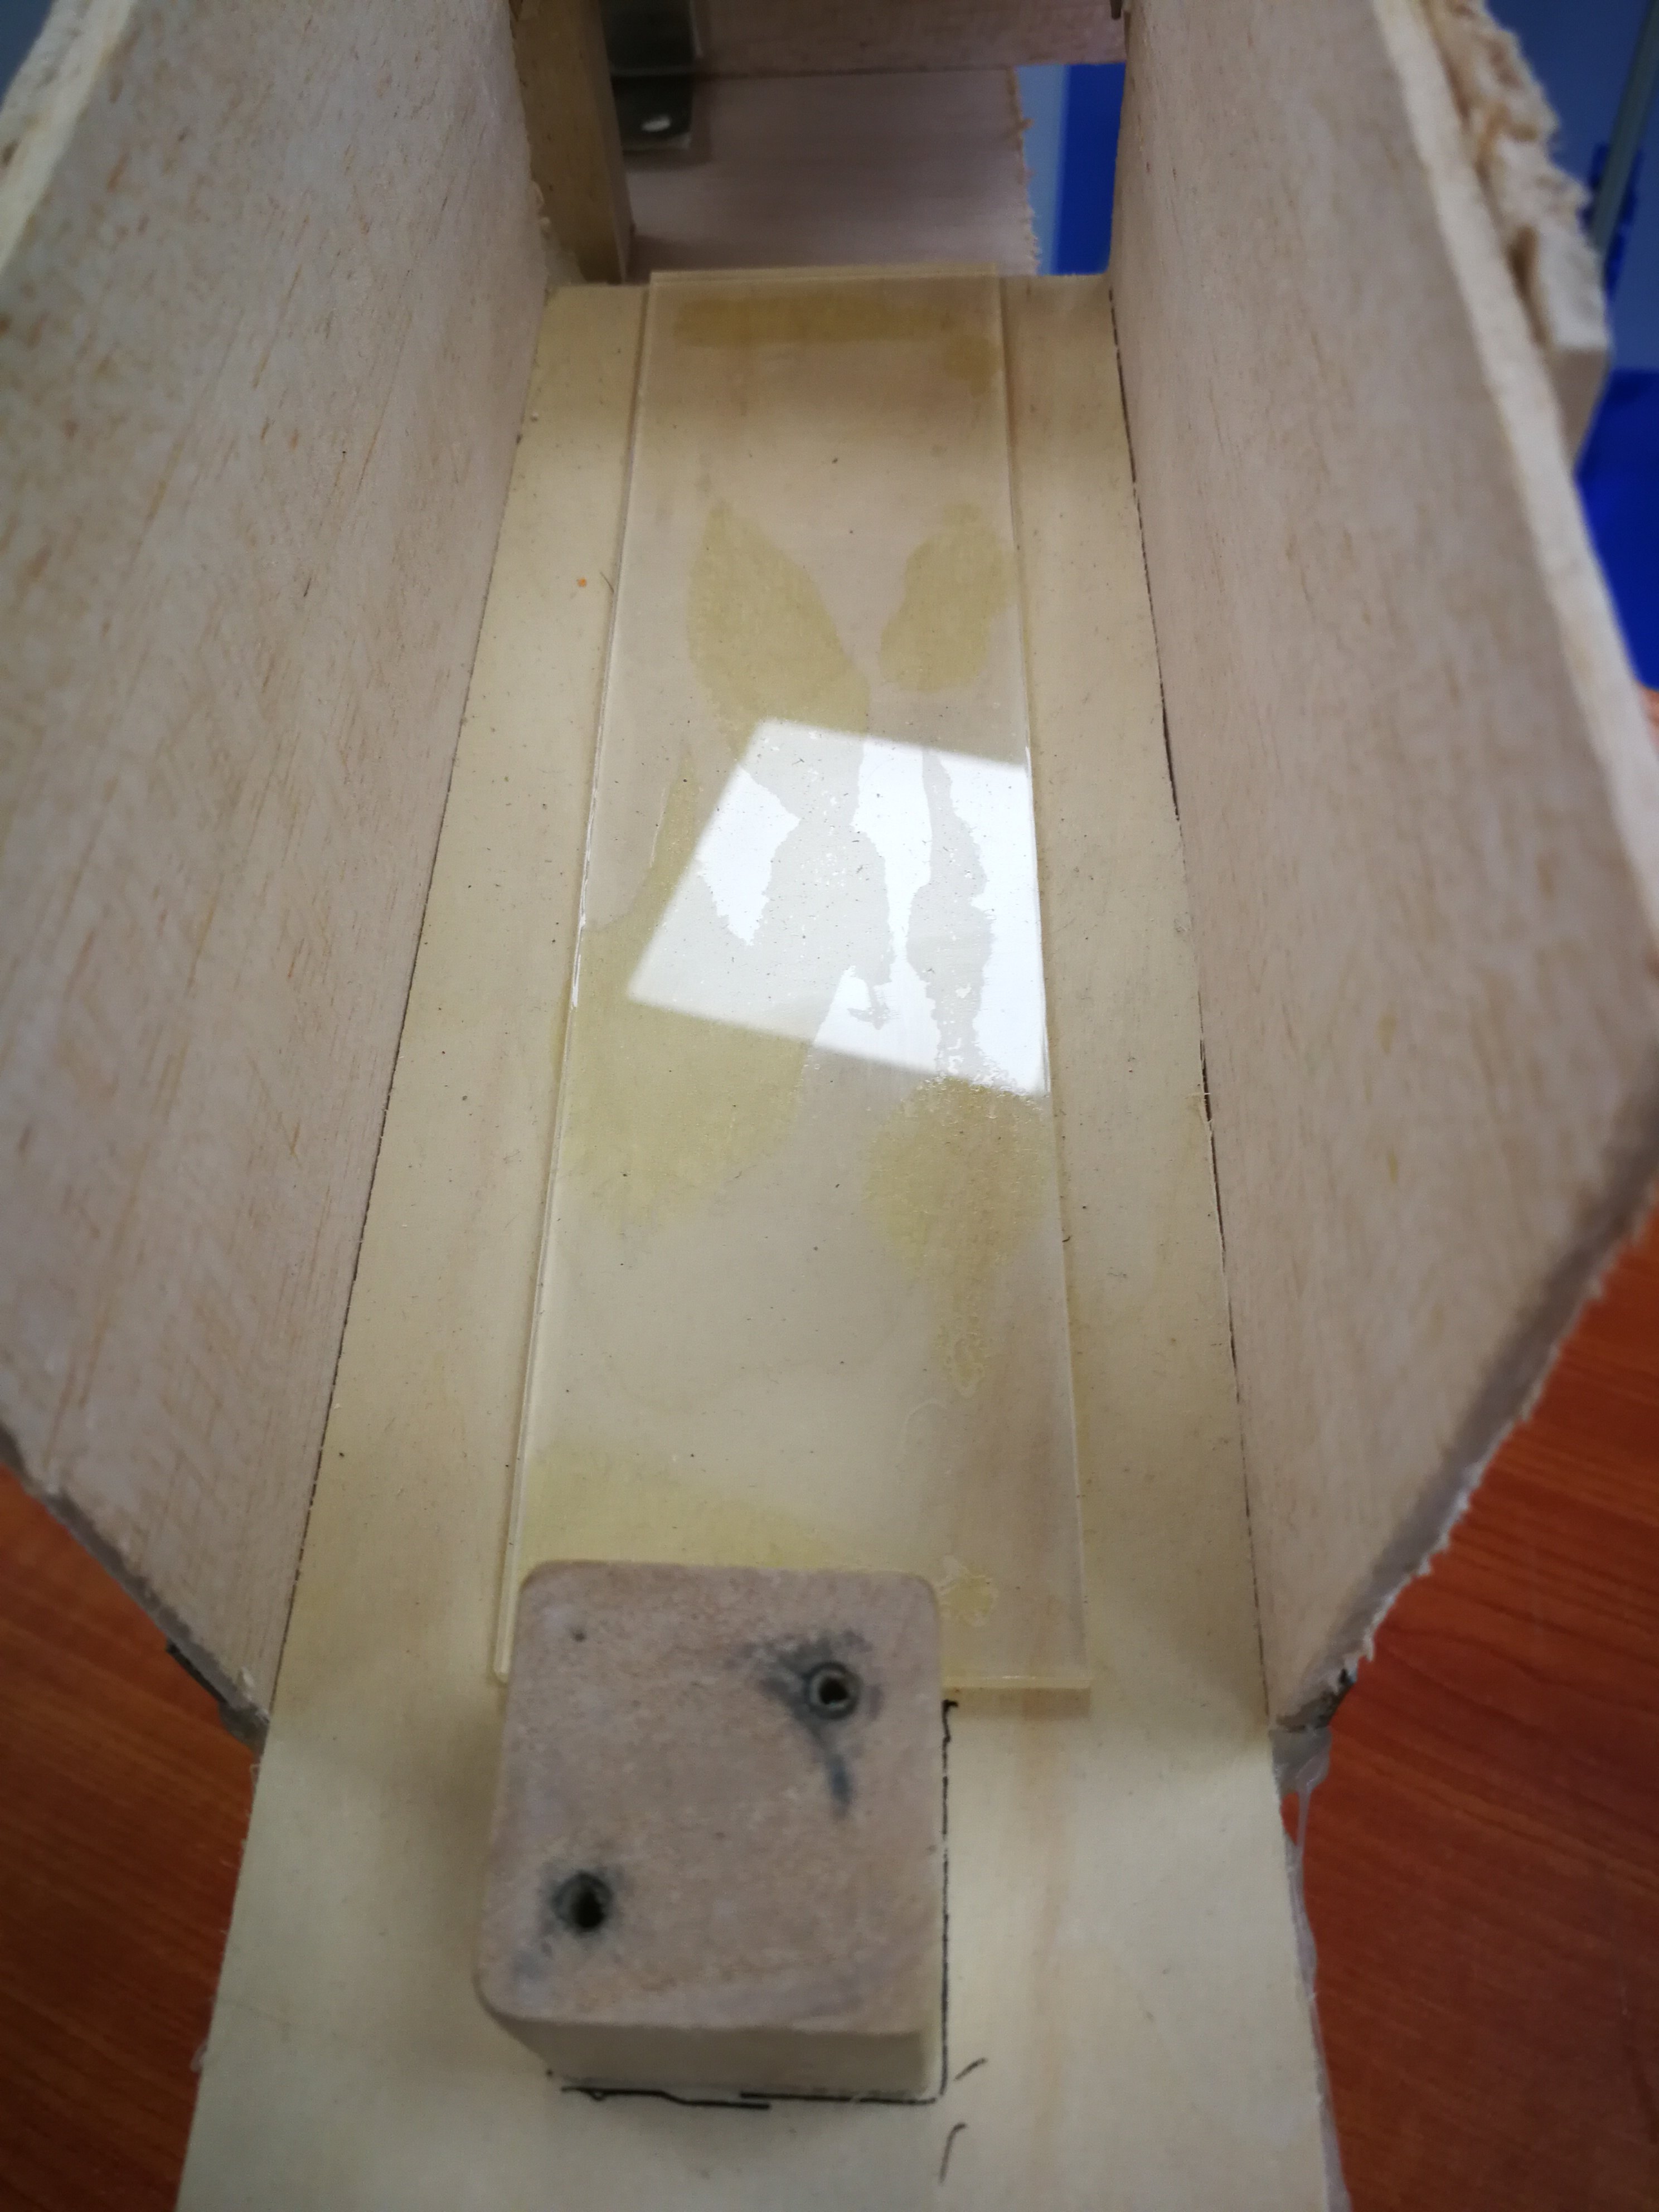
\includegraphics[width=0.4\linewidth]{stick}
\caption{Support box with glued acrylic board.}
\end{figure}

Towards the tip of the Archimedes screw, an angled ramp was included to help navigate the balls towards the trebuchet basket. This ramp is surrounded by wooden walls to prevent any ball from falling over. Furthermore, a 11 cm long, 4mm thick, plastic rod was glued perpendicular to the motion of the balls, in front of the Archimedes screw tip to give the balls a push towards the ramp. All these components form the automatic reloading system.
\begin{figure}[H]
\centering
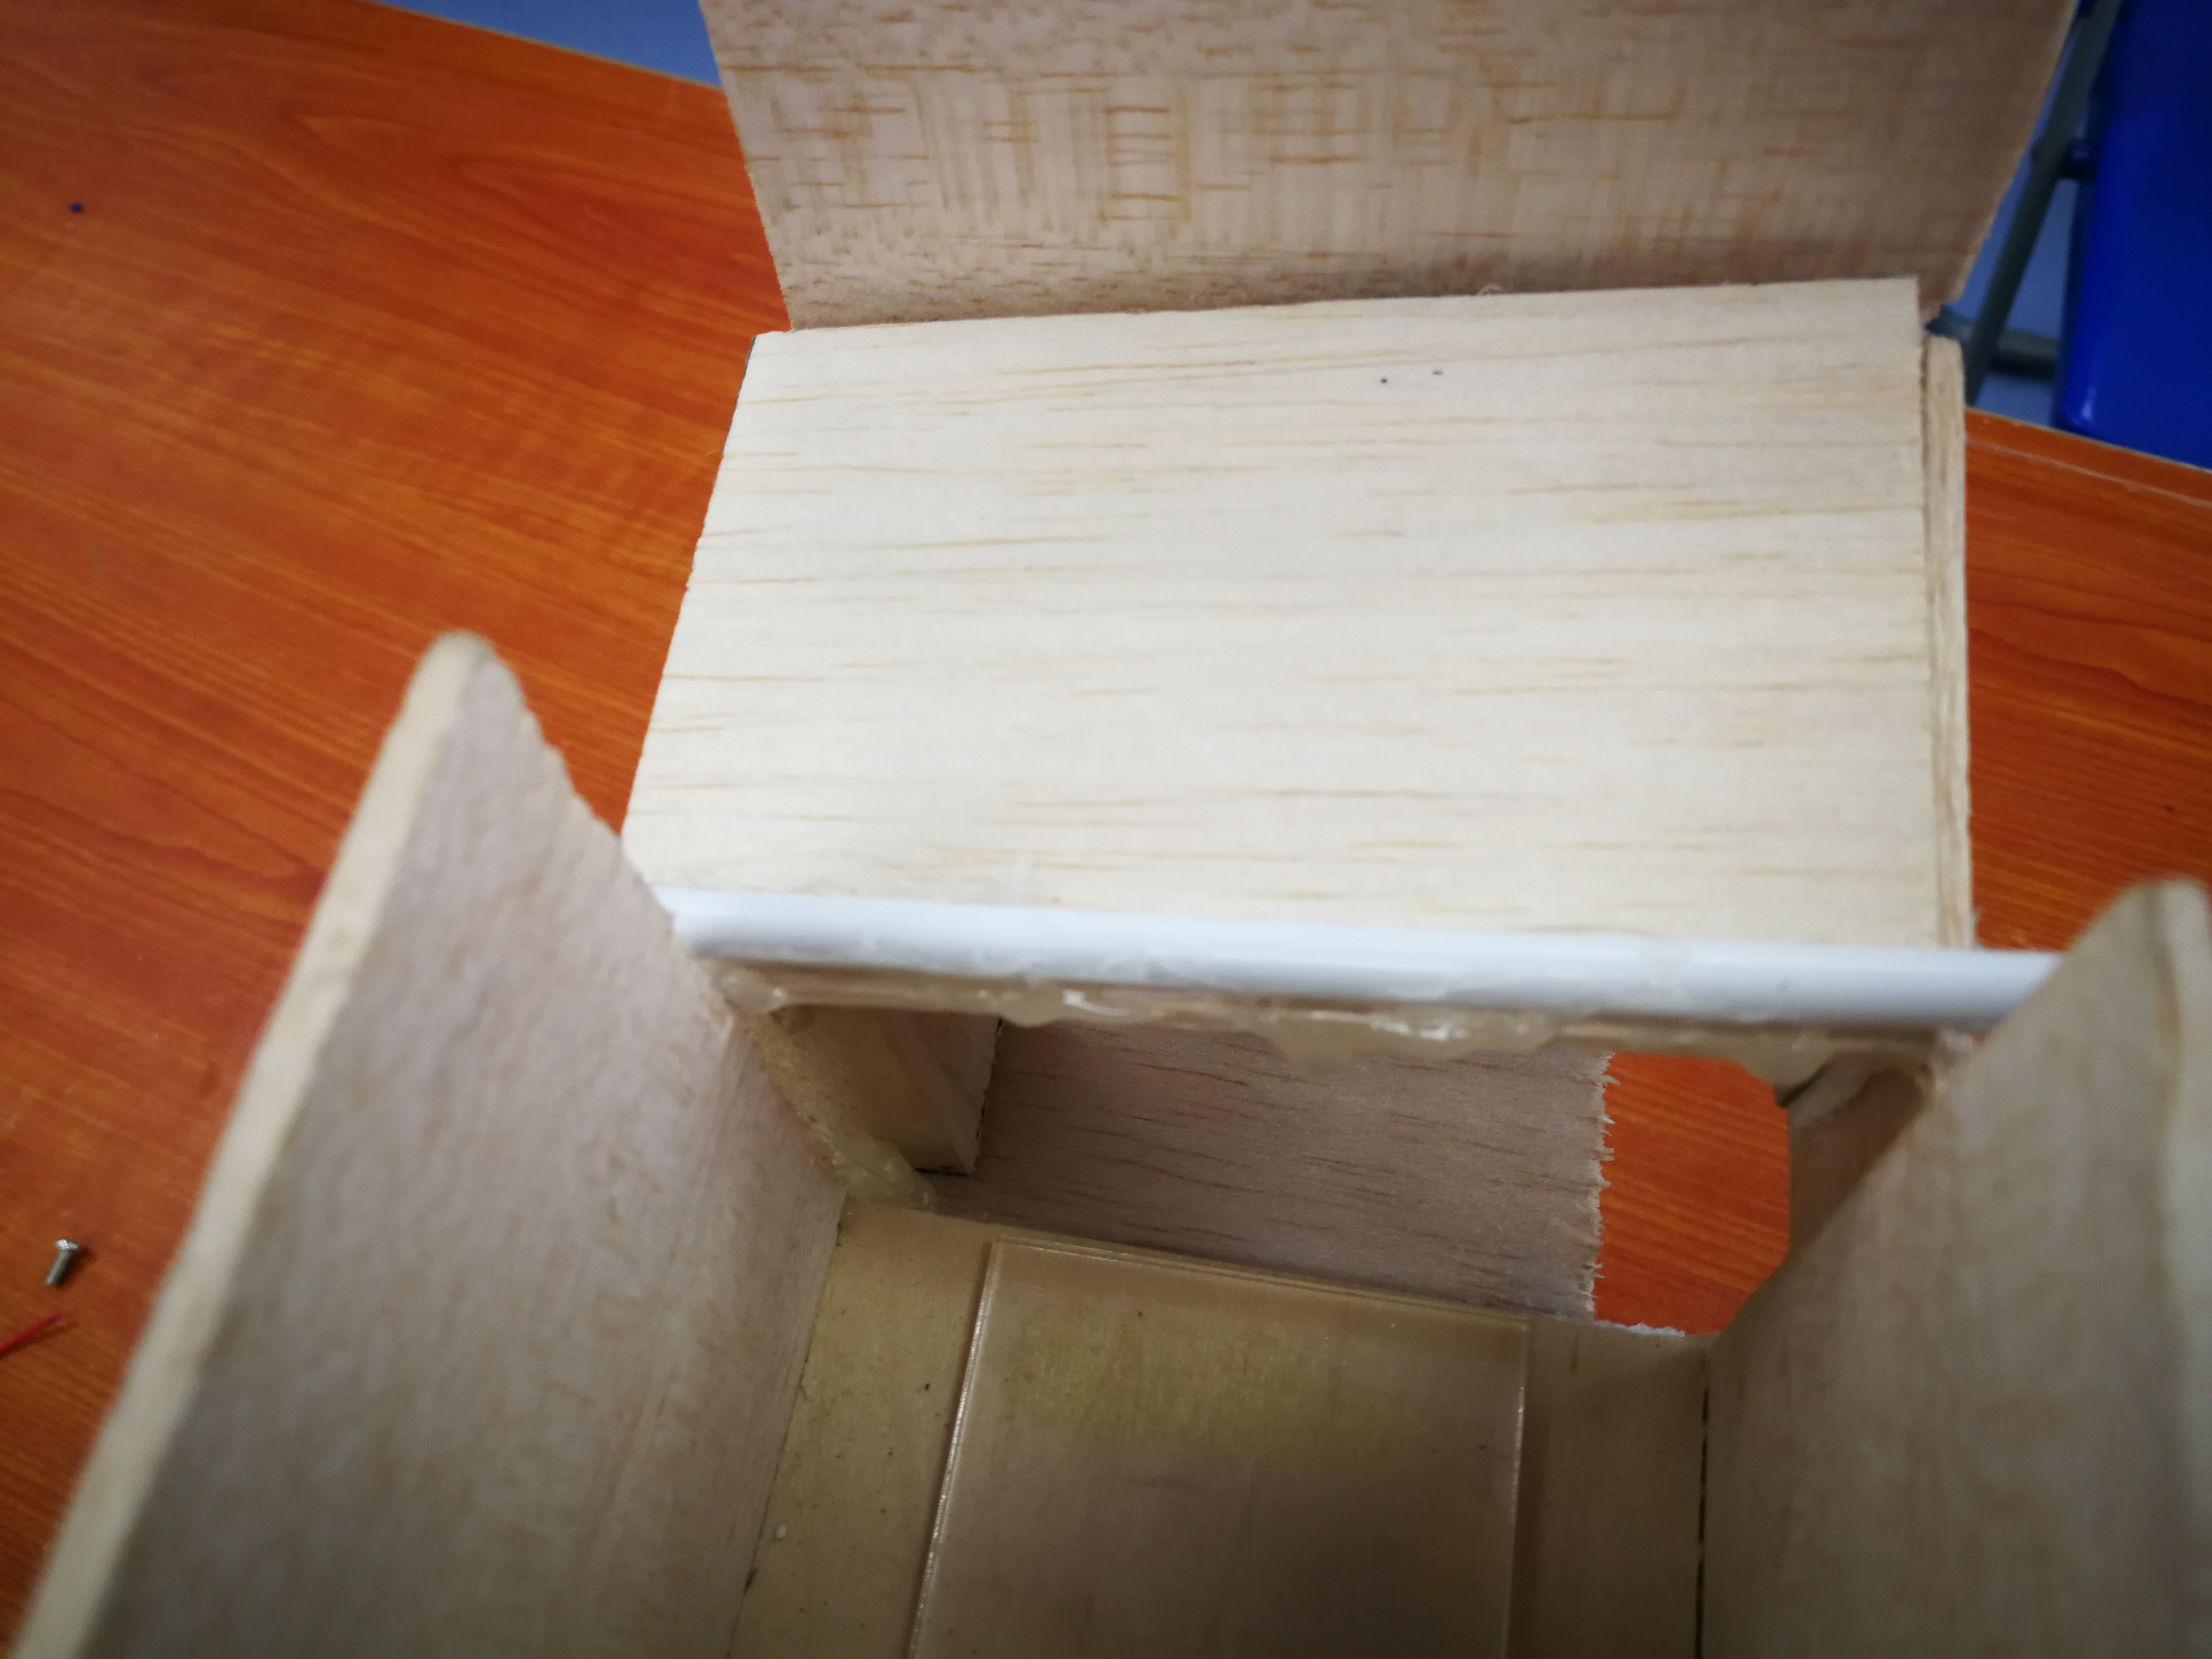
\includegraphics[width=0.5\linewidth]{sti}
\caption{Ramp with a stick.}
\end{figure}

\begin{figure}[H]
\centering
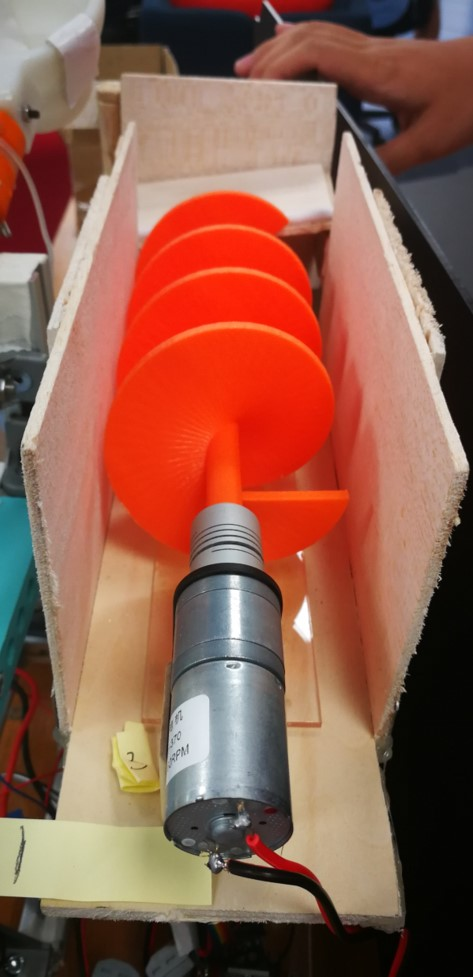
\includegraphics[width=0.4\linewidth]{Screw2}
\caption{Automatic reloading system.}
\end{figure}

\subsubsection*{Shooting System}
The support for the trebuchet arm was made from four alumium beams. Two beams were fixed parallel to the base and the other two beams were attached on top the horizontal beams vertically upwards.  At the top portion, a pillow block that contains bearings and a rod were attached between the vertical beams. This pillow block was attached to 1/3 of the length of trebuchet arm. The bearing and shaft allowed the trebuchet arm to rotate up and down. To prevent the trebuchet arm to rotate left and right, 3 nuts on each side of the center of the bearing were tighten to the shaft.
\begin{figure}[H]
\centering
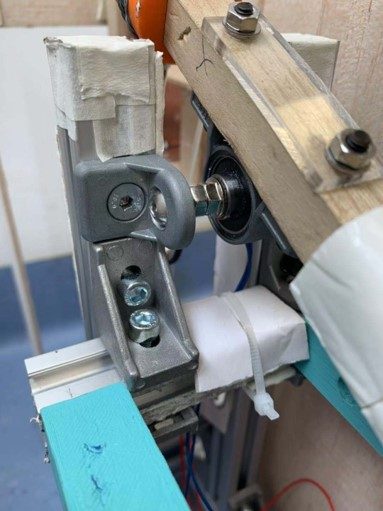
\includegraphics[width=0.3\linewidth]{shaft}
\end{figure}

 To provide the shooting system with the necessary power, a spring was attached to the end of the trebuchet arm.  The spring was folded in half in such a way the end tips of the spring were fasten by screws to the bottom base of the vehicle and the bended portion was attached to the end tip of the trebuchet arm. Here, we use a curve metal plate to achieve the holding while reducing the deformation of the spring (compared with making the spring focus on one sharp part of the beam end).
 \begin{figure}[H]
\centering
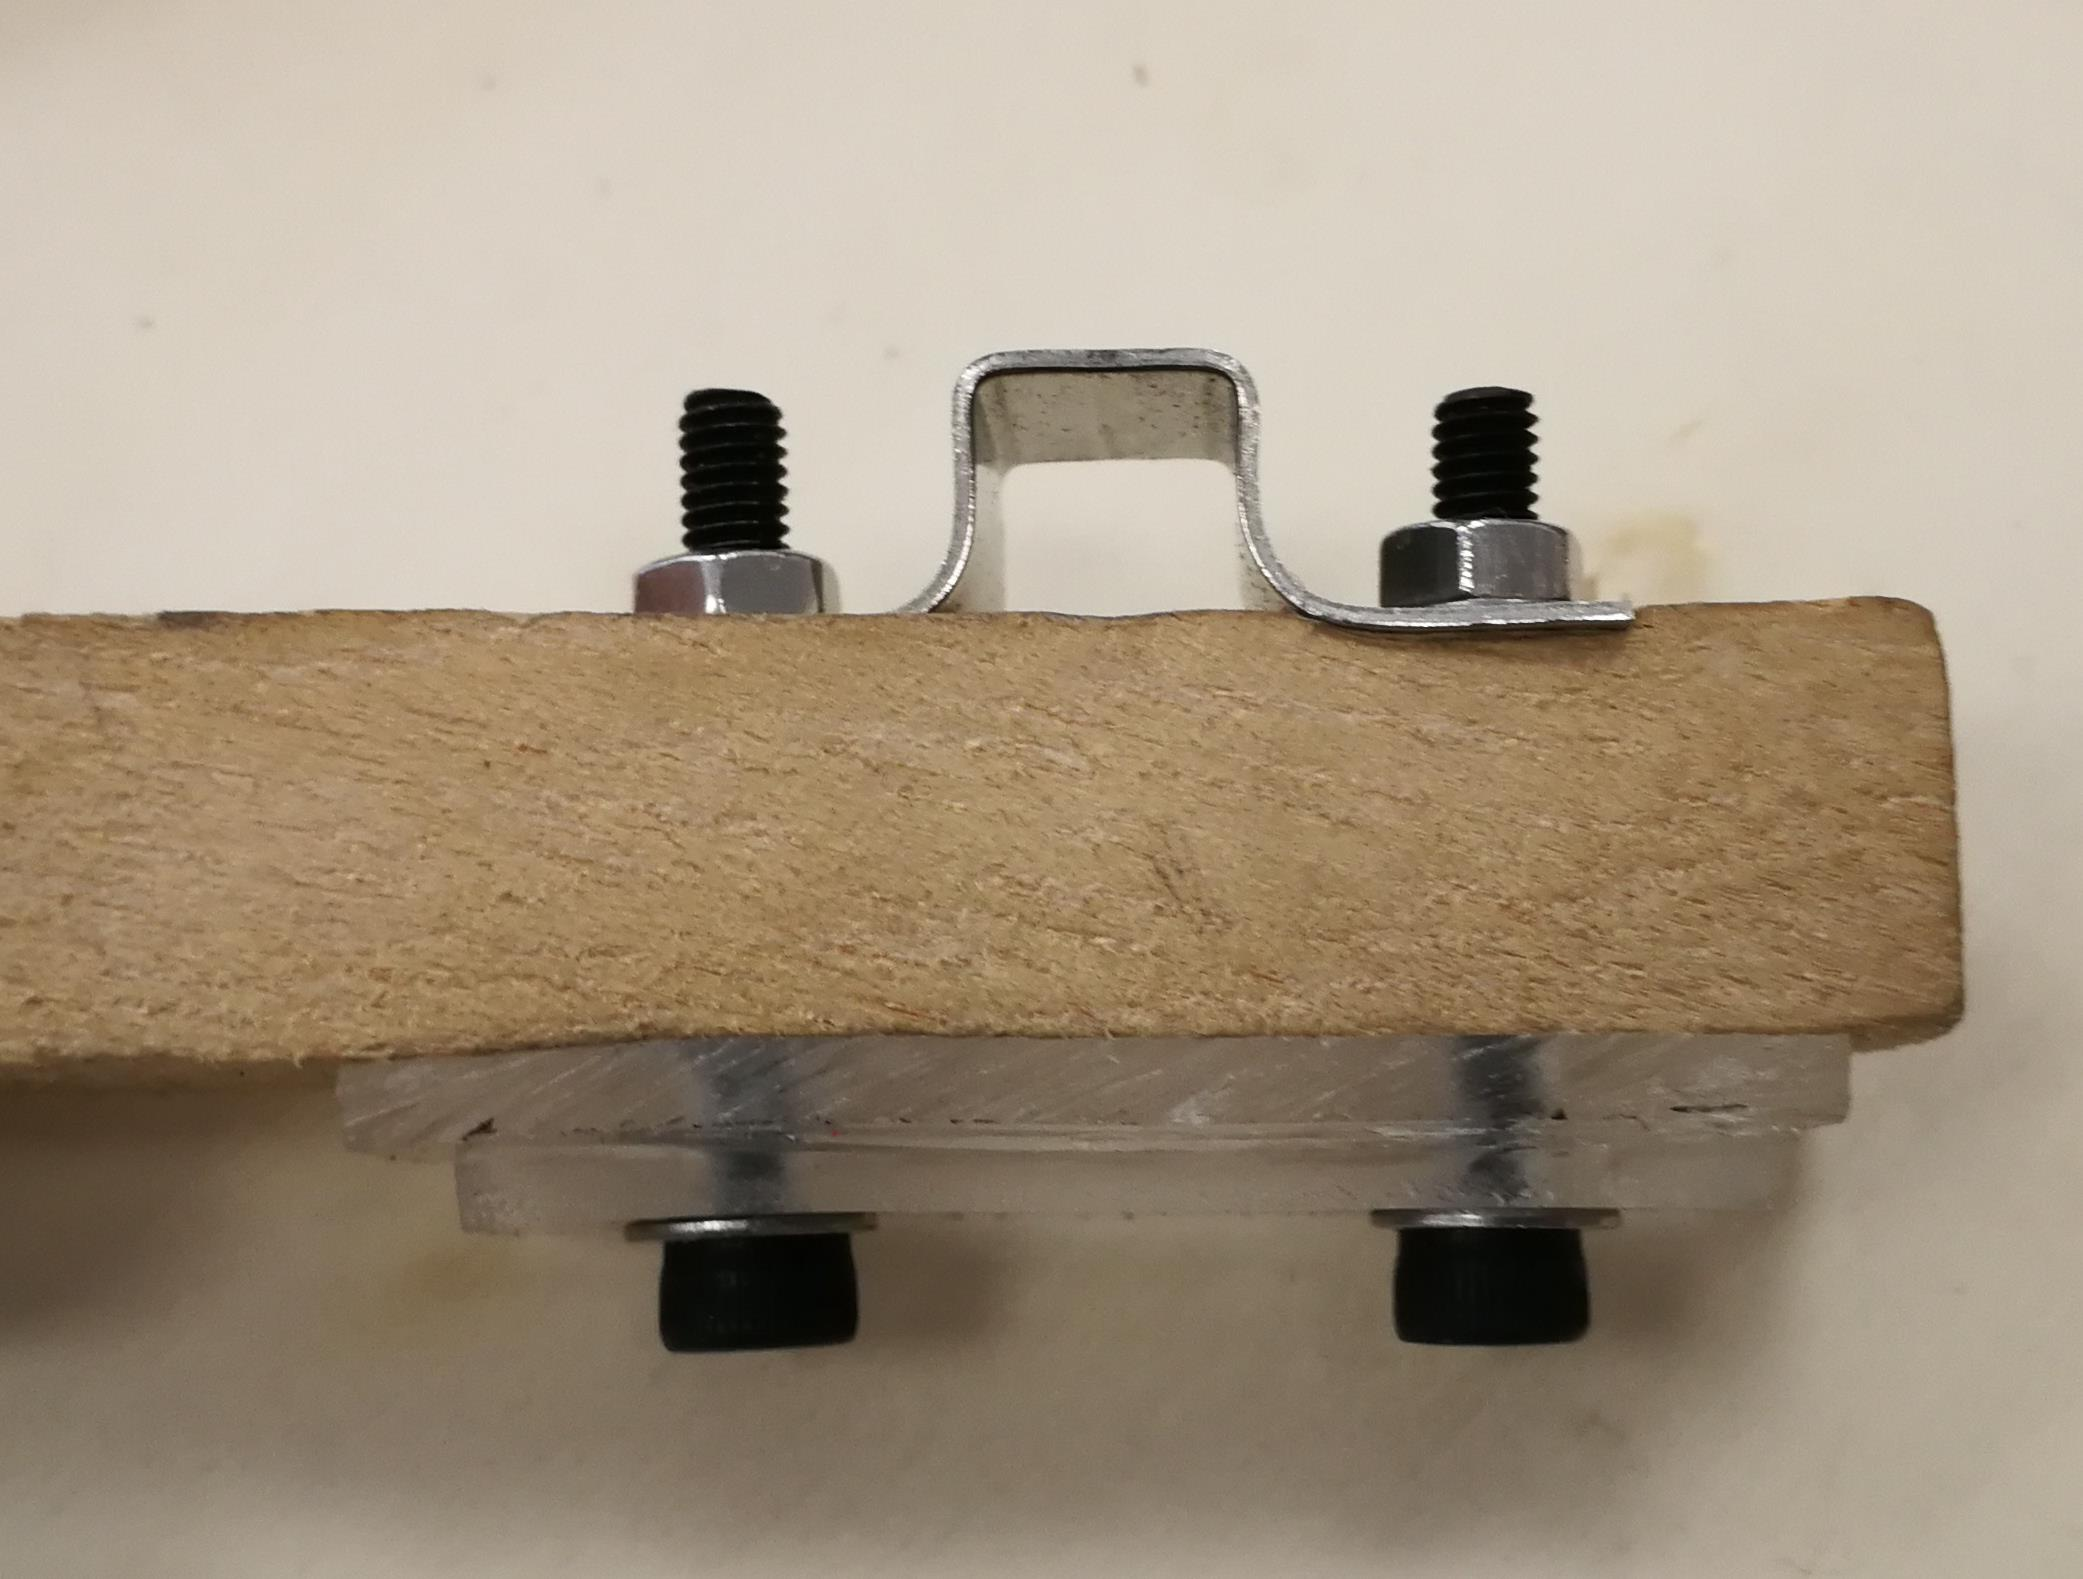
\includegraphics[width=0.4\linewidth]{21}
\end{figure}

We chose wood as the beam for the throwing part, with the cross-sectional area of the beam as $15mm\times 15mm$ so that it fits well to our designed basket. At the top of the beam, we drilled two holes for fixing a stand that connects to the electromagnet and pulling string. The function of this orange stand is that it links the string to the rod in the minimal pressure method, thus the deformation of the wooden rod is minimized.
\begin{figure}[H]
\centering
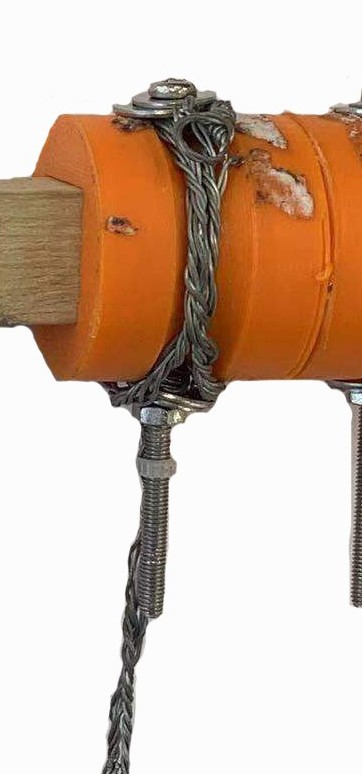
\includegraphics[width=0.14\linewidth]{711}
\caption{Feature of the string stand.}
\end{figure}

\begin{figure}[H]
\centering
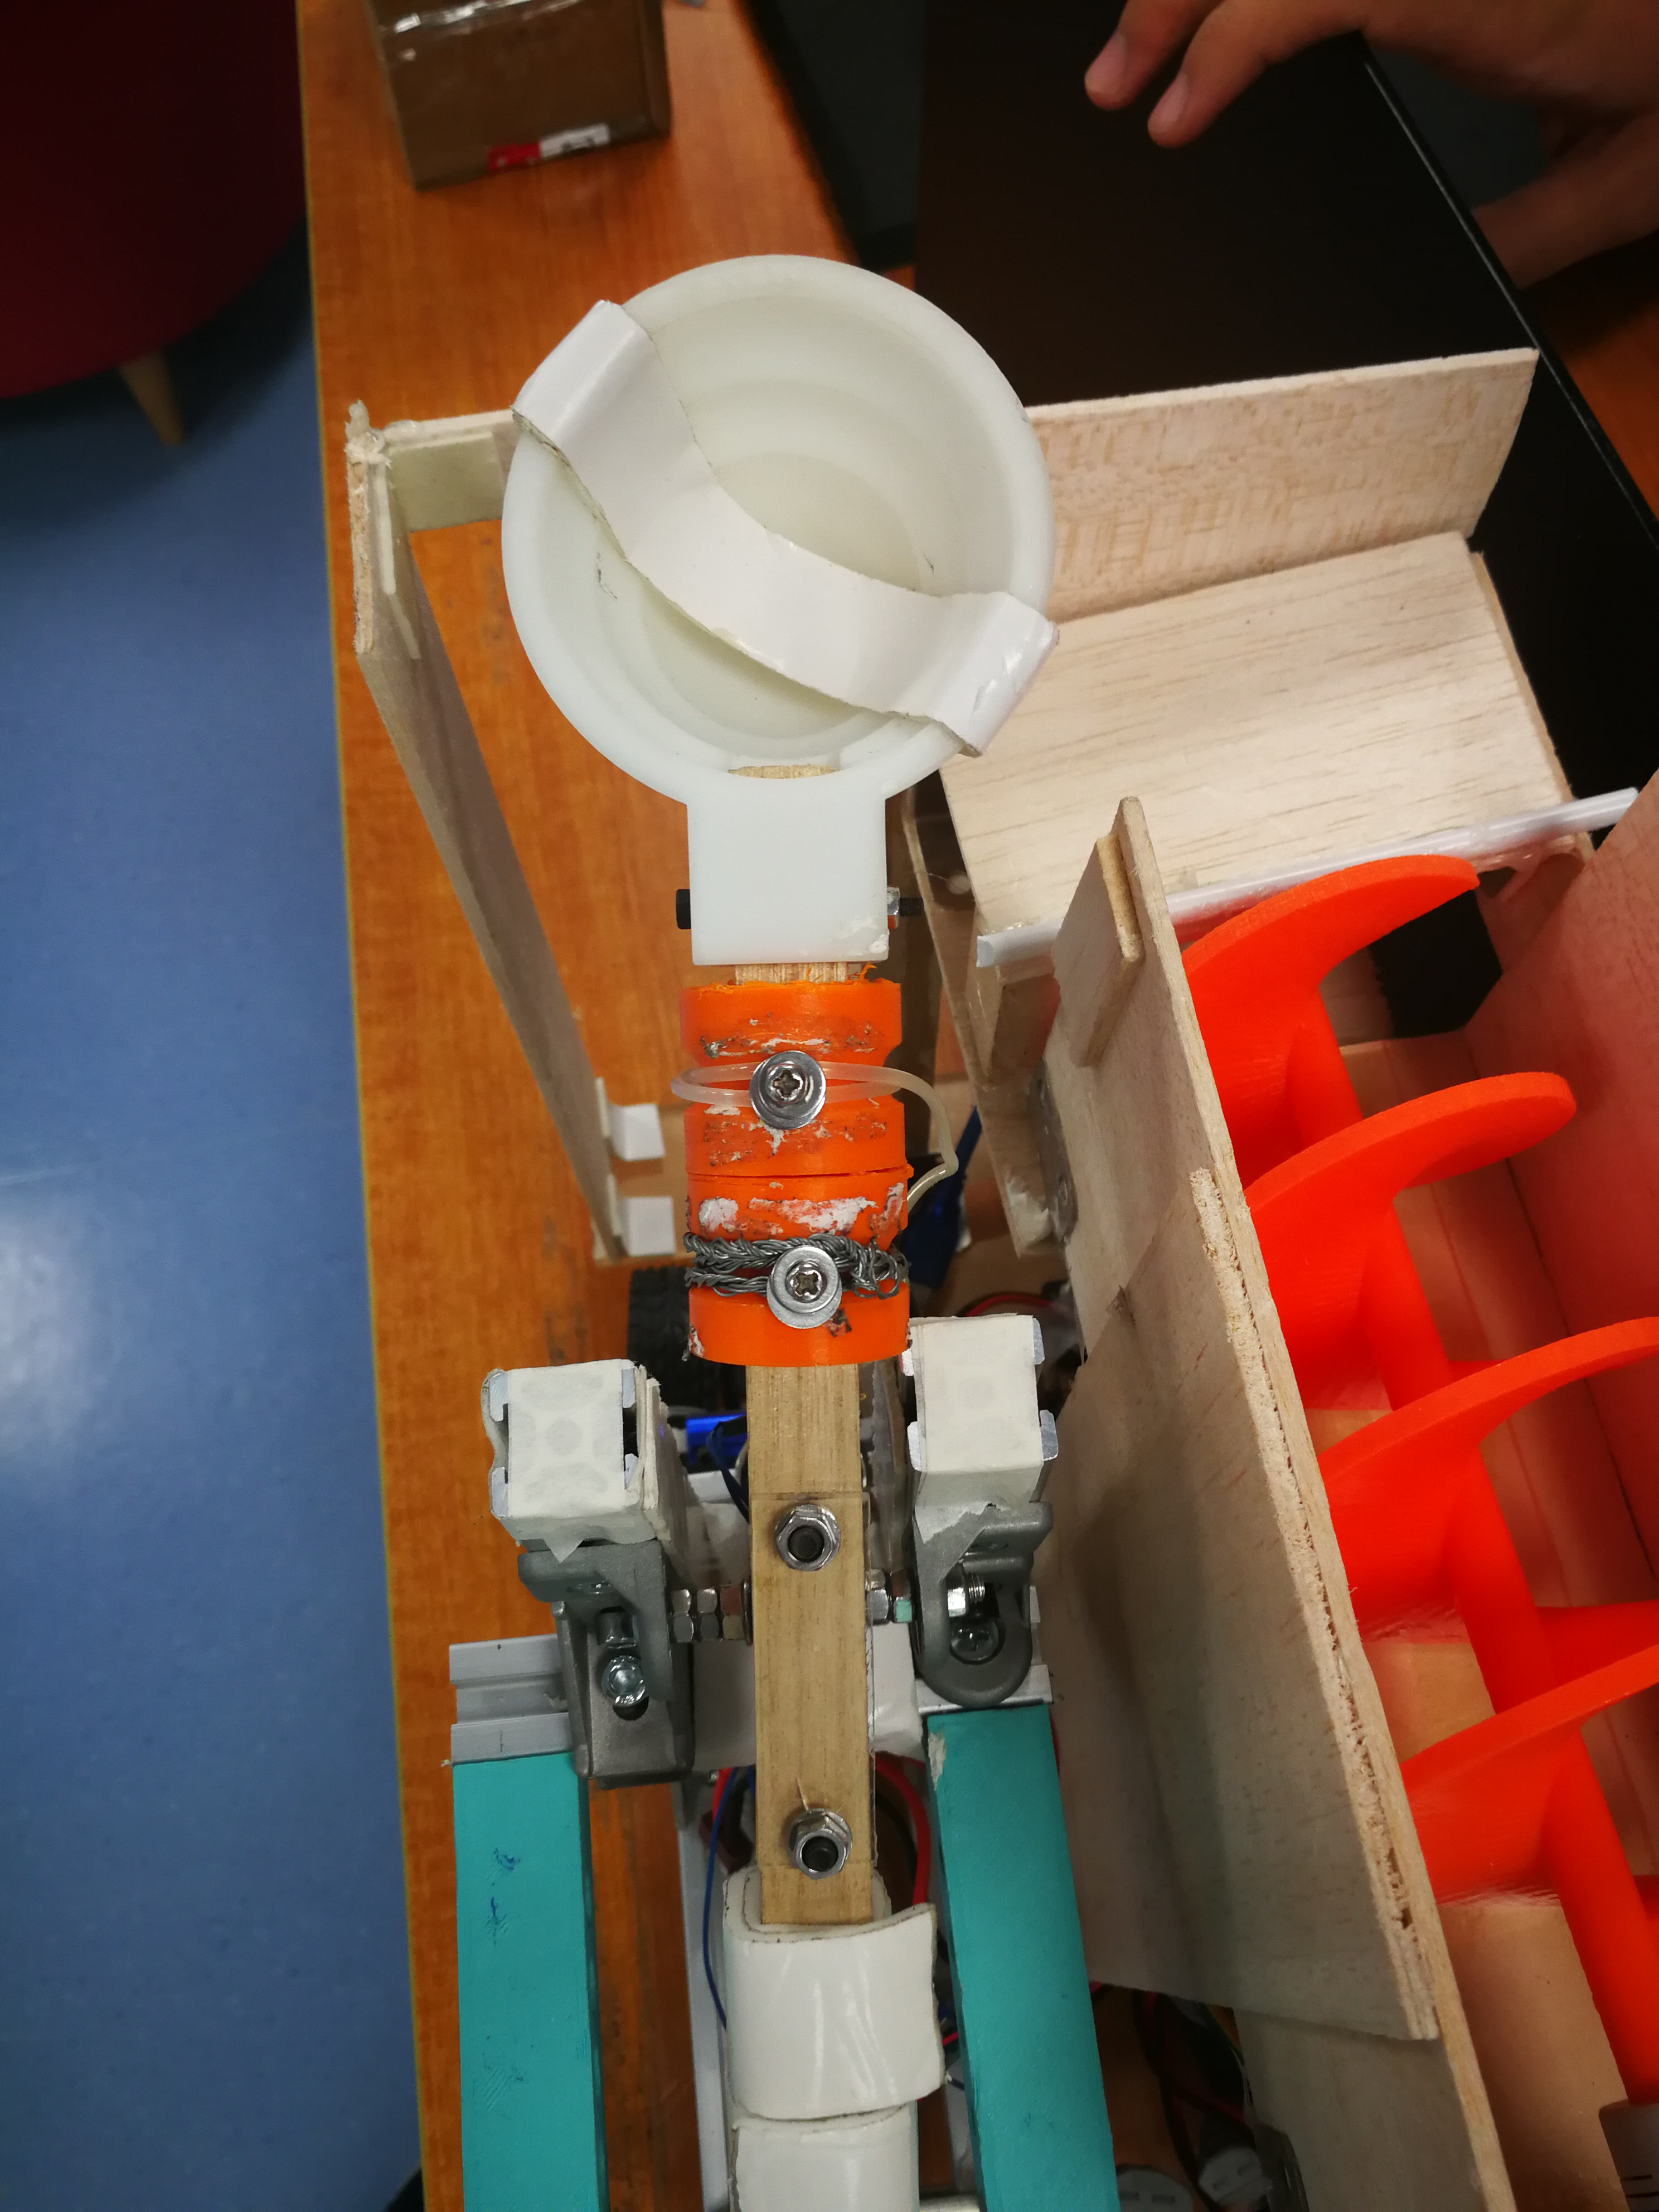
\includegraphics[width=0.4\linewidth]{ass}
\caption{Attachment of the rod to the holder.}
\end{figure}





   A DC motor was attached by angle iron plates between the vertical beams, near the base of the vehicle. This motor rotates a shaft containing fishing wire string that is also connected to the arm of the trebuchet by washers and screws. The hold and release system are compromised by two magnets.  One magnet is placed stationary above the motor, the other magnet contains a screw on the non-magnetic side that enables metal wire that is wrapped around the arm of the trebuchet and the head of the screw to hold the second magnet in tension.  Above the stationary magnet, two angle iron plates were glued to the sides of vertical beams to restrict movement of the second magnet.  
\begin{figure}[H]
\centering
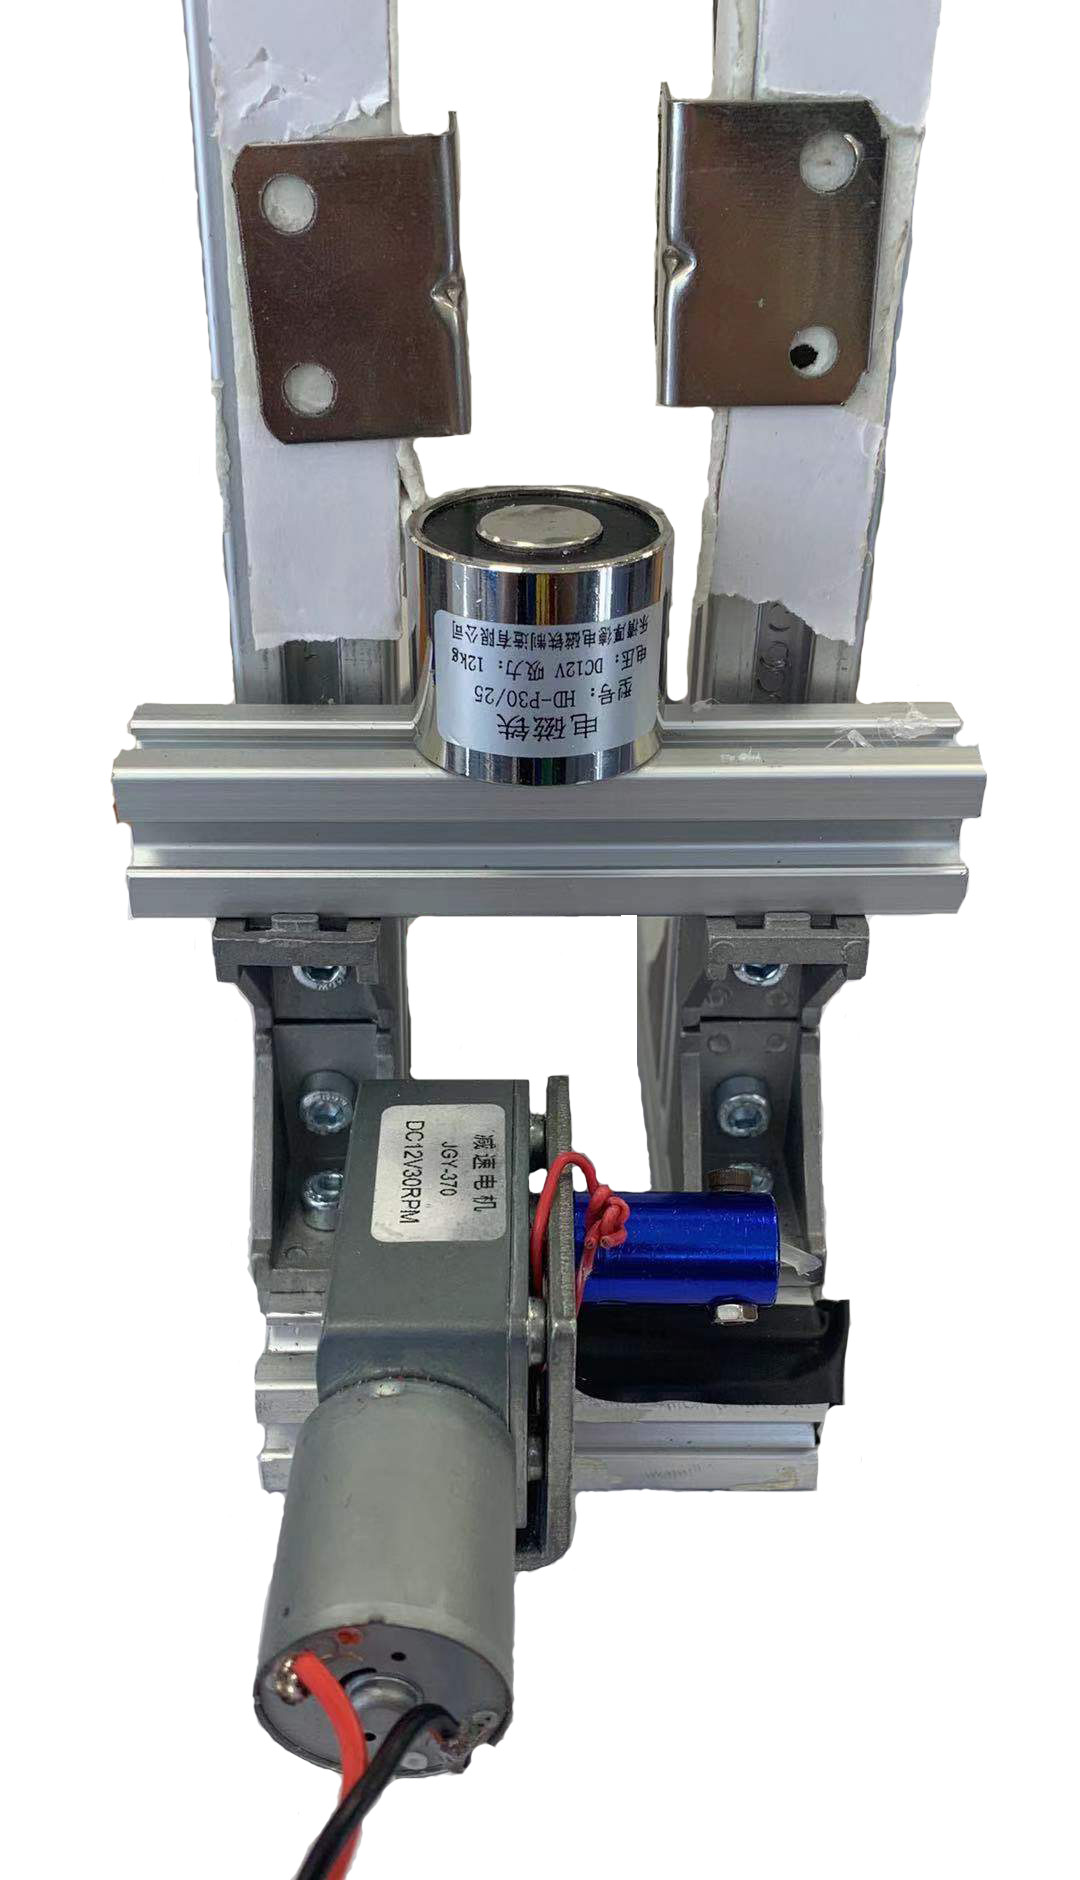
\includegraphics[width=0.35\linewidth]{3}
\end{figure}   

   To control the angle of the launch, two 3-D printed beams with four, 8 mm diameter holes were attached perpendicularly to the vertically beam. An eight-diameter rod, placed inside certain holes, mechanically controls the launch angle of the system.  Therefore, this composites the shooting system.
\begin{figure}[H]
\centering
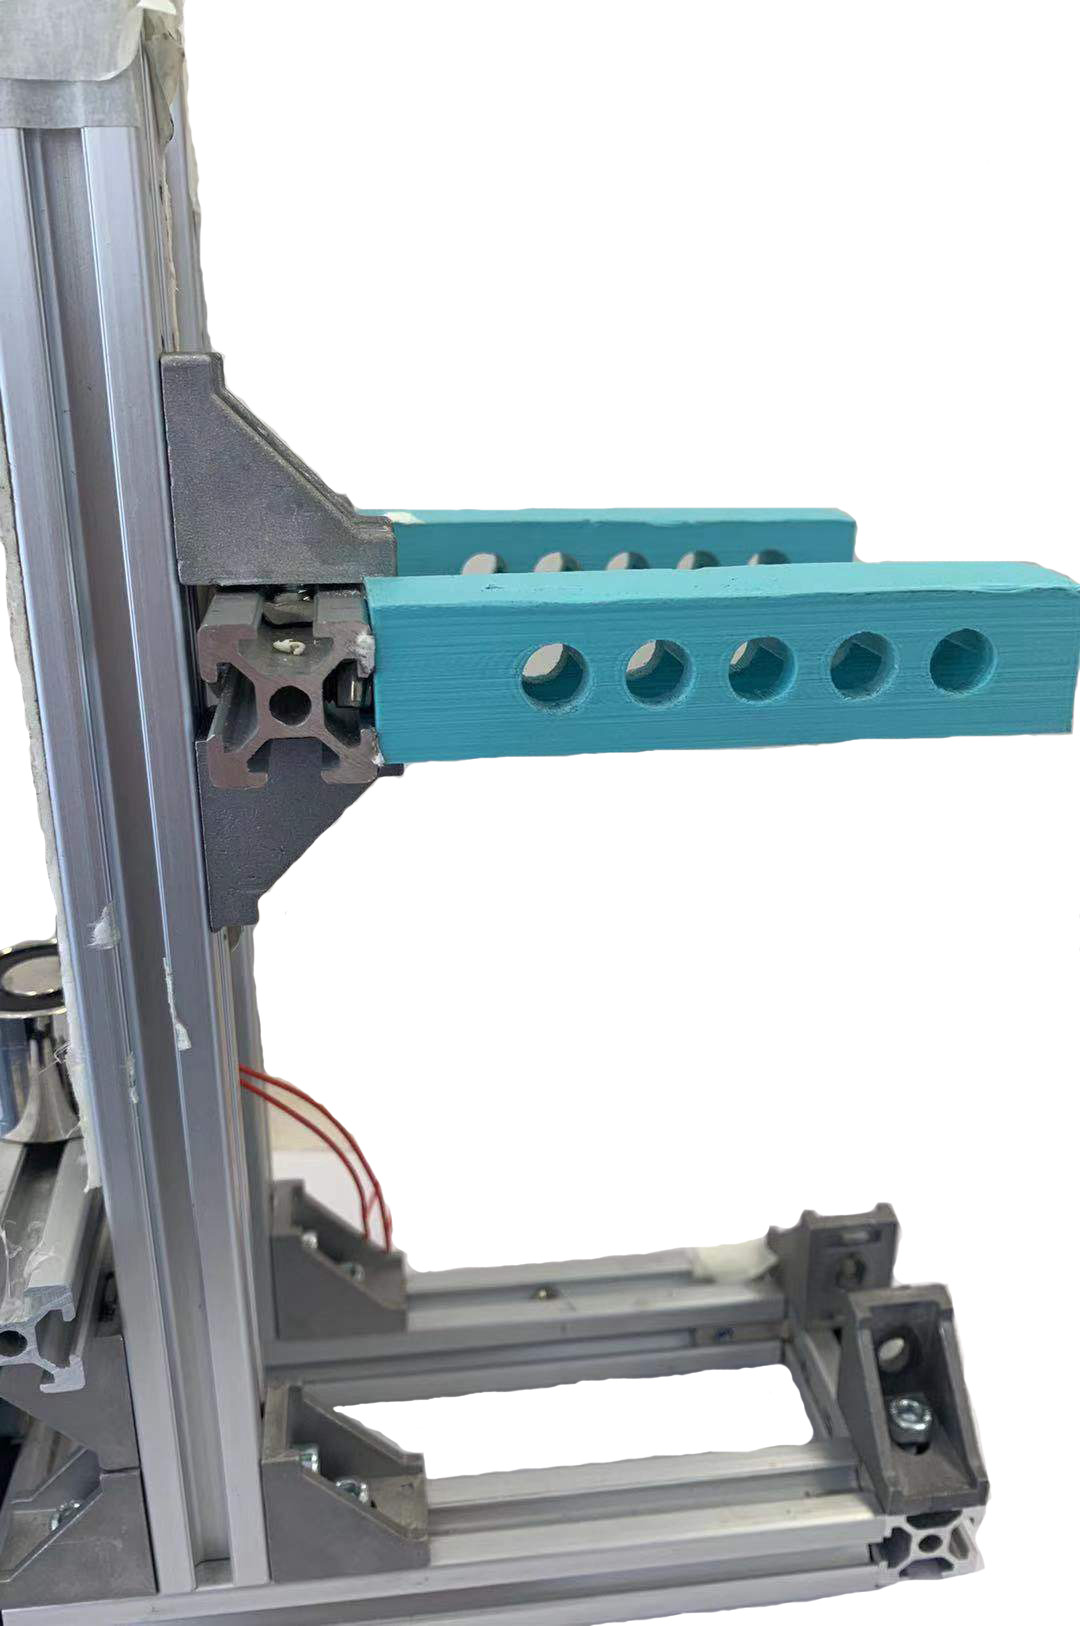
\includegraphics[width=0.35\linewidth]{6}
\caption{Attachment of the haft holder}
\end{figure}

\begin{figure}[H]
\centering
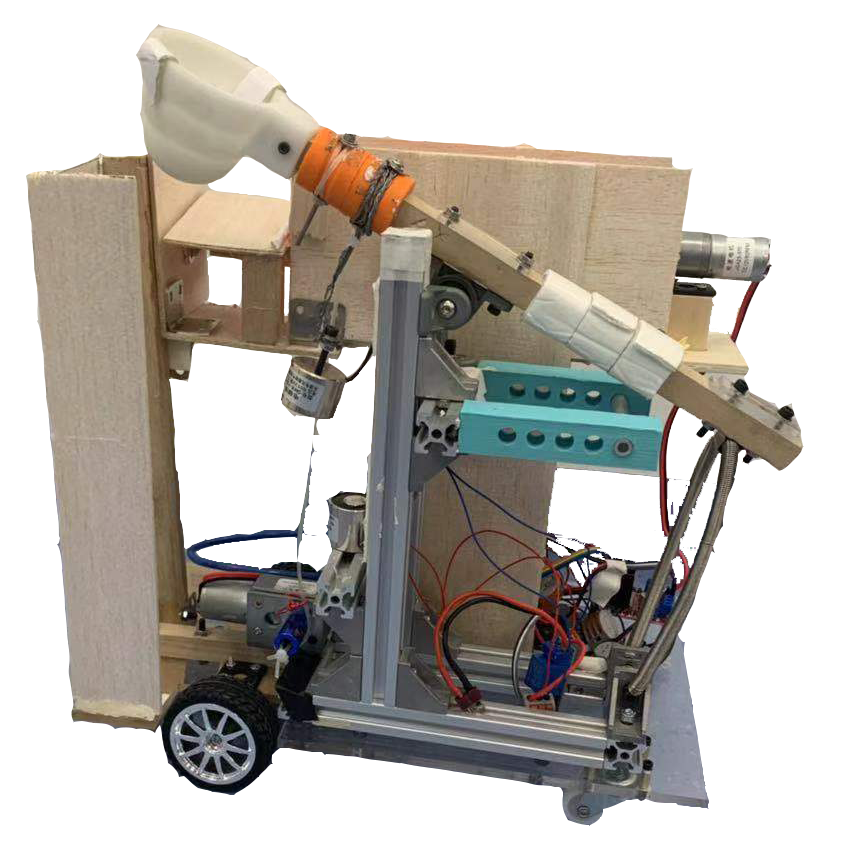
\includegraphics[width=0.4\linewidth]{Car1}
\caption{The overall structure of the car.}
\end{figure}

\subsubsection*{Remote Control}
We design our remote control to accomplish the following functions:
\begin{itemize}
\item Right: Start reloading.
\item Left: Reverse reloading process.
\item Up: Loose the string.
\item Down: Tighten the sring
\item L3: Fix the bar.
\item R3: Loose the bar.
\item L2: Stop reloading.
\item R2: Stop the car.
\item Triangle: Go straight.
\item Circle: Turn right.
\item Cross: Go back.
\item Square: Turn left.
\end{itemize}

The circuit diagram for controlling the driving wheels and the reloading structure is shown below. We use two L298N borads to operate on the four motors. The 12V power input is from the 11.7V battery.

\begin{figure}[H]
\centering
\subfigure{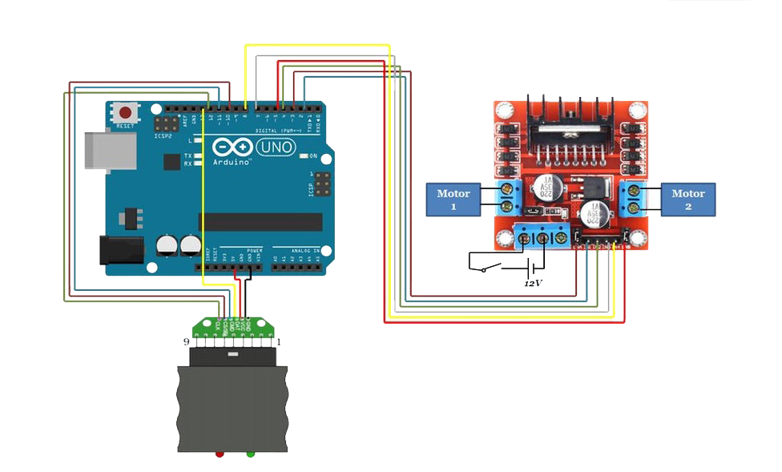
\includegraphics[width=0.7\linewidth]{circuit}}
\caption{The circuit design for the remote control system.}
\end{figure}

For controlling the magnet, we use electric relay to achieve the function of controlling the circuit that links the magnet to the power supply. The PS2 joystick controls the electric relay through the Arduino board. In order to accommodate these pins, we changed from UNO board to MEGA 2560 board, with enough pin holes for us to accomplish this.


\subsection{Production}
\begin{figure}[H]
\centering
\subfigure{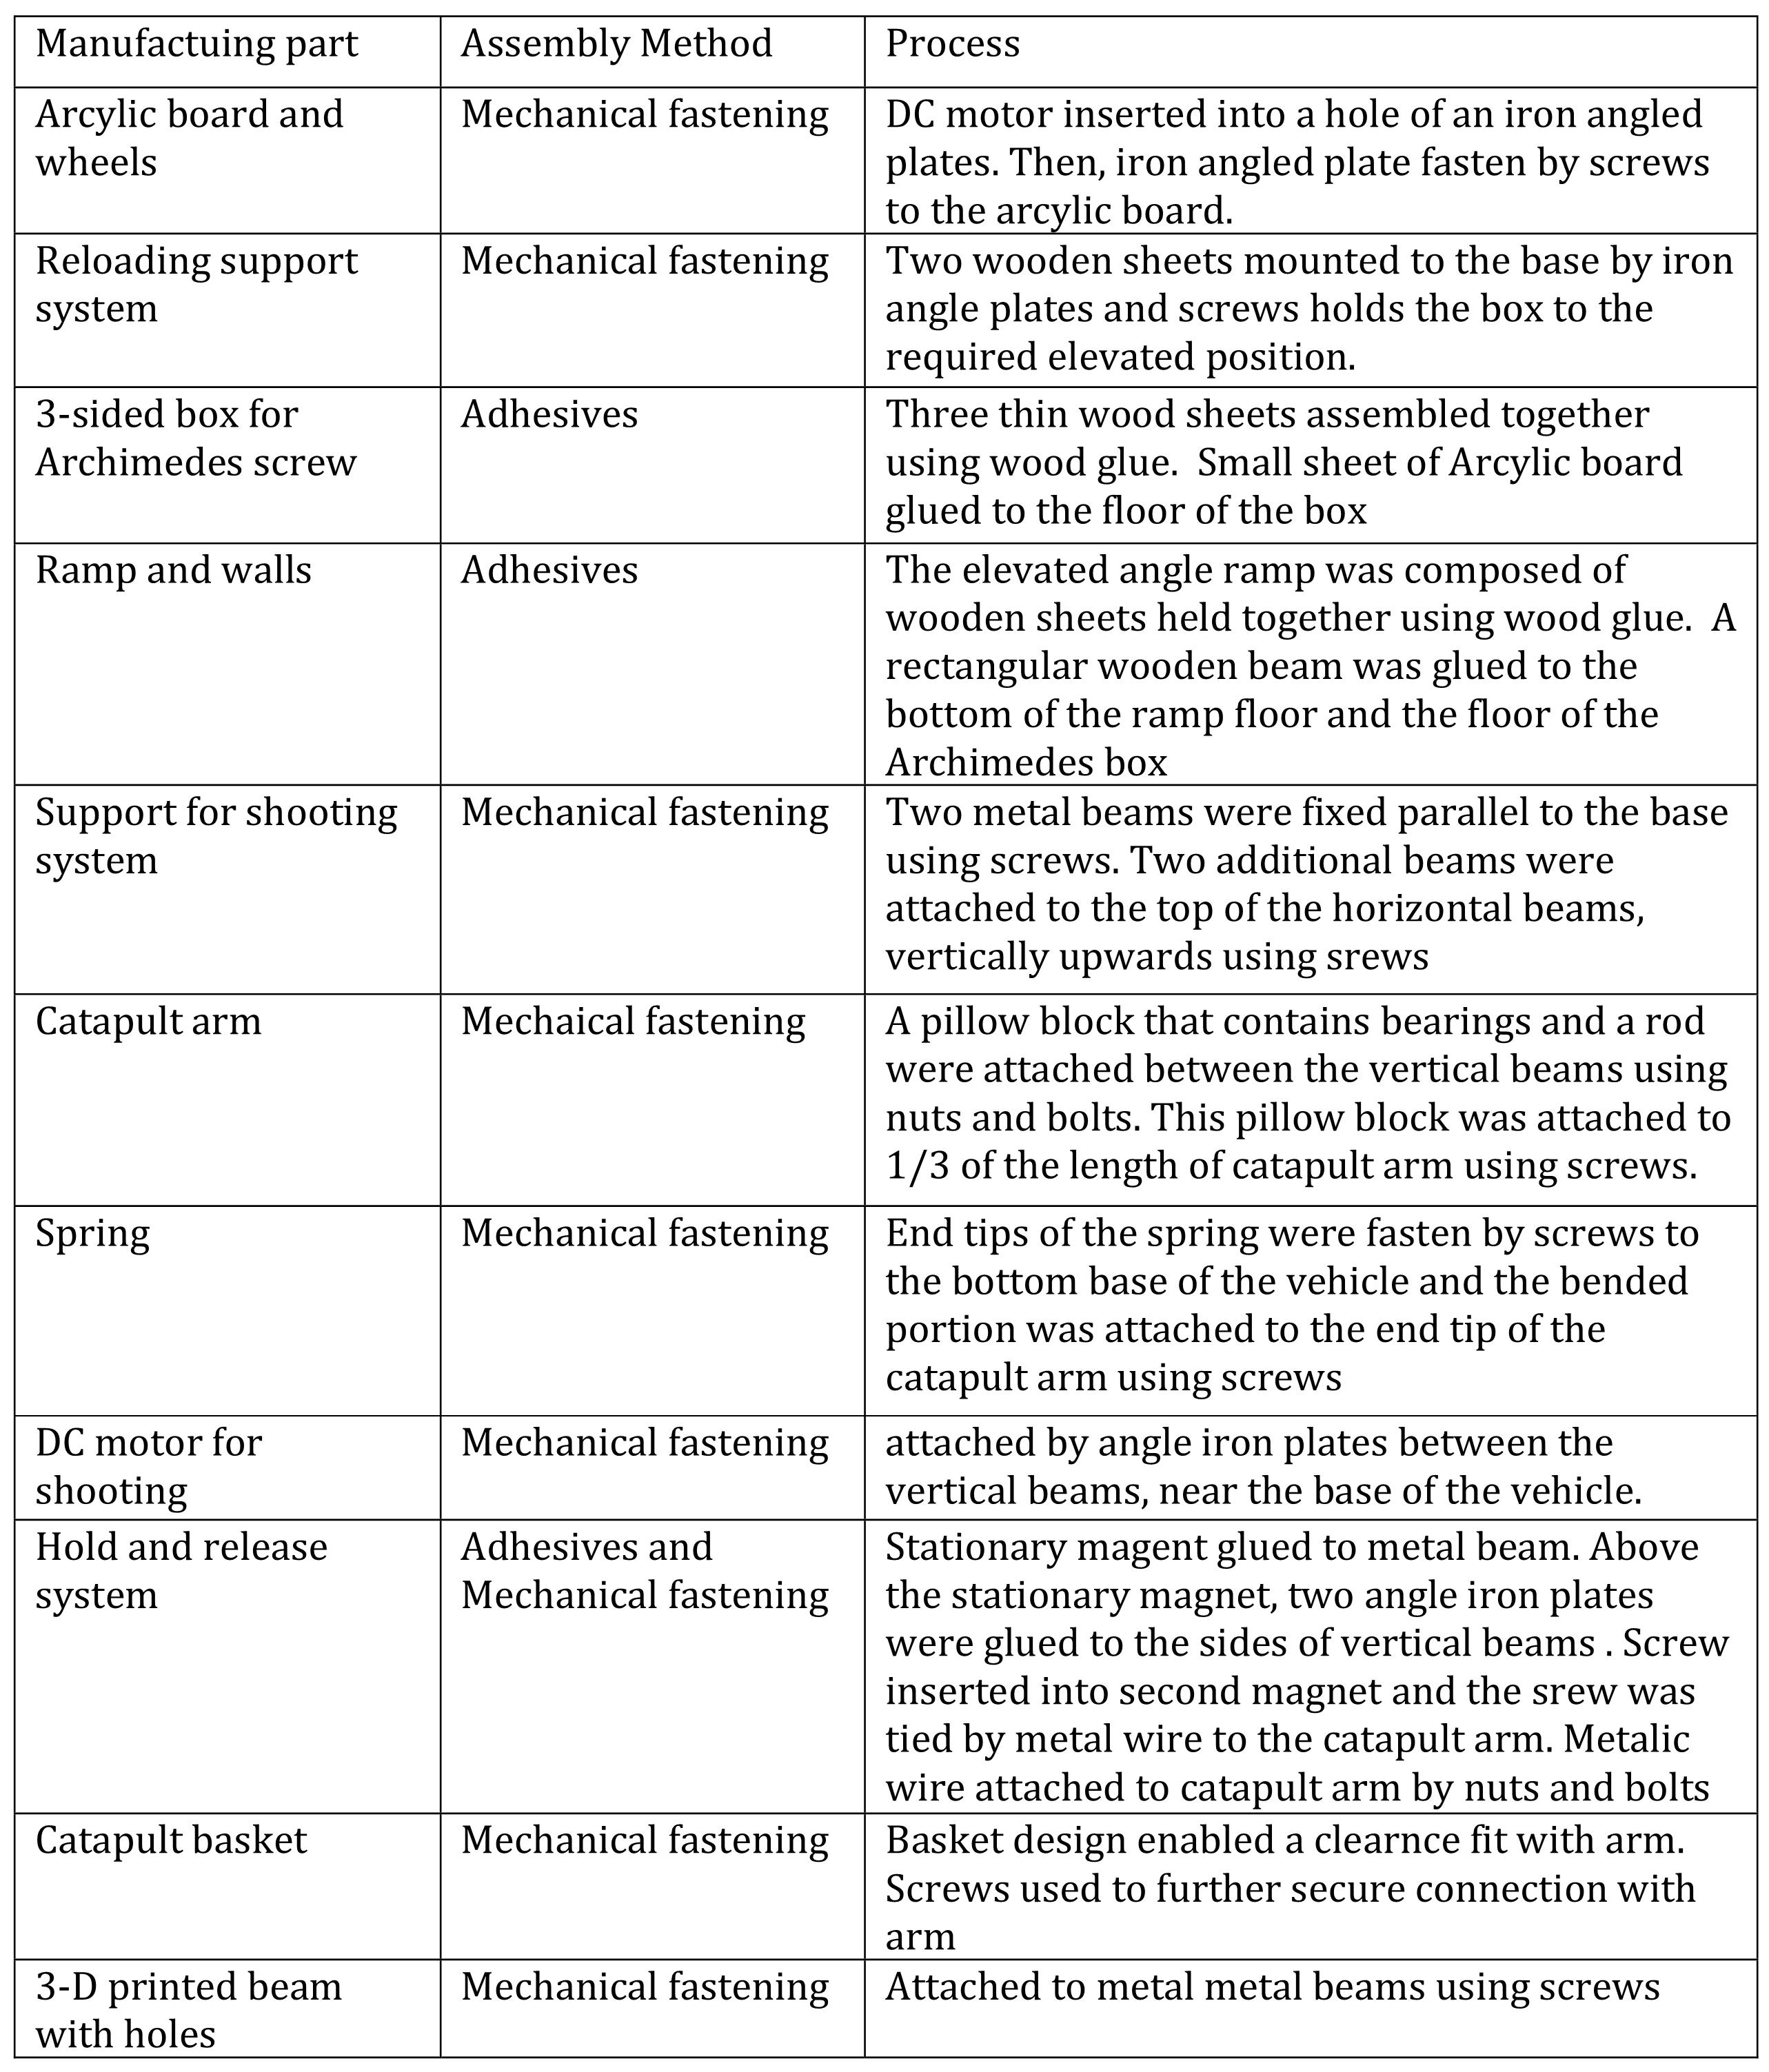
\includegraphics[width=1\linewidth]{table}}
\end{figure}




\section{Cost}
\subsection{Prototype}
\begin{table}[H]
\centering
% Table generated by Excel2LaTeX from sheet 'Separate'
% Table generated by Excel2LaTeX from sheet 'Separate'
\begin{tabular}{|c|c|c|c|}
\hline
\multicolumn{ 2}{|c|}{Item} & \multicolumn{ 2}{|c|}{Price (RMB)} \\
\hline
\multicolumn{ 2}{|c|}{Bearing stand} & \multicolumn{ 2}{|c|}{7.2} \\

\multicolumn{ 2}{|c|}{{\it Electronic Parts (Wires, connector, relay, etc.)}} & \multicolumn{ 2}{|c|}{20.6} \\

\multicolumn{ 2}{|c|}{Tennis balls} & \multicolumn{ 2}{|c|}{8.9} \\

\multicolumn{ 2}{|c|}{Shaft} & \multicolumn{ 2}{|c|}{45} \\

\multicolumn{ 2}{|c|}{12V JGY370 DC motor with stand and links} & \multicolumn{ 2}{|c|}{36.6} \\

\multicolumn{ 2}{|c|}{Hinges} & \multicolumn{ 2}{|c|}{0.88} \\

\multicolumn{ 2}{|c|}{Bowls} & \multicolumn{ 2}{|c|}{16} \\

\multicolumn{ 2}{|c|}{Springs} & \multicolumn{ 2}{|c|}{32} \\

\multicolumn{ 2}{|c|}{Woodboard} & \multicolumn{ 2}{|c|}{34} \\

\multicolumn{ 2}{|c|}{T-shape wires} & \multicolumn{ 2}{|c|}{25.51} \\

\multicolumn{ 2}{|c|}{All-direction wheels (x 10)} & \multicolumn{ 2}{|c|}{8.9} \\

\multicolumn{ 2}{|c|}{502 (Deli)} & \multicolumn{ 2}{|c|}{9.6} \\

\multicolumn{ 2}{|c|}{Woodboard+bar} & \multicolumn{ 2}{|c|}{29.54} \\

\multicolumn{ 2}{|c|}{Acrylic board *2 (For bottom)} & \multicolumn{ 2}{|c|}{60} \\

\multicolumn{ 2}{|c|}{3D Printing module} & \multicolumn{ 2}{|c|}{13} \\

\multicolumn{ 2}{|c|}{Door lock} & \multicolumn{ 2}{|c|}{15.2} \\

\multicolumn{ 2}{|c|}{Motors} & \multicolumn{ 2}{|c|}{72.55} \\

\multicolumn{ 2}{|c|}{Line-direction moving screw \& bar} & \multicolumn{ 2}{|c|}{34.7} \\

\multicolumn{ 2}{|c|}{6mm/4mm to 8mm connection} & \multicolumn{ 2}{|c|}{14.22} \\

\multicolumn{ 2}{|c|}{2020 Aluminum Extrusion} & \multicolumn{ 2}{|c|}{98} \\

\multicolumn{ 2}{|c|}{Electric Magnet} & \multicolumn{ 2}{|c|}{53} \\

\multicolumn{ 2}{|c|}{Arduino Mega} & \multicolumn{ 2}{|c|}{17} \\

\multicolumn{ 2}{|c|}{11.7V Battery} & \multicolumn{ 2}{|c|}{80} \\

\multicolumn{ 2}{|c|}{Screw Rod} & \multicolumn{ 2}{|c|}{24.8} \\
\hline
\multicolumn{ 2}{|c|}{Total} & \multicolumn{ 2}{|c|}{757.2} \\
\hline
\end{tabular}  


\end{table}

\subsection{Production}
During real production, the costing can be expressed using he formula below:
$$Cost/Product=C_m+\frac{C_{oh}}{\dot{n}}+\frac{C_{tool}}{N_t}+\frac{C_{equ}}{N}+C_e+C_i$$
where:
\begin{enumerate}
\item $C_m$ is the cost of material including consumables.
\item $C_{oh}$ is the cost of overhead including labor, administration, etc.
\item $N$ is the quantity of production.
\item $C_{tool}$ is the cost of tools.
\item $N_t$ is the number of products which each tool set can produce in fixed time
\item $C_{equ}$ is the cost of equipments that would not get damaged even for a long time.
\item $C_e$ is the cost of energy.
\item $C_i$ is the cost of information.
\end{enumerate}

\section{Discussion}
\subsection{Design}
\subsubsection*{Hold/release system}


Initial design have the lock (Figure 36). It's purpose to control the length of stretching of the spring, so we are able to throw all types of balls, as we have different forces of the spring at different lock positions. The main goal of the lock is to hold and release the basket to shoot. However, there are some problems with this design. It is hard to attach it to the basket. Also, due to limitation of the size of our vehicle, we supposed to use shorter bar if we use this lock. This will limit the power output of the whole system. In addition to these, it is complicated to manufacture. Therefore, we decide to change our design. 


\begin{figure}[H]
\centering
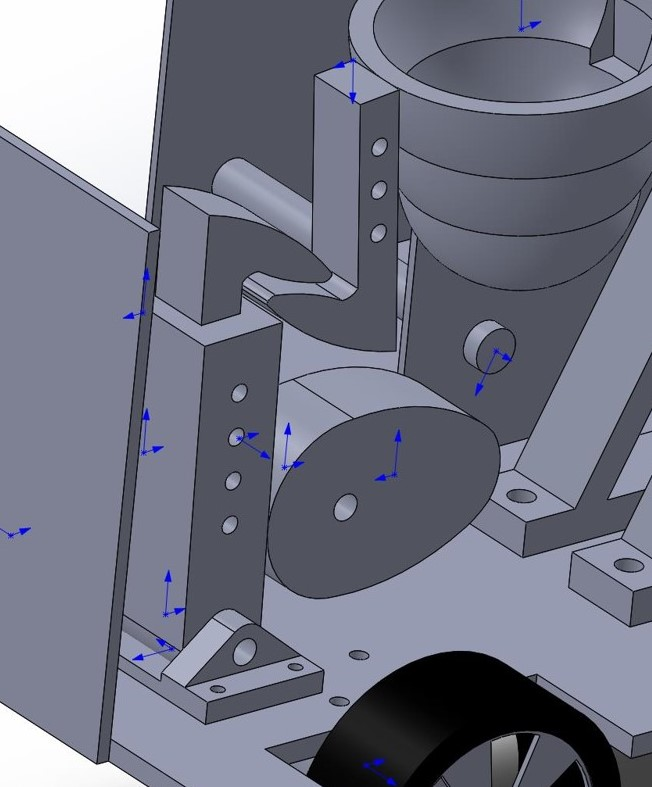
\includegraphics[width=0.3\linewidth]{Lock}
\caption{Initial Hold/Release system design.}
\end{figure}

\par
New design consist of two magnets and two rods with holes along their length (Figure 37). Magnets serve as the holding/realising mechanism. Two rods and a shaft between them limit the rod movement. In this way we control the angle at which our ball will fly off from the basket. Different angles provide different trajectory, so different throw distance. In this way we can achieve different types of balls to fly the same distance. 


\begin{figure}[H]
\centering
\subfigure{\includegraphics[width=0.3\linewidth]{6}}
\subfigure{\includegraphics[width=0.32\linewidth]{233}}
\caption{Final Hold/Release system design}
\end{figure}

\subsubsection*{Center of mass}
Due to unequal mass distribution on our vehicle, center of mass was approximately near the front wheels. This problem cased bad motion of our vehicle. As back wheels are driven wheels, the did not have a good connection with the ground. To solve this issue we located all power sources such as portable charger and batteries on the back of our vehicle. This load changed the center of mass closer to the back wheels, so our robot became more navigable.
\subsection{Manufacturing}
\subsubsection*{Wooden rod}
Main part of our vehicle is the wooden rod (Figure 38). There are 6 components located on it: spring connection(1), thick tape(2), bearing connection(3), hold/release system steel wire connection(4), pulling shark fishing wire connection (5), basket location(6). 

\begin{figure}[H]
\centering
\includegraphics[width=0.7\linewidth]{71}
\caption{Rod}
\end{figure}

During manufacturing process we added hard plastic rigid plates below bolts' hat (1),(3). Their purpose is to take the part of bending stress occurring due to stretching the spring. In this way, we increase the life time of our wooden rod. Thick tape (2) takes the stress during the collision with the bar that set the final angle of the wooden rod.
Special orange cylinders with the through hole and a gap for a wire (4),(5) help to fix wire and prevent them from sliding.  

\subsubsection*{Pulling wire}
For pulling wire we tested several kind of wires and ropes. Due to large normal stress most of them broke either in the middle or near the motor. Materials that we used: fiber rope(2mm), river fishing line wire, fiber rope(6mm),steel wire(0.2mm), copper wire(1mm), shark fishing line wire (Figure 39).


\begin{figure}[H]
\centering
\subfigure{\includegraphics[width=0.25\linewidth]{2}}
\subfigure{\includegraphics[width=0.133\linewidth]{50}}
\subfigure{\includegraphics[width=0.1\linewidth]{51}}
\subfigure{\includegraphics[width=0.108\linewidth]{52}}
\caption{Different types of tested wires}
\end{figure}

\subsubsection*{Hold/release system}
Three problems occurred during the manufacturing of the hold/release system. Firstly, the strength of the wire, that holds the top magnet. It should be able to take high normal stress. In addition to this,it has to be hard deformable, so that it magnet alignment can be achieved after several shots. To solve this problem we connected 8 steel wires (Figure 40). It provides enough strength and does not deform a lot after shooting.

\begin{figure}[H]
\centering
\includegraphics[width=0.2\linewidth]{711}
\caption{Wire for Hold/release system}
\end{figure}

\par 

Secondly, strong connections between top and bottom magnet should be achieved. Initially we wanted to use one magnet and the iron plate (Figure 41) to save money and energy consumption. However, it was almost impossible to manufacture, as not full surface of a plate connects to a magnet. But to provide enough force to hold the stretched spring, plate should be fully attached to a magnet. 
\begin{figure}[H]
\centering
\includegraphics[width=0.4\linewidth]{54}
\caption{Iron plate}
\end{figure}

\par 
Thirdly, magnet alignment should be achieved. After shooting, top magnet can freely move, as it connected with deformable steel wire. So, to limit it's position after pulling the rod down we placed two angle iron plates. As magnet connected to the power source too, we had to leave the space between these angle iron plates(Figure 42). Furthermore, the advantage of using these two magnets is that they create the magnetic field that interact between each other. So at the bottom position they are adjusting their position by themselves.
  
\begin{figure}[H]
\centering
\subfigure{\includegraphics[width=0.24\linewidth]{3}}
\subfigure{\includegraphics[width=0.32\linewidth]{233}}
\caption{Angle Iron plates}
\end{figure}

\subsubsection*{Bearing connection}
To shoot accurate and consistent we had to achieve no movement of the rod besides the rotation of the plane. Also, to shoot far, it is important to avoid as much friction as we can, so there is no additional lose in energy. So there should be enough distance between support metal bars, but the bearing should be tightly connected. Our solution is to use a lot of nuts. They don't have a big diameter, so they will not affect other parts besides bearing. Furthermore, they can tightly clutch the bearing, so it's movement is limited (Figure 43).

\begin{figure}[H]
\centering
\includegraphics[width=0.3\linewidth]{11}
\caption{Bearing connection}
\end{figure}


\subsection{Testing}
To shoot on 2 meters, in our case, we should provide enough length of stretched spring. The best condition during our testing procedure, the length of the stretched  spring is 35(cm). So, we have made an appropriate length of the wire that connects top magnet to the rod. 

\subsection{Reflections \& Recommendations}
During the game day, we found out that after continuous shooting for 10 minutes, the power of the spring decreases with time. So, to be more accurate, it is better to start with balls with higher weight (in our case tennis ball) and keep spring not stretched during the vehicle movement or when it is not needed.
\par 
For material of the reloading system, it is better to use metal or plastic. As rocket balls and the wood has high friction, we can not reload rocket balls with our final structure.
\par 
Locating magnets as much further as possible from the pivot point will save more electric energy.
\section{References}
\begin{enumerate}
\item Basic Arduino PS2X controlling code. \url{https://github.com/madsci1016/Arduino-PS2X/blob/master/PS2X_lib/examples/PS2X_Example/PS2X_Example.ino}
\item 2020 alumium extrusion, \url{https://s.1688.com/kq/-32303230C2C1D0CDB2C4.html}
\end{enumerate}

\section{Acknowledgements}
\par For the project set-up and material purchasing, we would like to thank Prof. Li Mian, TA Zhang Chenzhi \& Chen Jiaxi. Throughout our manufacturing, their suggestions and guidance are very useful. The lectures Prof. Li Mian taught are also very helpful as they form the theoretical basis for our manufacturing.\\

We would like to acknowledge the other students in other groups for their suggestions during the design review, and the lab faculty who also gave us much assistance towards drilling and 3D printing.\\

Finally, each person in our group is grateful for other team members' efforts as our success during the demonstration is the result of our team effort.
\newpage

\section{Appendix}
\subsection*{Codes for this project.}

%%%%%%%%%%%

\begin{lstlisting}[language={C}]
#include <PS2X_lib.h>  //for v1.6
/*****************************
 * set pins connected to PS2 controller:    16//10  //16
 * 
  */
#define PS2_DAT        14     
#define PS2_CMD        15 
#define PS2_SEL        16  
#define PS2_CLK        17 
//Moving Car
int pinI1=6;//I1
int pinI2=7;//I2
int pinI3=8;//I3
int pinI4=9;//I4
//Reloading + pulling
int pinI5=2;
int pinI6=3;
int pinI7=4;
int pinI8=5;
//The electro magnetic (using the electric relay)
int relay=30;   //

/******************************
 * select modes of PS2 controller:
 *   - pressures = analog reading of push-butttons 
 *   - rumble    = motor rumbling
 * uncomment 1 of the lines for each mode selection
 **********************************/
#define pressures   true
//#define pressures   false
#define rumble      true
//#define rumble      false

PS2X ps2x; // create PS2 Controller Class

int error = 0;
byte type = 0;
byte vibrate = 0;

void setup(){
 
  Serial.begin(115200);
  //**************
  delay(300);
  //**************
  pinMode(pinI1,OUTPUT);
  pinMode(pinI2,OUTPUT);
  pinMode(pinI3,OUTPUT);
  pinMode(pinI4,OUTPUT);
  pinMode(pinI5,OUTPUT);
  pinMode(pinI6,OUTPUT);
  pinMode(pinI7,OUTPUT);
  pinMode(pinI8,OUTPUT);
  pinMode(relay,OUTPUT);
  //pinMode(A1,OUTPUT);
  
  error = ps2x.config_gamepad(PS2_CLK, PS2_CMD,
    		 PS2_SEL, PS2_DAT, pressures, rumble);
  
  if(error == 0){
    Serial.print("Found Controller, configured successful");
    Serial.print("pressures = ");
  if (pressures)
    Serial.println("true ");
  else
    Serial.println("false");
  Serial.print("rumble = ");
  if (rumble)
    Serial.println("true)");
  else
    Serial.println("false");
    Serial.println("Try out all the buttons, X will
vibrate the controller, faster as you press harder;");
    Serial.println("holding L1 or R1 will print out
the analog stick values.");
    Serial.println("Note: Go to www.billporter.info
for updates and to report bugs.");
  }  
  else if(error == 1)
    Serial.println("No controller found, check wiring,
see readme.txt to enable debug. visit
     www.billporter.info for troubleshooting tips");
   
  else if(error == 2)
    Serial.println("Controller found but not accepting
commands. see readme.txt to enable debug. Visit
www.billporter.info for troubleshooting tips");

  else if(error == 3)
    Serial.println("Controller refusing to enter
Pressures mode, may not support it. ");
  
  type = ps2x.readType(); 
  switch(type) {
    case 0:
      Serial.println("Unknown Controller type found ");
      break;
    case 1:
      Serial.println("DualShock Controller found ");
      break;
    case 2:
      Serial.println("GuitarHero Controller found ");
      break;
  case 3:
      Serial.println("Wireless Sony DualShock
Controller found ");
      break;
   }
}

void loop() { 
  if(error == 1){ //skip loop if no controller found
    return;
  }
  /*
  if (!routine(DELAY_TIME, 0)) { //returns true every 50 ms
    return;
  }
  */
  if(type == 2){ //Guitar Hero Controller
    Serial.println("Not supported");
  }
  else { //DualShock Controller
    ps2x.read_gamepad(false, vibrate); 
    if(ps2x.ButtonPressed(PSB_START))         
      Serial.println("Start is being held");
    if(ps2x.ButtonPressed(PSB_SELECT))
      Serial.println("Select is being held");      
	/***********Relaoding***************/
    if(ps2x.ButtonPressed(PSB_PAD_RIGHT)) {      
      Serial.print("Start reloading \n \n");
                digitalWrite(pinI5,LOW);//
                digitalWrite(pinI6,HIGH);
    }
    if(ps2x.ButtonPressed(PSB_PAD_LEFT)){
      Serial.print("Reverse reloading \n \n");
                digitalWrite(pinI6,LOW);//
                digitalWrite(pinI5,HIGH);
    }     
	/*********String Pulling*************/
    if(ps2x.ButtonPressed(PSB_PAD_UP)){
      Serial.print("Loose string \n \n");
                digitalWrite(pinI7,LOW);
                digitalWrite(pinI8,HIGH);
    }
    if(ps2x.ButtonPressed(PSB_PAD_DOWN)){
      Serial.print("Tighten string \n \n");
                digitalWrite(pinI8,LOW);
                digitalWrite(pinI7,HIGH);
    }

    vibrate = ps2x.Analog(PSAB_CROSS);  
    if (ps2x.NewButtonState()) {        
    /*********Fix the bar*******************/
      //Using the electric relay.
      if(ps2x.ButtonPressed(PSB_L3)){
        Serial.println("The bar is fixed \n \n");
        digitalWrite(relay, HIGH);
        //digitalWrite(A1,HIGH);
        }
    /********Release the bar*********/
      if(ps2x.ButtonPressed(PSB_R3)){
        Serial.println("The bar is released \n \n");
        digitalWrite(relay, LOW);
        //digitalWrite(A1,LOW);
      }

      
      if(ps2x.ButtonPressed(PSB_L2)){
      //For the L298N for reloading
        Serial.print("Stop the reloading \n \n");
        digitalWrite(pinI5,HIGH);//
        digitalWrite(pinI6,HIGH);
        digitalWrite(pinI7,HIGH);//
        digitalWrite(pinI8,HIGH);
      }
      if(ps2x.ButtonPressed(PSB_R2)){
        Serial.print("Stop the car \n \n");
        digitalWrite(pinI4,HIGH);//
        digitalWrite(pinI3,HIGH);
        digitalWrite(pinI1,HIGH);//
        digitalWrite(pinI2,HIGH);}
      if(ps2x.ButtonPressed(PSB_TRIANGLE)){
        Serial.print("GO straight\n \n");
        digitalWrite(pinI4,HIGH);//
        //1,4 high -> froward  1,4 low->backward
        //1- left 4-right
        digitalWrite(pinI3,LOW);
        digitalWrite(pinI1,HIGH);//
        digitalWrite(pinI2,LOW); }       
    }

    if(ps2x.ButtonPressed(PSB_CIRCLE)){              
            Serial.print("Trun right \n \n");
                  digitalWrite(pinI4,HIGH);//
                  digitalWrite(pinI3,LOW);
                  digitalWrite(pinI1,LOW);//
                  digitalWrite(pinI2,HIGH);
                  }
    if(ps2x.ButtonPressed(PSB_CROSS)){              
      Serial.print("Go back\n \n");
      
                  digitalWrite(pinI1,LOW);//
                  digitalWrite(pinI2,HIGH);
                  digitalWrite(pinI3,HIGH);//
                  digitalWrite(pinI4,LOW);
      }
    if(ps2x.ButtonPressed(PSB_SQUARE)){              
            Serial.print("Turn left \n \n");
                digitalWrite(pinI4,LOW);//
                digitalWrite(pinI3,HIGH);
                digitalWrite(pinI1,HIGH);//
                digitalWrite(pinI2,LOW);
    }     
  }
delay(50);
}

\end{lstlisting}




\end{document}
